\documentclass[12pt]{article}

\usepackage[]{graphicx}
\usepackage[]{color}
\usepackage{alltt}
\usepackage{comment}
\usepackage{amsmath}
\newcommand{\mytitle}{Galaxy Cluster Mass Estimation Using Deep Neural Networks on Simulated eROSITA X-Ray Data}
\newcommand{\mytitleger}{Bestimmung der Masse von Galaxienhaufen mithilfe von tiefen neuronalen Netzen auf simulierten eROSITA-Röntgendaten}
\newcommand{\myname}{Matthias Heim}
\newcommand{\mysupervisor}{Dr. Sven Krippendorf and Prof. Jochen Weller}
\newcommand{\mysupervisorger}{Dr. Sven Krippendorf und Prof. Jochen Weller}
\renewcommand{\arraystretch}{1.2}

\usepackage[a4paper, width = 160mm, top = 35mm, bottom = 30mm, 
bindingoffset = 0mm]{geometry}
\usepackage[utf8]{inputenc}
\usepackage{ragged2e}
\usepackage{float}
\usepackage{booktabs}
\usepackage{afterpage}
\newcommand\blankpage{%
    \null
    \thispagestyle{empty}%
    \newpage}
\usepackage{subcaption}
\usepackage[labelfont=bf]{caption}
\usepackage{xcolor}
\usepackage[round, comma]{natbib}
\usepackage{fancyhdr}
\newcommand{\changefont}{%
    \fontsize{8}{11}\selectfont
}
\usepackage{hyperref}
\usepackage{cleveref}
\hypersetup{
  colorlinks = true,
  linkcolor = black,
  urlcolor = black,
  citecolor = black}
\pagestyle{fancy}
\fancyhead{}
\fancyhead[R]{\changefont{\mytitle}}
\fancyfoot{}
\fancyfoot[R]{\thepage}
\setlength{\headheight}{14.5pt}
\setlength{\parindent}{0pt}
\interfootnotelinepenalty = 10000
\numberwithin{equation}{subsection}

% ------------------------------------------------------------------------------
% MAIN -------------------------------------------------------------------------
% ------------------------------------------------------------------------------
\IfFileExists{upquote.sty}{\usepackage{upquote}}{}

\begin{document}

% FRONT PAGE -------------------------------------------------------------------
\begin{titlepage}
\begin{center}
    
\LARGE
Bachelorarbeit
    
\vspace{0.5cm}
      
\rule{\textwidth}{1.5pt}
\LARGE
\textbf{\mytitleger}
\rule{\textwidth}{1.5pt}
   
\vspace{0.5cm}
      
\large
Fakultät für Physik \\
Ludwig-Maximilians-Universität München 

\vfill

\Large
\textbf{\myname}

\vfill

\large
München, 13. September, 2023
      
\vfill


\includegraphics[width = 0.4\textwidth]{sigillum.png}

\vfill

\normalsize
Eingereicht in teilweiser Erfüllung der Anforderungen für den Abschluss des B. Sc. mit Vertiefung Astrophysik
\\

Betreut von \mysupervisorger

\end{center}
\end{titlepage}


% Second Title

\begin{titlepage}
\begin{center}
    
\LARGE
Bachelor's Thesis
    
\vspace{0.5cm}
      
\rule{\textwidth}{1.5pt}
\LARGE
\textbf{\mytitle}
\rule{\textwidth}{1.5pt}
   
\vspace{0.5cm}
      
\large
Department of Physics \\
Ludwig-Maximilians-Universität München 

\vfill

\Large
\textbf{\myname}

\vfill

\large
Munich, September 13\textsuperscript{th}, 2023
      
\vfill


\includegraphics[width = 0.4\textwidth]{sigillum.png}

\vfill

\normalsize
Submitted in partial fulfillment of the requirements for the degree of B. Sc. with specialization in astrophysics
\\

Supervised by \mysupervisor

\end{center}
\end{titlepage}

% CONTENTS ---------------------------------------------------------------------
\thispagestyle{empty}
\section*{Acknowledgements}
I would like to express a special thank you to the people who helped me to write this thesis and finish my Bachelor of Science in Physics.\\

Firstly, I want to thank Jochen for taking the time to listen to my interest in machine learning and its use in astrophysics in order to find a topic and supervisor for me. It was a great feeling to be given the opportunity to work on such a hot topic in astrophysics. Although not part of this work, I also want to thank you for your great commitment to improving the teaching at our university and the regular meetings (with the coffee you sponsor) we have with the group of student associations. It is always a pleasure talking to you!\\

Secondly, I want to thank Sven for the great support during my thesis, no matter if you were in Munich or somewhere around the globe. I always enjoyed the meetings with you in one of your offices or outside the observatory. I am very thankful for you always helping me with my programming issues and taking so much time during the past semester to guide me towards the development of my neural network. I gained a lot of insight into the work of a scientist from both of you and I look forward to continuing my academic journey at LMU.\\

Lastly, I want to thank Hannah for being the best girlfriend I could wish for. You always take the time to listen to my problems and help me figure them out with even more commitment than me. I'm certain that I would not have been able to finish my bachelor's without your tremendous and unselfish help. \textit{I love you}!
\afterpage{\blankpage}
\pagenumbering{Roman}
\newpage

\begin{abstract}

\noindent I examine three different deep convolutional neural networks (CNNs) to see if they are capable of estimating galaxy cluster masses from simulations made for eROSITA's Final Equatorial Depth Survey (eFEDS). Building up on a recent approach to infer these masses using a more simple CNN from \citet{Krippendorf_2023}, I study the differences in architecture, training and accuracy between the deep and the simple models. For that I firstly cover the basics of galaxy cluster X-ray emission and machine learning. Using the three architectures, I am able to get mass estimations that are close to the simple neural network. I provide a pipeline for training and testing more architectures, information on my training process and on how these models could be optimised in future attempts.

\end{abstract}

\newpage
\tableofcontents

%%%% if you would want to include material overview
%%%% use one of the following in addition
%\newpage
%\listoffigures
%\newpage
%\listoftables
\newpage

% CHAPTERS ---------------------------------------------------------------------

\pagenumbering{arabic}
    
\section{Introduction}
\label{intro}
Not long ago, I remember that there were websites from science and astronomy institutes such as \textit{Galaxy Zoo}\footnote{https://www.zooniverse.org/projects/zookeeper/galaxy-zoo/} where you were able to help them spot certain features from observational data. For instance, you were given a brief introduction into the different shapes of galaxies and then had to scan through a never ending stream of galaxy images and spot galaxies of a certain type. This was necessary because astronomy lives and breathes with enormous amounts of data. Way more images have been taken from space-observatories than a single human could ever scan through in a life-time. Although there have been human-developed algorithms to scan trough data for quite some time now, they are solely developed for one purpose only. For example an algorithm could be set up that is able to classify a supernova based on its luminosity over a certain time-span. It is not possible, at least not with some effort, to use this algorithm for something completely different. With AI, you can use architectures for all kinds of problems and are even able to get higher accuracies than the algorithms. With the development of ever more accurate neural networks for image classification and their success in recognition competitions, all the data collected so far can be used to train algorithms to spot features that we did not even know existed. While a human might be able to scan through this data for a few hours, trained neural networks can analyse thousands of images per second for as long as they are given energy. Knowing this, it only makes sense that machine learning is getting more popular amongst astrophysicists day by day and newly developed architectures find their way into science. This however is not a quick and easy process. Neural networks can be very challenging to train because all you can do is to try to lead them into the right direction of learning useful features and connections. If the algorithm is not able to find anything, it is not possible to tell us why exactly. Because of this, training a neural network is a tedious exercise that requires a lot of failed training runs and optimization to work. Neural network architectures can be very different from one another. Simple models are quicker in training but can lack complexity for more difficult tasks while models with more layers which in theory can be more accurate, are way harder to train and optimize. \\

Using a relatively simple neural network, \citet{Krippendorf_2023} were able to use the X-ray data of galaxy clusters from simulations for the eROSITA space mission to obtain the masses of these clusters. If successful, more complex neural networks could improve these estimation even further. In my thesis I want to study three different very successful deep neural network architectures to see whether they are able to detect galaxy cluster features reliably and estimate the clusters' masses accurately. For this, I will explain the basics of galaxy cluster X-ray emission and machine learning for image recognition first. Then I will give an impression of what it takes to train a neural network and which parameters have to be chosen for it to train well. At the end I will compare their results with the simple neural network used by the scientists and provide some ideas on what to do next with these models.
\newpage

\section{Underlying Fundamentals}
\label{Fundamentals}
Before developing and training the neural network, I want to give a brief overview of the underlying fundamentals both in the astrophysics of galaxy clusters and the functioning of neural networks. These fundamentals can be found in many text books and are considered scientific consensus. The astronomical fundamentals are mainly based on \citet{Schneider2006} and \citet{Boehringer2010} and the fundamentals of deep neural networks are based on \citet{Goodfellow-et-al-2016} and \citet{aggarwal2018neural}.

\subsection{X-Ray Spectrum of Galaxies and Galaxy Clusters}
\label{x-ray}
The Uhuru X-ray Explorer Satellite launched in 1970 provided the first evidence of galaxy cluster X-ray emission. It showed that high mass galaxy clusters can emit high-energy light. A few years later, the Einstein Observatory was able to also detect the X-ray spectrum of smaller clusters. Moreover, it showed that the X-ray source is more homogeniously spread within the galaxy cluster and not bound to single galaxies. This indicates that the intercluster medium (ICM) consists of gas which is heated to several tens of millions of Kelvin. In this plasma, free electrons create radiaton by moving through the coulomb potential of an atom. This so called bremsstrahlung, or free-free radiation in the case of a plasma, generates the observed X-ray spectrum. 

\begin{figure}[h]
 \centering
 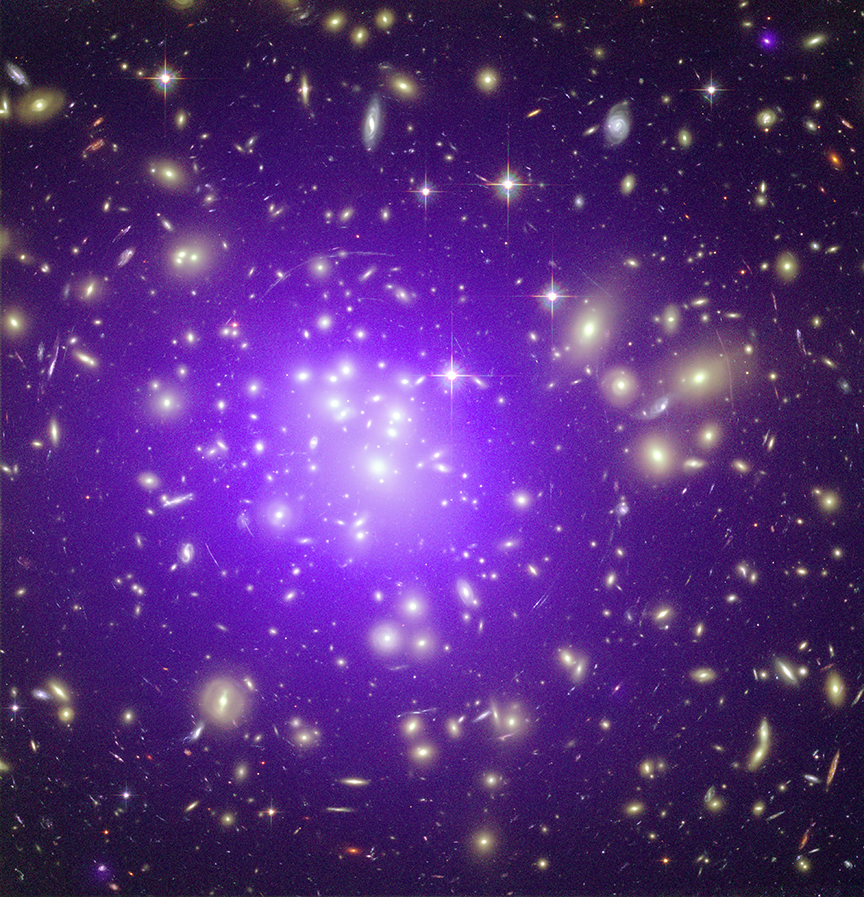
\includegraphics[width=0.5\textwidth]{images/Chapter2/a1689.jpg}
 \caption{Composite image of the galaxy cluster Abell 1689. Visible light is shown in yellow and X-ray in violet \citep{hubble-2010}}
 \label{fig:Abell1689}
\end{figure}

To investigate the X-ray spectrum of a galaxy cluster consider \eqref{emiss}:

\begin{equation}
\label{emiss}
    \epsilon^{ff}_{\nu} = \frac{32\pi Z^2 e^6 n_e n_i}{3m_ec^3}\sqrt{\frac{2\pi}{3k_B T m_e}}e^{-hp\nu/k_B T}g_{ff}(T,\nu)
\end{equation}

\begin{equation}
\label{emiss_g}
g_{ff} \approx \frac{3}{\sqrt{\pi}}\ln{\frac{9k_B T}{4h_P \nu}} \approx 1
\end{equation}

$\epsilon^{ff}_{\nu}$ is the emissivity of the bremsstrahlung where Z is the charge of the ions, $e$ the elemental charge, $n_e$ and $n_i$ the electron and ion density, $h_P \nu$ the photon energy, $k_BT$ the thermal energy, $m_e$ the electron mass, $c$ the speed of light and $g_{ff}$ the Gaunt factor which takes quantum mechanical effects into account. For classical problems $g_{ff}$ is set to $1$.

Using this equation, one finds a flat continuity region for $h_p \nu \ll k_B T$. This continuity region is cut off exponentially for higher energies ($h_p \nu > k_B T$). Photoabsoption cuts off the lowest energy part of the continuity region giving us the spectrum in \autoref{fig:x-ray_emission_curves}

\begin{figure}[h]
 \centering
 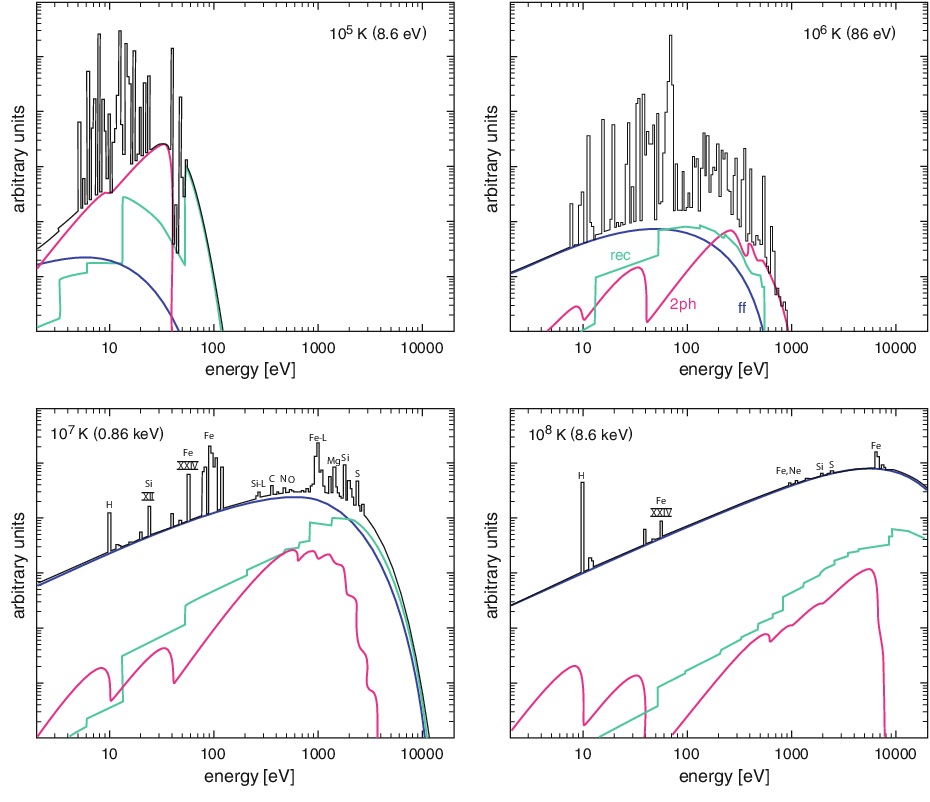
\includegraphics[width=1\textwidth]{images/Chapter2/9-Figure6-1.png}
 \caption{Free free radiation at different plasma temperatures including photo absorption (blue). Recombination radiaton (green) and two-photon radiation (red) are shown for comparison of the dominating source of radiation. Absorption and emission lines are shown in black.  \citep{Boehringer2010}}
 \label{fig:x-ray_emission_curves}
\end{figure}

In the case of galaxy clusters, we have temperatures $> 10^6K$ making the X-ray radiation the spectrum's dominant part. Emission lines become more disruptive at lower temperatures whilst at $T > 10^7K$ especially the emission from iron and silicon are most notable.

Using this relation between the X-ray spectrum and the plasma temperature, it is possible to estimate cluster temperatures. Moreover, it is possible to use this knowledge to work out scaling relations to estimate galaxy cluster masses (see \cref{mass_est}).

\subsection{Why are we Interested in Galaxy Masses and why do we use X-rays for this?}
\begin{figure}[h]
 \centering
 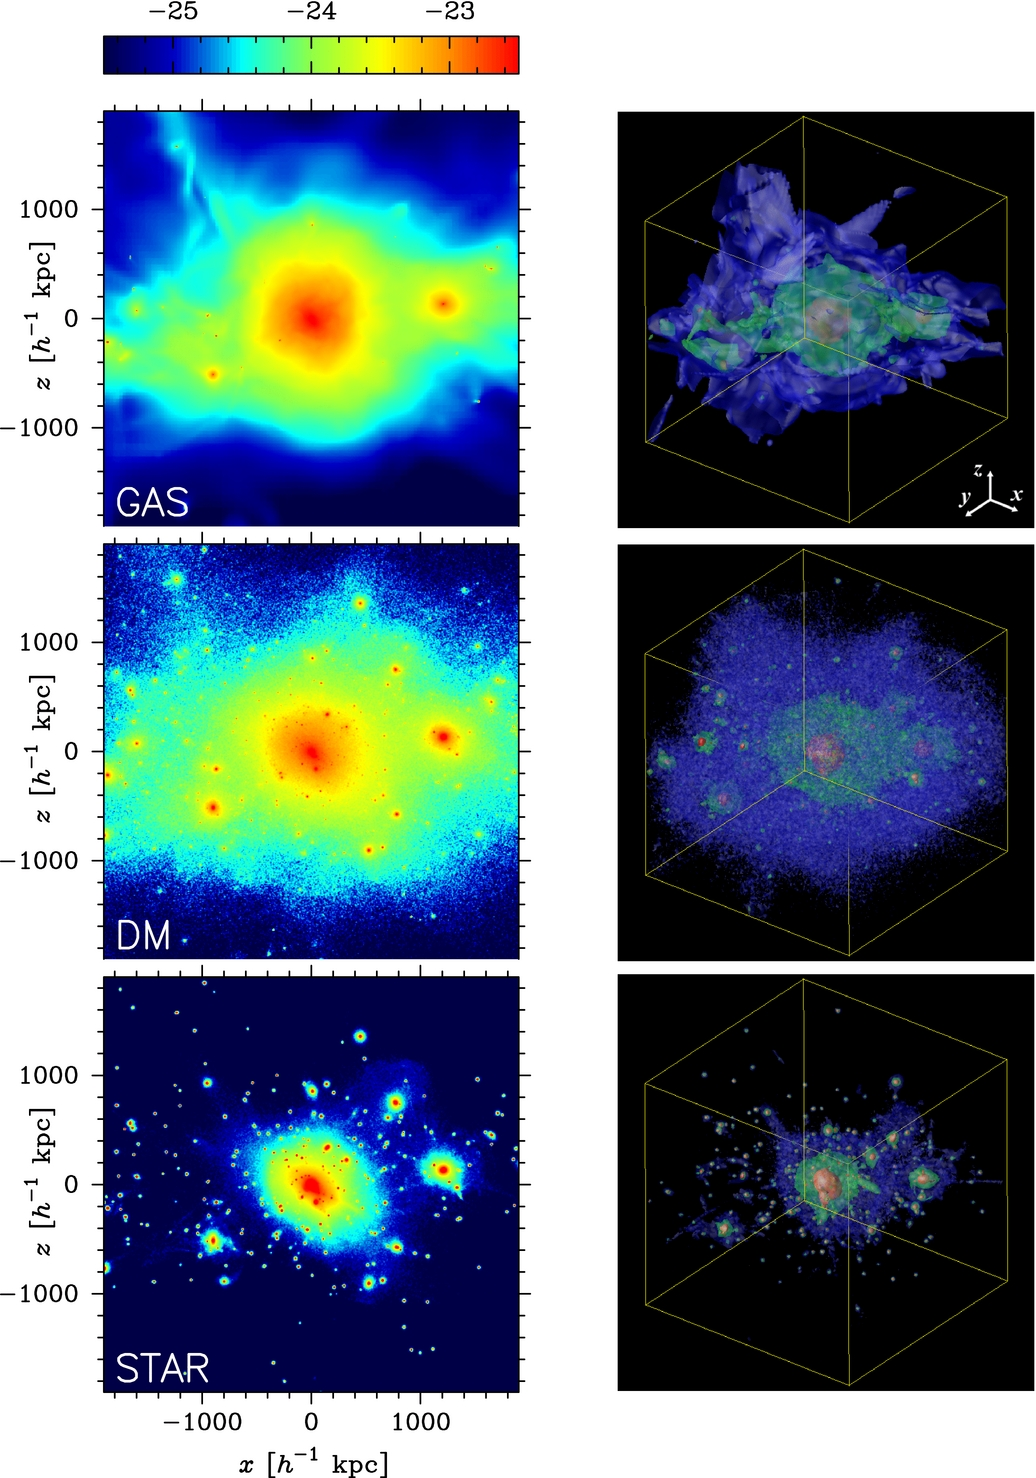
\includegraphics[width=0.6\textwidth]{images/Chapter2/apj464555f1_hr.jpg}
 \caption{Simulation of a galaxy cluster. The first row shows the gas density, the second shows the dark matter density and the last shows the star distribution. The right column shows a 3D rendering of the cluster while the left column shows a projection on the x-z plane.  \citep{Suto_2013}}
 \label{fig:cluster_sim_dm}
\end{figure}

Prior to discussing methods for estimating the masses of galaxy clusters, I'd like to point out the significance of understanding these masses in the first place.

In 1933 Fritz Zwicky was the first one who brought up, that the mass of visible matter of galaxy clusters would be way too small to explain the high movement speeds of the individual galaxies of more than $1000 \, km\cdot s^{-1}$. He estimates, that the cluster mass would have to be 400 times higher as approximated to explain this discrepancy. \citep{Zwicky_1933} To solve this issue, he proposed that the majority of the cluster mass is made out of dark matter causing the observed speeds. Although disputed at first, Zwicky's assumptions are now the basis for dark matter astronomy making galaxy clusters the most important laboratories in the cosmos. To understand the nature of dark matter, it is of key importance to know the cluster masses. Only with precise values, galaxy cluster dynamics such as merges can be accurately observed. More recent simulations of the cluster's dark matter halo show, that the gas distribution is very similar to the distribution of dark matter as seen in \autoref{fig:cluster_sim_dm}. As discussed in \cref{x-ray}, X-ray light is directly being emitted by the hot cluster gas. For this reason, X-ray satellites such as CHANDRA and eROSITA are the best observatories for understanding the distribution of dark matter in galaxy clusters.



\subsection{Estimating the Mass of a Galaxy Cluster}
After explaining how the spectrum of a galaxy cluster looks like in \cref{x-ray}, I will explain how to estimate a galaxy cluster's mass using this spectrum and other techniques.
\subsubsection{Traditional Mass Estimation using Observational Data}
\label{mass_est}
To estimate galaxy cluster masses using observational data, we first have to check whether the plasma that emits the X-ray spectrum is in a state of equilibrium. Otherwise we cannot use simplifications for the hydrostatic equilibrium of the ICM. In order to verify that, consider the ICM's speed of sound

\begin{equation}
\label{c_s}
    c_s \approx \sqrt{\frac{P}{\rho_g}} = \sqrt{\frac{nk_B T}{\rho_g}} = \sqrt{\frac{k_B T}{\mu m_p}} \sim 1000 \frac{km}{s}
\end{equation}
\begin{equation}
    \mu := \frac{<m>}{m_p}
\end{equation}

where P is the gas pressure, $\rho_g$ the density of the gas, n the number of gas particles, $m_p$ the proton mass and $\mu$ the mean molecular mass in respect to the mass of a proton.
The mean molecular mass for a fully ionized hydrogen plasma is $\mu = 0.5$ because there is roughly one proton and one electron for every proton mass. Considering that there are also heavier elements in the ICM, $\mu$ can be estimated to $\mu \sim 0.6$ \citep{Ettori_2019}. For a galaxy cluster with a temperature of $10^8 K$ we optain a speed of sound of $\sim 1000 \, km \cdot s^{-1}$. For a galaxy cluster with a radius of $10^7ly$ this gives a travel time of $\sim 10^9$ years. Taking into account that the cluster age can be estimated with the age of the cosmos \citep{Rakos_2006}, this gives enough time for the ICM to be in a state of equilibrium, especially for the central part where most of the X-ray emission comes from.
For an equilibrium between the gas pressure and the gravitational force we obtain

\begin{equation}
    \nabla P = - \rho_g \nabla \Phi,
\end{equation}

where $\Phi$ is the gravitational potential. Assuming a spherical symmetry the potential is given by

\begin{equation}
    \Phi(r) = - \frac{GM}{r},
\end{equation}

where $G$ is the gravitational constant, $M$ a mass and $r$ the distance to the mass observed. This leads to

\begin{equation}
\label{dif_1}
    \frac{1}{\rho_g}\frac{dP}{dr} = - \frac{GM(r)}{r^2},
\end{equation}

where $M(r)$ is the mass within the radius $r$ including the gas mass, stellar mass and the dark matter mass. As used in \eqref{c_s} the gas pressure is given by $P = \rho_g k_B T/(\mu m_p)$. Solving the differential equation \eqref{dif_1} for $M(r)$ we yield 

\begin{equation}
    M(r) = - \frac{k_B T r^2}{G\mu m_p}\left( \frac{d\ln \rho_g}{dr} + \frac{d\ln T}{dr} \right)
\end{equation}

for the mass of a galaxy cluster. The cluster temperature can be evaluated with the X-ray spectrum as discussed in \cref{x-ray} leaving the gas density as the only remaining unknown. A powerful tool to evaluate the gas densities is the $\beta$-model \citep{Cavaliere_1976}. 
It assumes that the velocity distribution of the gas is the same as the velocity distribution of the visible and dark matter. This gives a relation between the gas density and the cluster density

\begin{equation}
    \rho_g (r) \propto \left[ \rho (r) \right]^{\beta}
\end{equation}

with

\begin{equation}
    \beta = \frac{\mu m_p \sigma_v^2}{k_BT_g},
\end{equation}

where $\sigma_v$ is the velocity distribution of the galaxy cluster. Using this relation, the X-ray spectrum can be modelled as

\begin{equation}
    I(R) \propto \left[ 1 + \frac{R}{r_c}^2 \right]^{-3\beta + 1/2},
\end{equation}

where $r_c$ is the central radius.
This tool-set provides everything needed to evaluate the masses of galaxy clusters. Using the virial theorem, scaling relations between the cluster temperature, mass and radius can be obtained giving us

\begin{equation}
    T \propto \frac{M_{vir}}{r_{vir}} \propto r^2_{vir} \propto M^{2/3}_{vir},
\end{equation}
where $M_{vir}$ and $r_{vir}$ is the mass and radius for which the virial theorem can be used. Typical values of $r_{vir}$ are radii, for which the cluster density is 200 times higher as the critical density of the universe. Sometimes a value of 500 times the critical density is being used, because it is easier to evaluate the mass $M_{500}$ than the mass $M_{200}$.
\\

Rating the accuracy of this approach, it must be said that both the assumptions of a homogeneous gas and temperature distribution seem to be only partially correct. The gas temperature profile can be dominated by the emission from more dense regions, resulting in a higher measured temperature. Moreover, it has been shown that the temperature has a gradient, dropping towards the cluster's edge \citep{McCourt_2013}.
Because of this uncertainties, different ways of estimating cluster masses are of great importance.

It is also worth noting that the masses of galaxy clusters can be estimated in a different way. Because of the enormous mass of galaxy clusters, they bend the space-time in such a way, that light travelling through the cluster is bend. Considering how exactly the light is bend, it is possible to estimate the mass of a galaxy clusters. This technique is used to calibrate observational data of sky surveys such as eROSITA's eFEDS \citep{Chiu_2022}.
\subsubsection{A new Approach using Convolutional Neural Networks}
\label{new_approach}
Within the last few years, the usage of convolutional neural networks (CNNs) has exploded. While in 2018 around 50 papers where published who used CNNs for astrophysical problems, the number of publications has tripled to around 150 in 2022\footnote{Numbers from https://arxiv.org/}. To this date, there are only a few approaches to infer galaxy masses with CNNs. Usually, a simulation set is needed in order to train the neural network. Because by training with data from let's say the mass estimation mentioned in \cref{mass_est}, the neural network would never be able to get a more accurate result than the data it was being trained with. That's why simulations are needed where the exact cluster mass is known. Luckily, these are being generated anyway for many missions such as Chandra and eROSITA to be able to prepare data analysis methods before the start of the actual mission. For instance \citet{Ntampaka_2018} used mock data for the Chandra X-ray satellite to train a CNN. Especially important for my thesis is the development of a neural network for eROSITA's \textit{Final Equatorial-Depth Survey} (eFEDS). \citet{Krippendorf_2023} used galaxy cluster data specifically simulated for eFEDS' observational data to train a CNN for mass estimation. The simulation data includes ten frequency bands and redshift data (see \cref{data_catalogue}). This approach used a comparably simple architecture, being the baseline for my development of a deep neural network using the same data set (see \cref{training}). Being able to infer galaxy cluster masses in many different ways is a great way to improve the accuracy of missions' data. AI and especially CNNs play an important role in receiving higher accuracies. How they work and why they are used is being discussed in \cref{CNN Structure}.

\subsection{The Structure of Convolutional Neural Networks}
\label{CNN Structure}
Amongst different neural network architectures, CNNs proved to be very successful in image recognition. The \textit{ImageNet Large Scale Visual Recognition Challenge} (ILSVRC) is a competition for algorithms to classify images from the ImageNet catalogue and was held between 2010 and 2017. Since 2012, every winning neural network was a convolutional neural network, jumping from a 28\% top-5 error in 2010 to a 2.3\% error in 2017. Two main improvements are responsible for this rapid increase in accuracy:\\

\begin{enumerate}
    \item Usage of GPUs for training
    \item Development of deeper convolutional neural networks
\end{enumerate}

Because of the similarity in task between ImageNet classification and galaxy cluster mass estimation (see \autoref{fig:imagenet_clusters}), I expect the ILSVRC successor's architectures (VGG\footnote{\citet{Simonyan_2015}} and ResNet\footnote{\citet{He_2016}}) to do well with our task. Therefore I want to examine their performances with our problem and compare it to a more recently developed model. 

\subsubsection{A Basic Convolutional Neural Network}
\label{basic_cnn}
Convolutional neural networks can have many different architectures where at least one step of the algorithm features a convolution. 
\subsubsection*{Convolutions}

The mathematical form of a convolution of two functions $f$ and $g$ is given by

\begin{equation}
    (f \ast g)(t) = \int_{-\infty}^{\infty}f(\tau)g(t-\tau)d\tau, 
\end{equation}

which evaluates how the shape of $f$ is modified by $g$. Because image data is only an array of photon counts we can use the discrete convolution

\begin{equation}
    (f \ast g)(t) = \sum_{\tau=-\infty}^{\infty}f(\tau)g(t-\tau).
\end{equation}

In our case, $f$ and $g$ will be tensors. Usually $f$ is called the \textit{input}, $g$ the \textit{kernel} or \textit{filter} and the convolution $(f \ast g)(t)$ the \textit{feature map}. Since our galaxy cluster data is multi-dimensional (see \cref{data_catalogue}), we also have to use a multi-dimensional convolution


\begin{equation}
\begin{split}
    &(f \ast \overset{M}{\cdots} \ast g)(t_1,t_2,\dotsc,t_M) = \\ 
    = \sum_{\tau_1 = - \infty}^{\infty} \sum_{\tau_2 = - \infty}^{\infty} \cdots \sum_{\tau_M = - \infty}^{\infty} &g(\tau_1,\tau_2,\dotsc,\tau_M) f(t_1 - \tau_1, t_2 - \tau_2, \dotsc, t_M-\tau_M).
\end{split}
\end{equation}

For two-dimensional tensors the convolution process can be seen in \autoref{fig:conv_ex}.

\begin{figure}[ht]
 \centering
 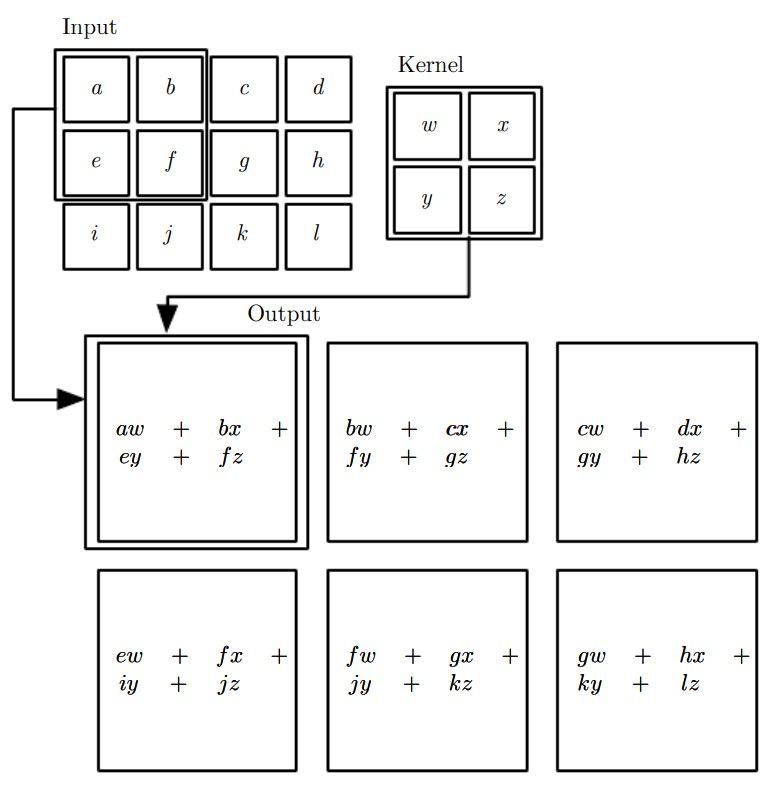
\includegraphics[width=0.66\textwidth]{images/Chapter2/tensor_conv.jpg}
 \caption{Example of a 2D-convolution for an image input with a dimension of 4x3 pixels and a 2x2 kernel resulting in a 3x2 feature map. \citep{Goodfellow-et-al-2016}} 
 \label{fig:conv_ex}
\end{figure}

Training a CNN, we allow the algorithm to evaluate different kernels to help classifying the image. It has been shown that edge detection is one of the most important aspects of image classification. For example the kernel 

\begin{gather}
    g = \begin{bmatrix}
0 & -1 & 0\\
-1 & 4 & -1 \\
0 & -1 & 0
\end{bmatrix}
\end{gather}

is able to highlight edges from input images. To get an idea of how this is executed consider \autoref{fig:seagull}.


\begin{figure}[ht]
 \centering
 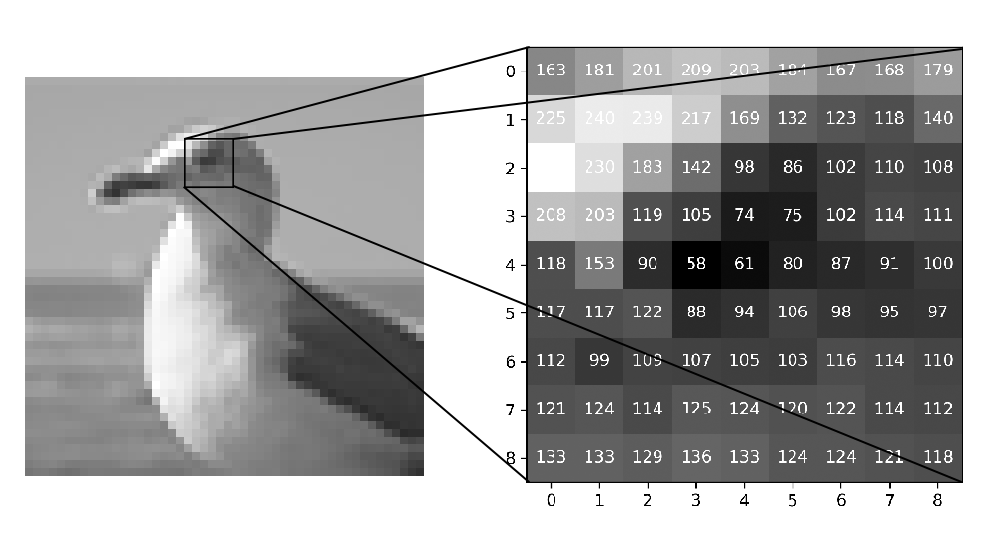
\includegraphics[width=0.66\textwidth]{images/Chapter2/eye_array.png}
 \caption{Image of a seagull in black and white with a size of 50x50 pixels. Every pixel has a value from 1 to 255 indicating its brightness as seen on the right with an extract of 9x9 pixels. By converting this image into a tensor, it is possible to do a two dimensional convolution.} 
 \label{fig:seagull}
\end{figure}
\newpage

Taking only the seagull's eye as input, our tensor has the following shape:

\begin{gather}
    f = \begin{bmatrix}
163 & \cdots & 179\\
\cdots & \cdots & \cdots \\
133 & \cdots & 118
\end{bmatrix}
\end{gather}

Applying the convolution on the whole image we indeed get an outline of the seagull's shape.

\begin{figure}[ht]
 \centering
 
\includegraphics[width=0.4\textwidth]{images/Chapter2/2DConvolved.jpg}
 \caption{Image from \autoref{fig:seagull} after the convolution with the edge outlining kernel $g$.} 
 \label{fig:seagull_conv2d}
\end{figure}

This method indicates why CNNs are so powerful when it comes to image classification. Being able to train and develop filters that can manipulate the input in such a way that it is easier to see patterns, is crucial. \\
Most CNNs are not only build up with convolutions alone. In most cases the combination of one or more convolutions with different mathematical operations helps to increase accuracy. One of these operations is \textit{pooling}.

\subsubsection*{Pooling}
Pooling is another algorithm that helps to simplify the input signal. There are two main pooling operations in machine learning:

\begin{enumerate}
    \item average pooling
    \item max pooling
\end{enumerate}

Although they work in a slightly different manner, they serve the same purpose: helping with translations. If a neural network is supposed to find a certain feature within an image, in most cases it is not necessary to know where the feature is located within the image. Reducing the input to a smaller tensor also helps with training speeds. Average pooling takes the sum over a specific area of the input signal. For example a pooling with a stride of two (see \autoref{fig:pooling}) takes the input of four neighbouring values and reduces them to their average. Max pooling works in a very similar fashion but instead of reducing the neighbouring values to their average, it only keeps the maximum value.

\begin{gather*}
\begin{bmatrix}
\color{green} 50 & \color{blue} 100\\
\color{red} 166 & \color{orange} 24 
\end{bmatrix}
\overset{\text{avg pooling}}{\longleftarrow}
\begin{bmatrix}
\color{green} 163 & \color{green} 17 & \color{blue} 179 & \color{blue} 123\\
\color{green} 0 & \color{green} 21 & \color{blue} 89 & \color{blue} 10 \\
\color{red} 173 & \color{red} 196 & \color{orange} 9 & \color{orange} 15 \\
\color{red} 175 & \color{red} 118 & \color{orange} 62 & \color{orange} 12
\end{bmatrix}
\overset{\text{max pooling}}{\longrightarrow}
\begin{bmatrix}
\color{green} 163 & \color{blue} 179\\
\color{red} 196 & \color{orange} 62 
\end{bmatrix}
\end{gather*}
\captionof{figure}{An input tensor is reduced from 4x4 to 2x2 pixels using average pooling (\textit{left}) and max pooling (\textit{right}) with a stride of two. The colours represent the areas over which the averaging or maximizing takes place.}
\label{fig:pooling}
$\\$
Using these processes with our convoluted image from \autoref{fig:seagull_conv2d}, we can see the effect it has on the input signal.


\begin{figure}[h]
\begin{subfigure}{.5\textwidth}
  \centering
  
\includegraphics[width=.6\linewidth]{images/Chapter2/avg_pooling.png}
  \caption{Average pooling}
  \label{fig:sfig1}
\end{subfigure}%
\begin{subfigure}{.5\textwidth}
  \centering
  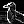
\includegraphics[width=.6\linewidth]{images/Chapter2/max_pooling.png}
  \caption{Max pooling}
  \label{fig:sfig2}
\end{subfigure}
\caption{The different output from pooling of the 48x48 pixel feature map (\autoref{fig:seagull_conv2d}). Both images show less details but preserve the seagull's shape} 
\label{fig:fig}
\end{figure}

While the main features are preserved, the pooling stage reduces complexity and makes training the network more efficient. If we want to do multiple convolutions, we need a way to keep its focus on basic features. As you can see in \autoref{fig:fig}, it is impossible to locate the seagull's eye. But if we just want to know whether we see a seagull or a hummingbird for instance, the exact position of the bird's eye is not that important. This helps to get a higher accuracy and efficiency.
\subsubsection*{Activation Function}
One last missing piece in our CNN block is the activation function. If a CNN block would just consist of convolutions and pooling, it would not be able to find complex features within an input. This is due to the fact that convolutions produce linear activations. This means that the more complex our network gets, we still only have linear connections between the network's layers. While this would work for simple linear regression problems, it is not possible to perform image classification with linearities. To avoid this problem, a non linear function is applied to every block's output. There are a lot of different non linear activation functions with different areas of application. The most simple activation function would be the step function (\autoref{fig:step_f})

\begin{equation}
    f(x) = \begin{cases} \mbox{0} & \mbox{for } x \leq 0 \\ \mbox{1} & \mbox{for } x > 0 \end{cases}.
\end{equation}
Every positive value of the feature map receives the value $1$ while every negative value is changed to $0$. Although this would technically deal with the linearities, it removes most of the details from the input and it would only be useful if we want a binary output. \\

Another option is the hyperbolic tangent function (\autoref{fig:hyptg})

\begin{equation}
    f(x) = \tanh{x} = \frac{e^x - e^{-x}}{e^x + e^{-x}}.
\end{equation}
It can produce values from $-1$ to $1$ and keeps more details than the step function. Activation functions with an output of $-1$ to $1$ or $0$ to $1$ are useful for applications where a possibility should be evaluated.

For more complexity, the rectified linear unit function (ReLU) can be used (\autoref{fig:ReLU})

\begin{equation}
    f(x) = \text{max}(0,x) = \begin{cases}
        \mbox{x} & \mbox{for } x > 0 \\ \mbox{0} & \text{otherwise}
    \end{cases}.
\end{equation}

It leaves positive values unchanged while setting every negative value to zero. It is commonly used in many machine learning approaches because it is very effective in preserving complex details by keeping computing efficiency. Its only downside is the so-called \textit{dying ReLU} problem. If too many activations are set to zero, the neural network is not able to learn anything new. One way to solve this issue is by not setting the negative values to zero, but applying a scaling factor $a$ (usually $0.1$) to them:

\begin{equation}
    f(x) = \begin{cases}
        x & \mbox{for } x > 0 \\ ax & \text{otherwise}
    \end{cases}, \: a = 0.1 \,.
\end{equation}

This is called the Leaky ReLU function (\autoref{fig:L_ReLU}). Despite solving the dying ReLU problem, Leaky ReLU is not always the first choice for machine learning because it also increases computation effort. So it makes sense to first use ReLU and in case of bad predictions switch to other activation functions in optimization.


\begin{figure}[h]
\begin{subfigure}{.5\textwidth}
  \centering
  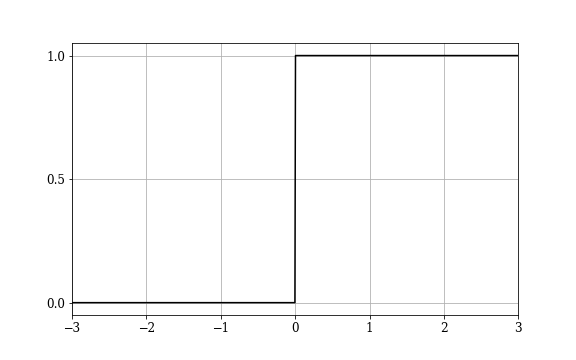
\includegraphics[width=\linewidth]{images/Chapter2/step (1).png}
  \caption{Step function}
  \label{fig:step_f}
\end{subfigure}%
\begin{subfigure}{.5\textwidth}
  \centering
  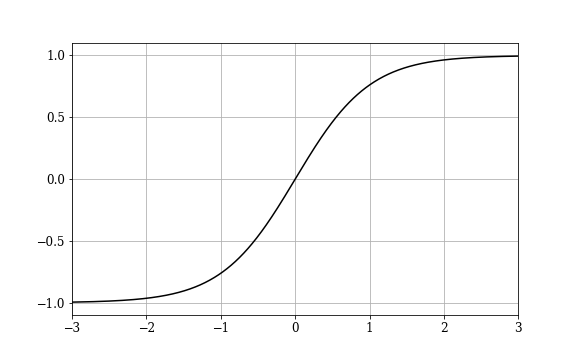
\includegraphics[width=\linewidth]{images/Chapter2/tanh (1).png}
  \caption{Hyperbolic tangent}
  \label{fig:hyptg}
\end{subfigure}
\begin{subfigure}{.5\textwidth}
  \centering
  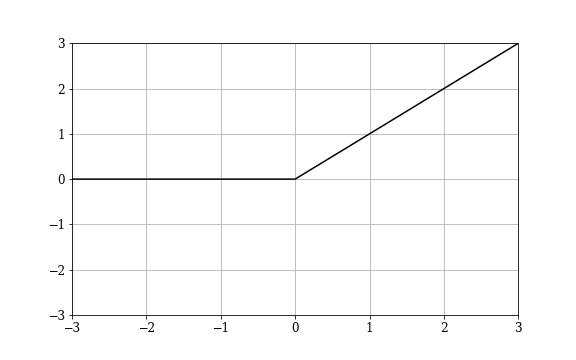
\includegraphics[width=\linewidth]{images/Chapter2/ReLU (1).png}
  \caption{ReLU}
  \label{fig:ReLU}
\end{subfigure}
\begin{subfigure}{.5\textwidth}
  \centering
  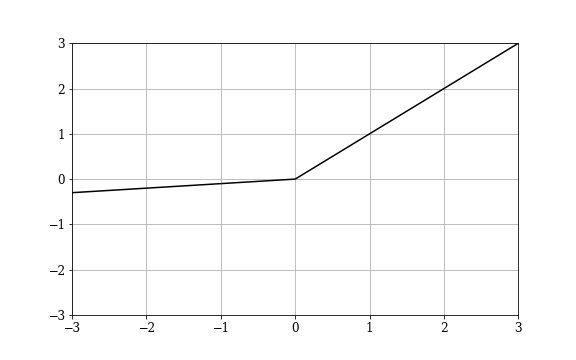
\includegraphics[width=\linewidth]{images/Chapter2/L_ReLU.png}
  \caption{Leaky ReLU ($a=0.1$)}
  \label{fig:L_ReLU}
\end{subfigure}
\caption{Plots of the four different activation functions mentioned} 
\label{fig:activ_functions}
\end{figure}


\subsubsection*{A Basic CNN Block}
Using these three different methods, it is possible to build a simple CNN block (\autoref{fig:CNN_Blocks}). The input tensor is fed into the convolution. Afterwards the feature map is processed via the activation function before applying a pooling. \\
This block can be altered or refined to suit a certain application but you will find this structure in basically every CNN. \citet{Krippendorf_2023} used a slightly altered basic CNN block (\autoref{fig:CNN_Blocks}) consisting of two two-dimensional convolutional layers with ReLU as activation function, average pooling in the first and max pooling in the second layer. 

\newpage

\begin{figure}[h]
\centering
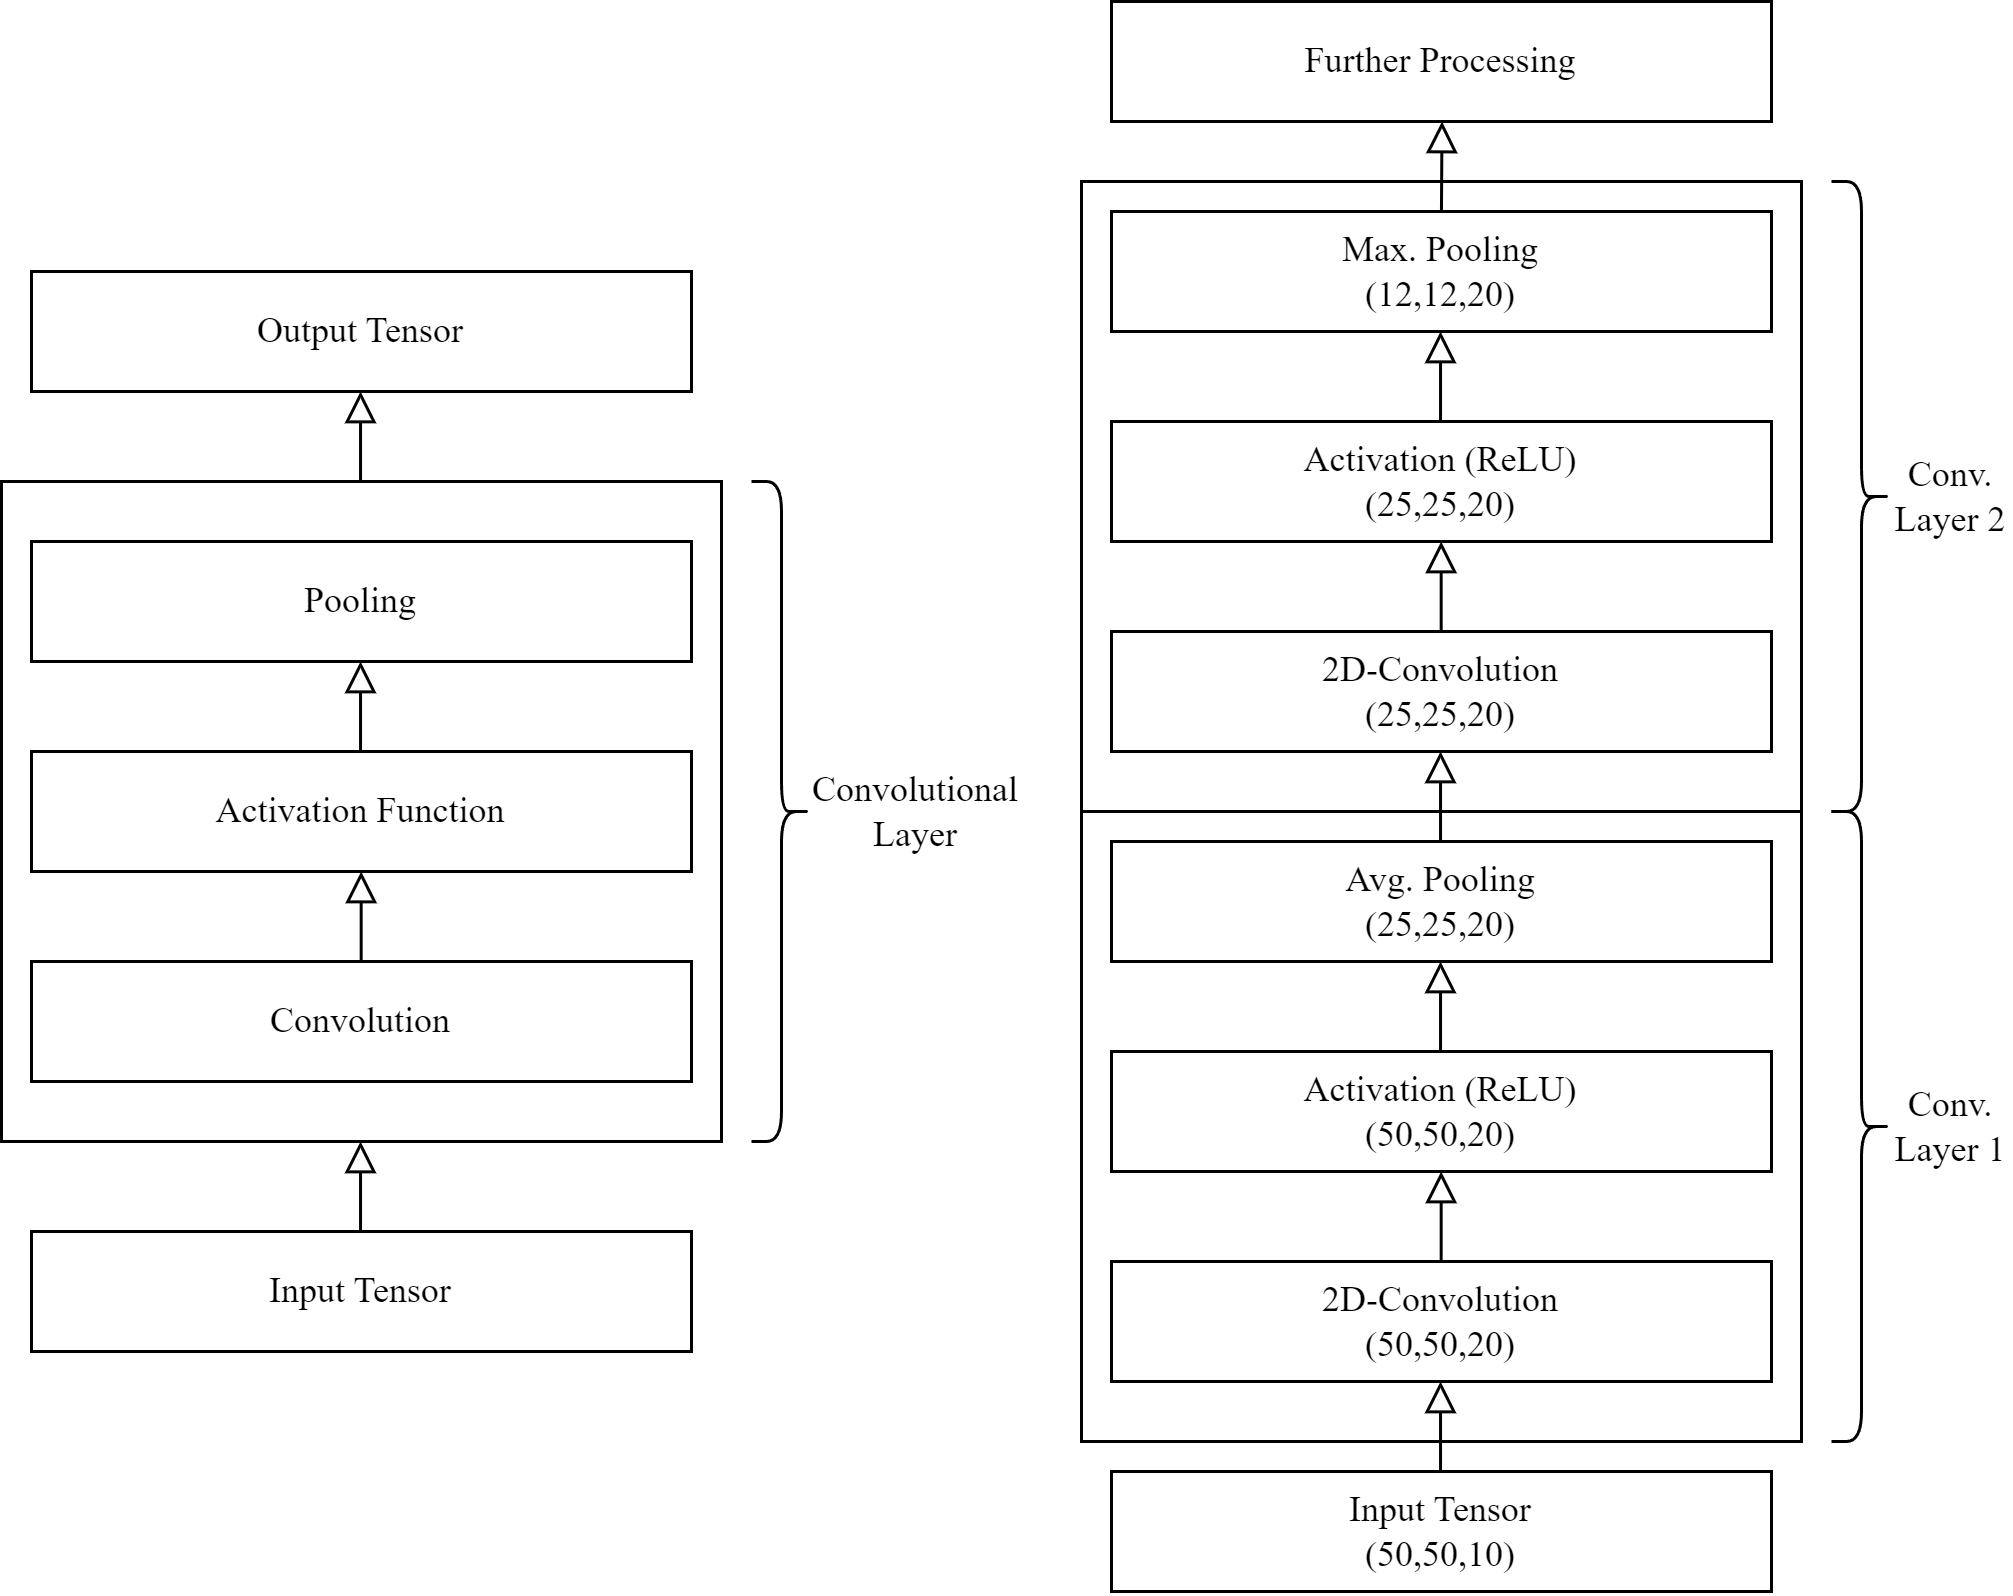
\includegraphics[width=\textwidth]{images/Chapter2/basic_cnn.png}
\caption{Diagrams of a basic CNN structure (\textit{left}) and its application for cluster mass estimation (\textit{right}) (as used in \citealp{Krippendorf_2023}). The convolution, activation and pooling block is referred to as \textit{convolutional layer}. In the application, two convolutional layers are used. The tensor shape is shown below each block.} 
\label{fig:CNN_Blocks}
\end{figure}


In this case, the output tensor of the convolutional layering has a shape of $(12,12,20)$, meaning an array of 12x12 pixels with 20 values for each pixel. However, we only want a single output value since we're interested in the mass of the evaluated galaxy cluster. To achieve this, the output tensor needs to be flattened. This operation puts every pixel and its 20 values into a single vector of the shape $(12\cdot 12 \cdot 20,0,0) = (2880,0,0)$. \\

At this point it is possible to put additional information into the neural network. Consider the \textit{inverse-square law}

\begin{equation}
    I \propto \frac{1}{r^2},
\end{equation}
where $I$ is the intensity of the received light and $r$ is the distance to the light source. This means that without knowing the distance to a light emitting object, it is not possible to estimate the total amount of radiated light. This however is crucial in comparing different galaxy clusters, because a galaxy cluster at a distance of $z=0.6$ can have the same measured intensity as a much bigger galaxy cluster at $z=1.2$.
Providing the neural network with this additional information is as easy as adding it to the vector generated by the flattening, resulting in a shape of $(2881,0,0)$. The next layer after processing the convolutional layer's output is the dense block. This block performs the actual classification of our input. 

\begin{figure}[h]
\centering
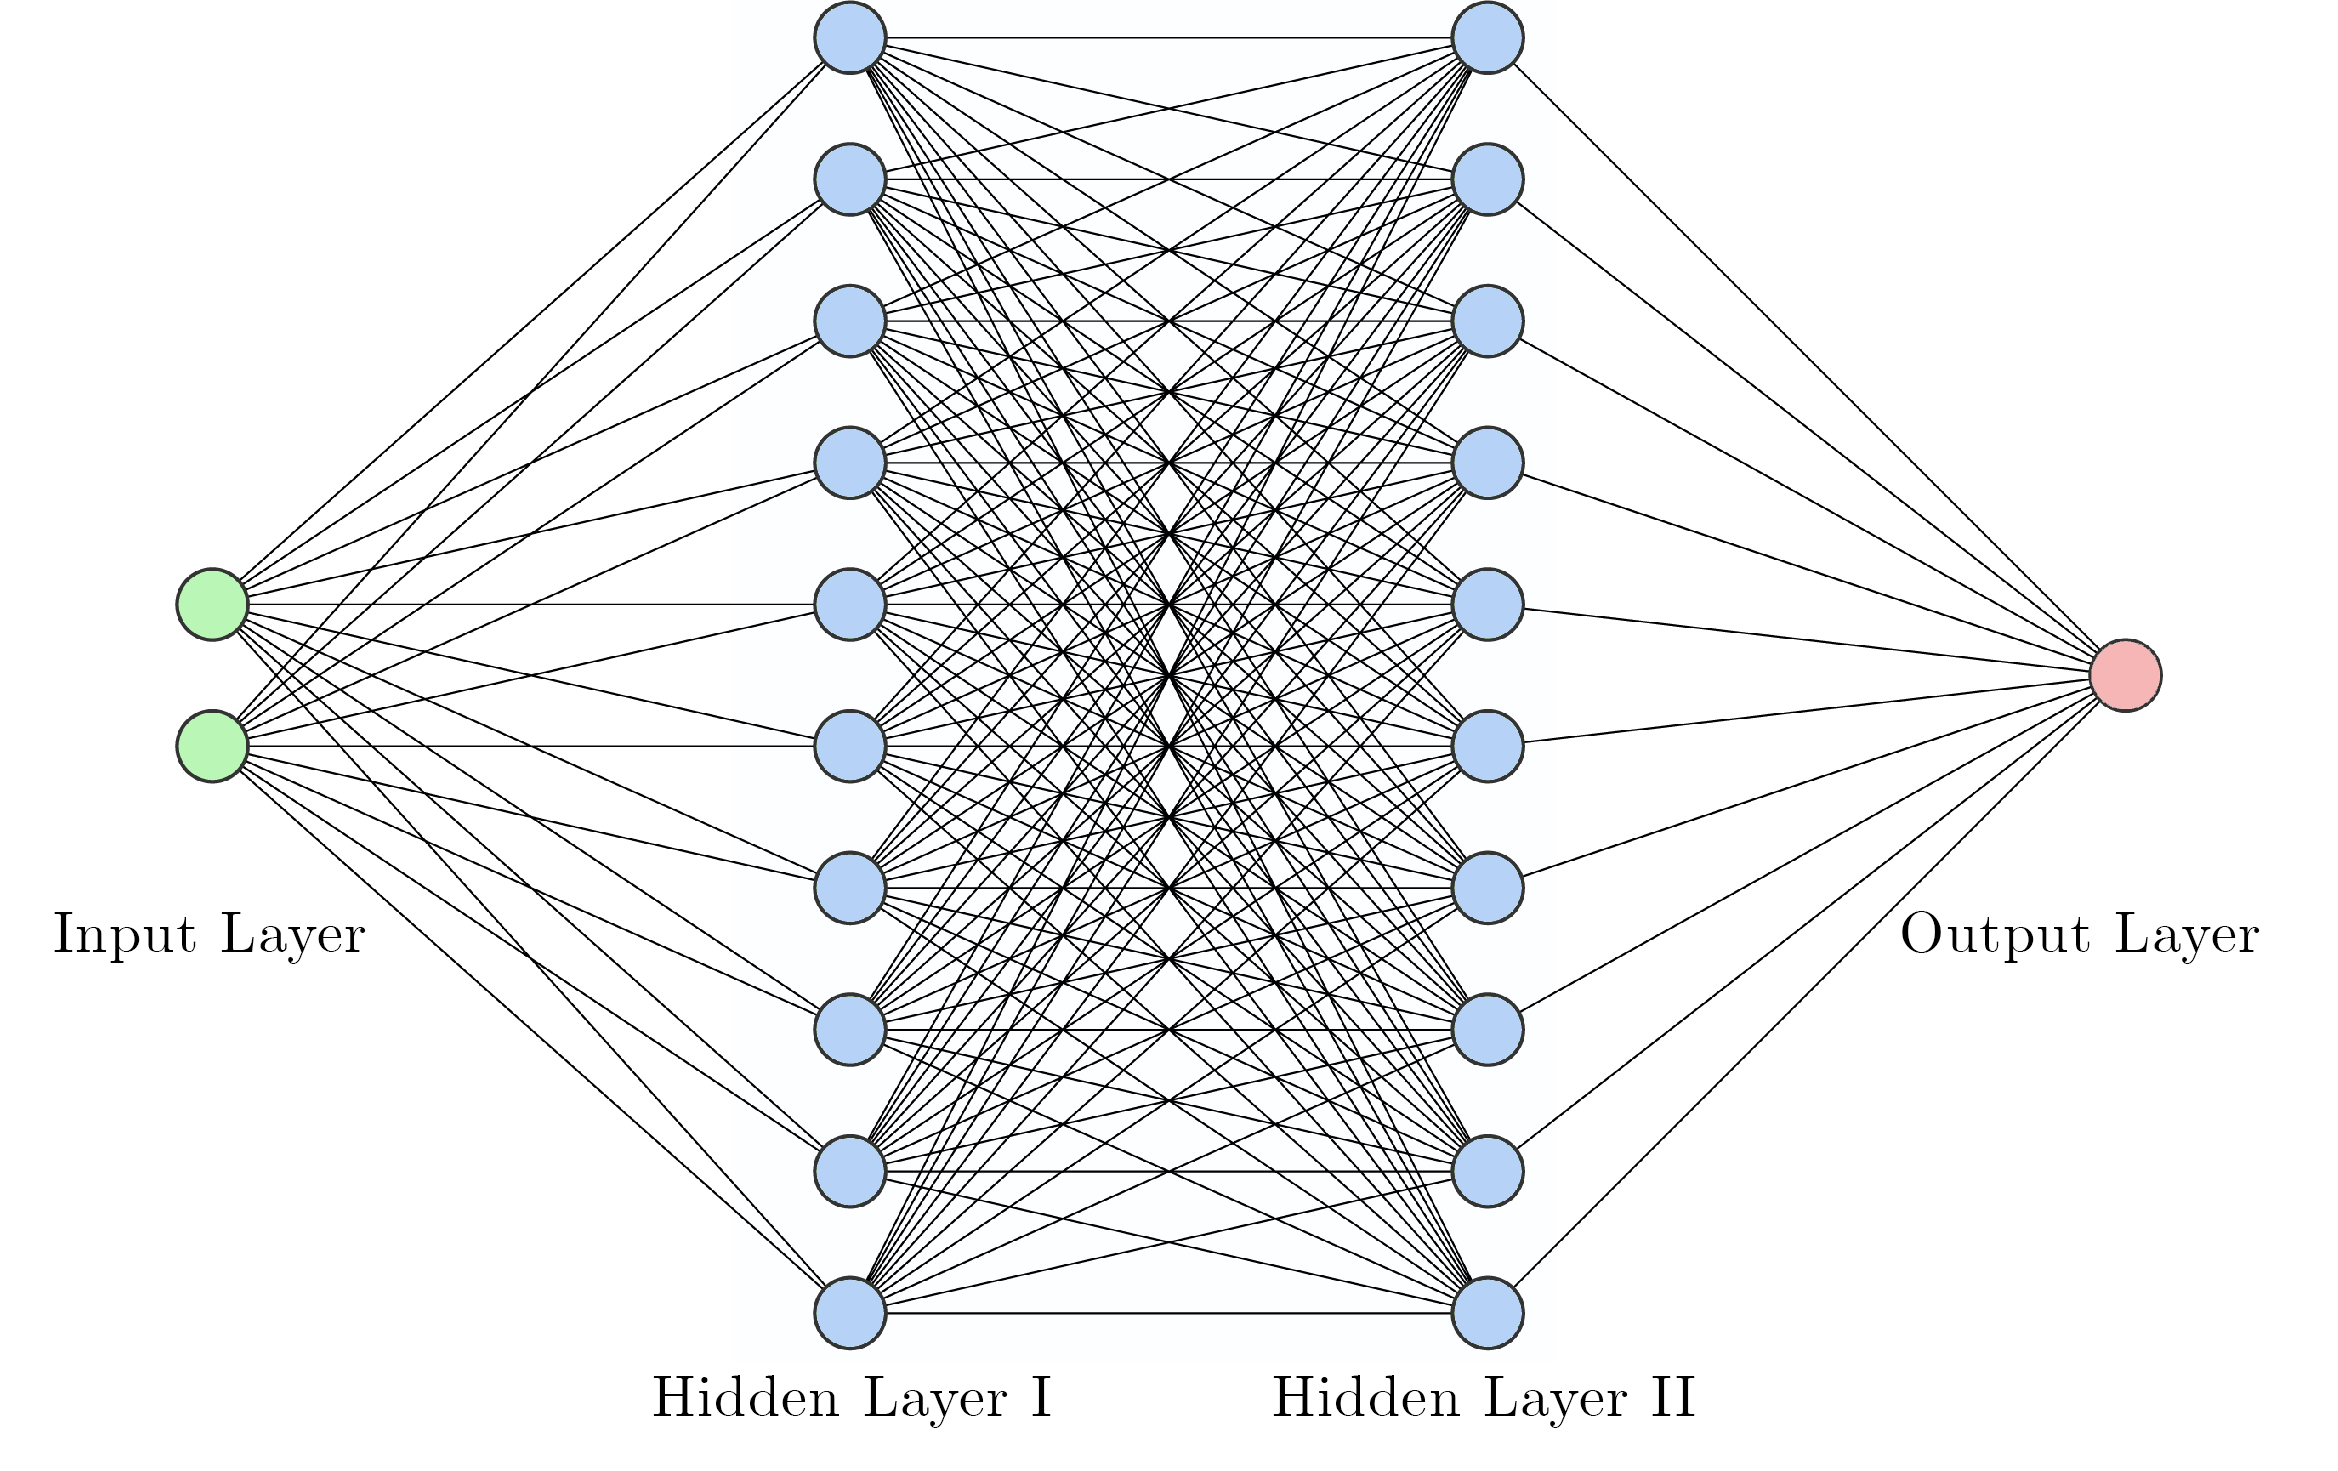
\includegraphics[width=0.9\textwidth]{images/Chapter2/nn.png}
\caption{A dense layer consisting of an input (\textit{green}), two hidden (\textit{blue}) and an output layer (\textit{red}). This can be thought of as the \textit{brain} of every neural network. } 
\label{fig:dense}
\end{figure}

A dense layer, often referred to as \textit{artificial neural network} (ANN) is based on the neuron structure of human and animal brains. It consists of units called \textit{neurons} that are connected to each other to be able to pass on signals. Mathematically, ANNs can be described as the sum of all connections leading to a neuron. For example a neuron $n_i$ receives an input value $x_i$ from a connection to a prior neuron. This specific connection is provided with a \textit{weight} $w_i$ which decides how important the input from this neuron is. Next, the sum over all connections to the neuron and their weights determines the value of this neuron $z$
\begin{equation}
\label{ann}
    z  = \sum \left( (w_1 \cdot x_1) + (w_2 \cdot x_2) + \cdots + (w_n \cdot x_n) \right) = \sum^n_{i=1} w_i \cdot x_i.
\end{equation}
The weights are not the only manipulable parameters. There's also an offset $b$ to the value calculated in \eqref{ann} called \textit{bias}.

\begin{equation}
\label{bias}
    Z  = z + b = \sum^n_{i=1} w_i \cdot x_i + b
\end{equation}
With bias, the algorithm can shift the weighted output in either direction for further evaluation of the importance of specific neurons. Here, another activation function $\Tilde{f}$ is needed in order to archive a certain output. This gives us the final formula for a neuron output with $n$ connections

\begin{equation}
    f(x_i,w_i,b,\Tilde{f}) =  \Tilde{f}(Z) = \Tilde{f} \left( \sum^n_{i=1} w_i \cdot x_i + b \right).
\end{equation}

The activation function is normally provided and tied to the classification task, leaving two trainable parameters, weight and bias.
To know in which direction a machine learning algorithm should alter the weights and biases, it must be provided with a function that needs to be optimised. This is called the \textit{cost} or \textit{loss function}. It provides the neural network with a way of knowing if it gets closer to the real values or not. A commonly used cost function is the \textit{mean squared error} (MSE)

\begin{equation}
\label{MSE}
    L \equiv \text{MSE} = \frac{1}{n}\sum^n_{i=1} \left( X_i - \Tilde{X_i} \right)^2,
\end{equation}

where $n$ is the number of values considered, $X_i$ is the actual given value and $\Tilde{X_i}$ the model's prediction. This function gives the average of the squared errors for a dataset and is used in a variety of machine learning problems. In order to optimise this function, the algorithm performs a \textit{gradient decent}. This means that after changing the weights and the biases, it takes the gradient of the loss function with respect to both parameters

\begin{equation}
    \nabla(L(\Tilde{f},w_i,b)) = \frac{\partial L}{\partial w_i}\hat{w_i}, \frac{\partial L}{\partial b}\hat{b},
\end{equation}
where $\hat{w_i}$ and $\hat{b}$ are unit vectors in the weight and bias space.

The updated parameters are calculated using
\begin{align}
    w_i^{\text{new}} &= w_i - \alpha \cdot \frac{\partial L}{\partial w_i} \; \; \text{and} \\
    b^{\text{new}} &= b - \alpha \cdot \frac{\partial L}{\partial b},
\end{align}

where $\alpha$ is the learning rate. It tells the algorithm how far it is allowed to go towards the gradient. Especially with overfitting problems, the learning rate must be chosen carefully. If an algorithm is learning too quickly, it can find a minimum in the loss function that might be a good fit for the input data but does not work with data is has not seen during training. We will address this issue in \cref{train_params}.\\

Finally we have a complete and trainable neural network (see \autoref{fig:final_network}) with multiple convolutional layers. 

\begin{figure}[H]
\centering
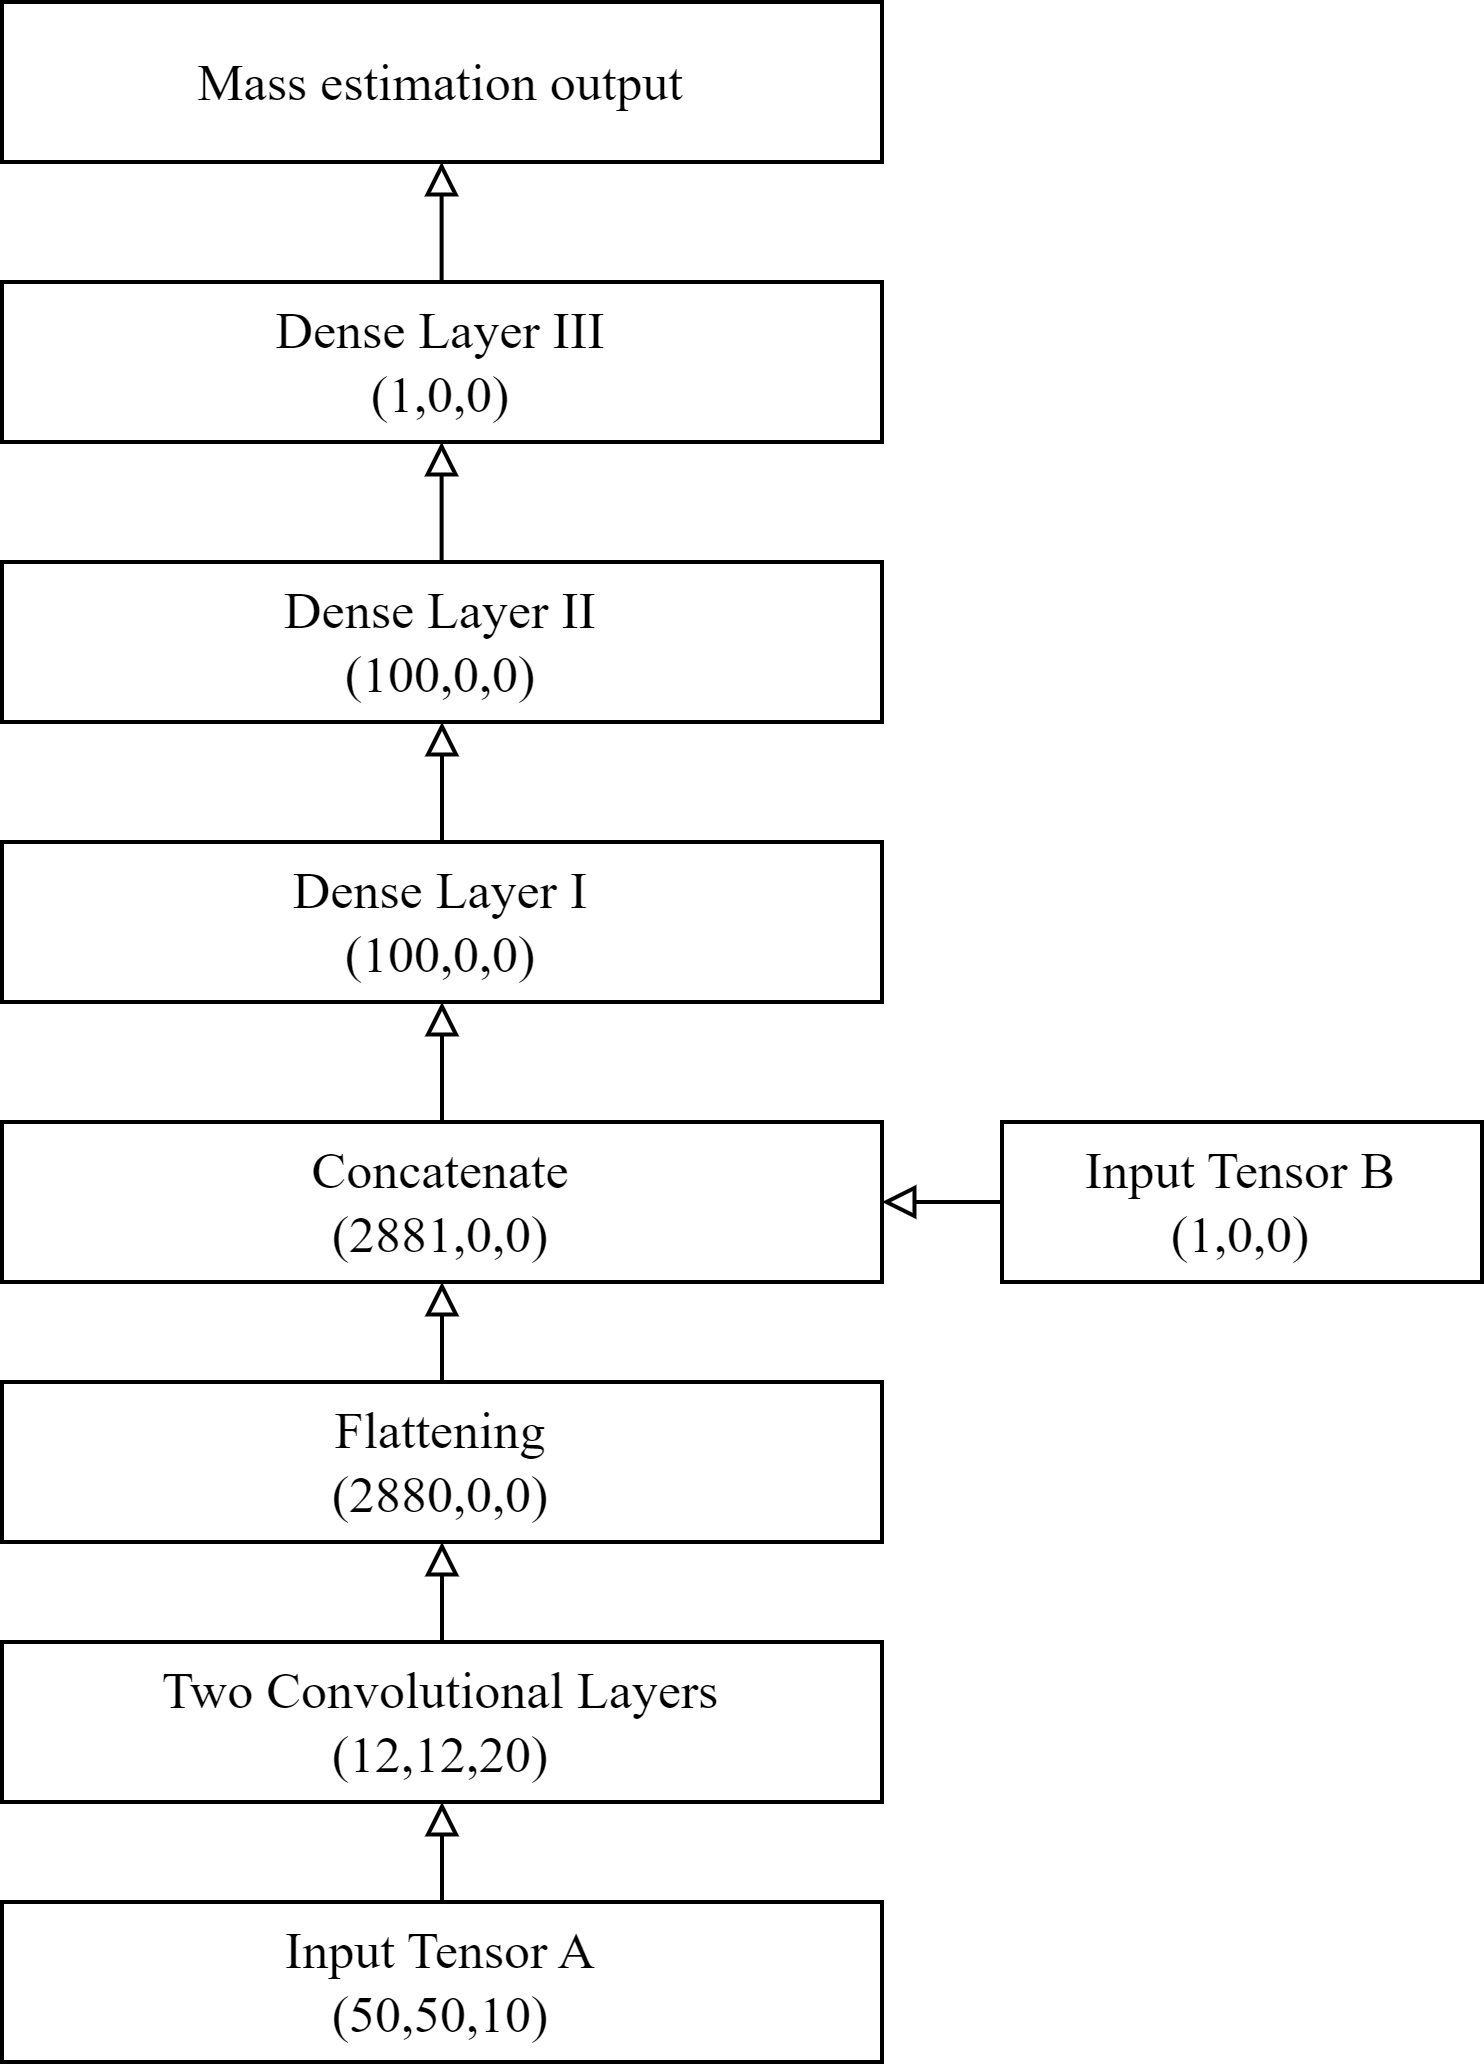
\includegraphics[width=0.4\textwidth]{images/Chapter2/basic.png}
\caption{The final processing of our convoluted input from \autoref{fig:CNN_Blocks}. The output tensor shape is shown below the block labeling. Input A is the input of the X-ray images and input B is the input of the redshift data.} 
\label{fig:final_network}
\end{figure}











\subsubsection{Deep CNNs}
As already mentioned, deep learning has really taken image classification to another level in the recent years. One could assume that it is as easy as using many convolutional layers in repeat to achieve this. However, training a neural network with a high depth was neither effective, nor more accurate. The deeper the input signal is forwarded into the network, the higher the chance for actually losing the signal is, leaving only noise instead of a signal to the dense layers. AlexNet \citep{Krizhevsky_2012} was one of the first deep neural networks that could achieve higher accuracies than shallow networks, benefiting from training on a GPU rather than a CPU. It was outperformed by VGG \citep{Simonyan_2015} a few years later. Big improvements could be seen with the introduction of ResNet \citep{He_2016} using residuals to overcome limitations posed by a deeper architecture. A more recent deep CNN called EfficientNet \citep{tan2020efficientnet} tried different scaling techniques to achieve even higher accuracies. I want to take a closer look at these architectures before feeding them with galaxy cluster data in \autoref{training}.
\subsubsection*{VGG}
\begin{figure}[h]
\centering
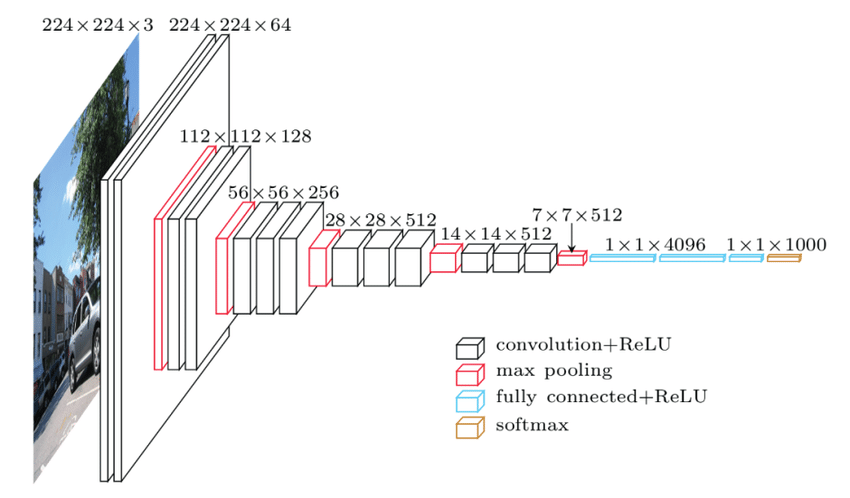
\includegraphics[width=.8\textwidth]{images/Chapter2/VGGNet-architecture-19.png}
\caption{Architecture of a VGG16 network. The input image is processed by 13 convolutions with a kernel size of 3x3. After the first two convolutions, a max pooling halves the resolution but doubles the amount of filters \citep{Bezdan_2019}.} 
\label{fig:vgg16}
\end{figure}

The 2015 introduced architecture for deep learning by the Visual Geometry Group of Oxford University (VGG) was one of the first networks that was able to get higher accuracies than shallower networks. \citet{Simonyan_2015} found out that two convolutions with a 3x3 kernel have the same field of view as one 5x5 kernel and three 3x3 kernels as one 7x7 respectively. The big improvement however was, that the number of parameters with three 3x3 kernels is considerably ($81\%$) lower than the number of parameters of one 7x7 kernel. This allows efficiency despite the network's depth. It is important to mention that this might come with possible disadvantages. Because of the change in kernel size, we might end up restricting our solution area. This will be neglected however, because it is not possible to test the two kernel sizes against each other. I will assume that the accuracy does not suffer from this effect.  Because VGG was developed for the ILSVRC which consists of 1000 classes, the convolution output is fed into two fully connected dense networks with 4096 channels each and a third and final dense network with 1000 outputs and a softmax activation function \eqref{softmax}. Softmax is another very common activation function, giving the probability of each output neuron and thus the probability for each of the 1000 image classes.

\begin{equation}
    f(\pmb{z})_i = \frac{e^{z_i}}{\sum_{j=1}^{K} e^{z_j}}, \; \;  \text{for} \; i=1 \; \; \text{and} \; \; \pmb{z} = (z_1,\ldots,z_K)
\label{softmax}
\end{equation}

The authors provide two different version of their network. VGG16 (\autoref{fig:vgg16}) consists of 16 total layers with 134 million parameters and VGG19 consists of 19 layers with 144 million parameters. For VGG19, the first two convolution layers are the same as for VGG16, but the next three have one additional convolution. The dense networks remain unchanged. The slightly deeper VGG19 was able to perform a little bit better than the shallower VGG16, scoring around $0.1\%$ less top-5 validation error thorughout multiple tests.
\subsubsection*{ResNet}
Only a year after VGG was introduced, \citet{He_2016} managed to develop a new method that allowed networks with depths of up to 152 layers to train more efficiently and predict more accurately than its predecessors. The way they were able to avoid the so called \textit{exploding gradient problem}, where the gradient is getting higher with every convolution and in consequence updating the weights more drastically resulting in an even higher gradient, is by introducing a new operation to deep learning: the \textit{residual}. \\

\begin{figure}[h!]
\centering
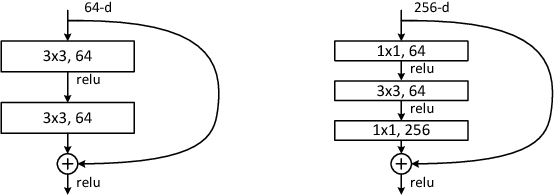
\includegraphics[width=.667\textwidth]{images/Chapter2/6-Figure5-1.png}
\caption{A residual block with two convolutions (\textit{left}) and three convolutions (\textit{right}). After the convolutions, the identity of the layer's input is added before an activation function and the next layer \citep{He_2016}.} 
\label{fig:resid}
\end{figure}

The main idea is to provide the deeper layers with information gathered before in order to not get lost in parameters the deeper the signal goes into the network. This is achieved by the identity function. After a convolutional layer, the identity from the last activation is added to the new activation,  allowing a massive improvement in network depth. The authors provide 34-(\autoref{fig:Res34}), 50-, 101- and 152-layer networks. The 34-layer network used the residual structure from \autoref{fig:resid} (\textit{left}) while the other architectures are based on the structure from \autoref{fig:resid} (\textit{right}). It's also worth noting that ResNet is not using dense nets at the end of the convolutional layers apart from the 1000 class dense net to receive probabilities for the image classification. It was shown that these fully connected layers were not needed for high accuracies and only increased the number of parameters unnecessarily. While the best VGG achieved a $6.8\%$ top-5 error rate in the 2015 ILSVRC, ResNet-34 already was beating this with a $5.6\%$ top-5 error. The deeper the network, the lower the error was and ResNet-152 was able to score an outstanding $3.57\%$ error, beating even human image classification with approximately $5.1\%$ top-5 error accuracy \citep{russakovsky2015imagenet}.


\subsubsection*{EfficientNet}
Finally, I want to take a closer look at a more recently developed architecture called EfficientNet. Its name indicates its goal, being more efficient than previous attempts. To achieve this, \citet{tan2020efficientnet} tried different scaling methods on a conventional deep network. 

\begin{figure}[h]
\centering
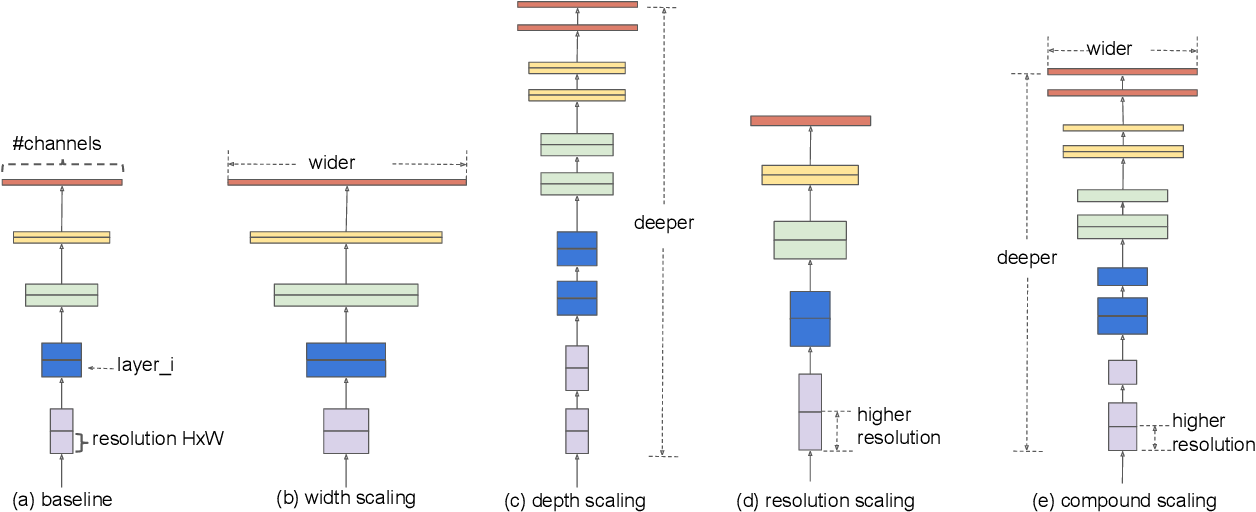
\includegraphics[width=\textwidth]{images/Chapter2/2-Figure2-1 (1).png}
\caption{Different scaling approaches for improving efficiency by keeping (or ideally improving) accuracy for deep learning architectures \citep{tan2020efficientnet}. } 
\label{fig:effnet_scaling}
\end{figure}

They chose three parameters to vary and optimize efficiency and accuracy along the way: the input resolution, the number of layers and the number of channels of each output. The latter is called width scaling, increasing the number of layers is depth scaling and changing the resolution is resolution scaling. A change of all parameters is referred to as compound scaling. They developed a neural network based on the approach by \citet{tan2019mnasnet} with a cost function that optimizes the amount of \textit{floating point operations per second} (FLOPS) by keeping a set accuracy, allowing them to develop a set of CNNs that achieve high accuracies with less operations and parameters needed in training. EfficientNet-B7, which I will use in training, has 66 million parameters, only six million more than the 60 million of ResNet152 by being significantly more accurate (see \autoref{fig:effnet_params}). \\
This indicates that the future of image recognition and classification won't be developed by humans alone, but by algorithms searching for the best model for a certain task.

\begin{figure}[H]
\centering
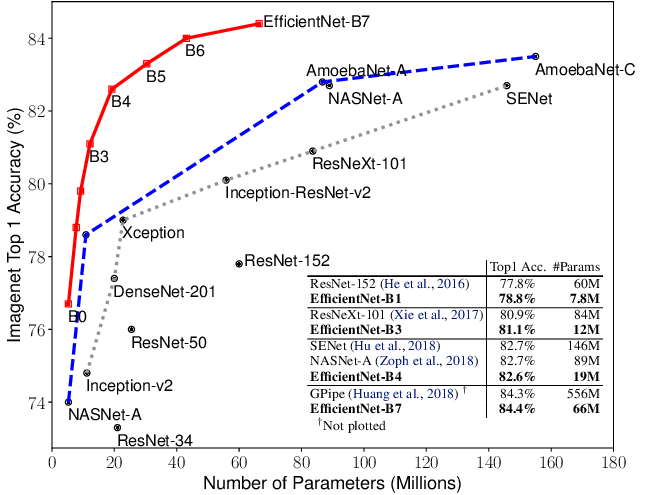
\includegraphics[width=.5\textwidth]{images/Chapter2/1-Figure1-1.png}
\caption{Comparison between the accuracy and number of parameters of EfficientNets and other successful CNN models \citep{tan2020efficientnet}. } 
\label{fig:effnet_params}
\end{figure}

After this brief introduction to the architectures used in my thesis, I want to talk about the implementation of them and the data that they will be provided with in training. 


\newpage

\section{Training the Neural Network}
\label{training}
The seemingly easiest part of developing a neural network can be the most challenging. Instead of sitting in front of the screen, watching epochs after epochs train while the loss keeps on decreasing, one is often puzzled by bad performing networks, overfitting and many more issues. The fact that neural networks will not provide any hint in why they fail makes the training part maybe the most important and least straightforward step towards useful predictions. This chapter is supposed to explain my training pipeline and the hurdles I had to overcome.
\subsection{The Data Catalogue}
\label{data_catalogue}
As mentioned in \cref{new_approach}, for many space observatories, there are simulations being made to have an insight into the data the instrument will produce. This data is perfect for training because it provides many different parameters to be evaluated from the telescopes output and knowing exactly how the simulations are produced, one knows to which extend the data is accurate compared to real-life observation data. \\
eROSITA is an X-Ray telescope developed by the \textit{Max Planck Institute for Extraterrestrial Physics} (MPE) and is part of the german-russion space-observatory \textit{Spektr-RG}. Among its goals was to create a sky survey in a frequency between $\sim 0.2\text{keV}$ and $\sim 8.0\text{keV}$ over a $\sim 140$ square degree area. This survey is called \textit{eROSITA Final Equatorial Depth Survey} or eFEDS for short. I will be using the data generated for this specific survey in order to infer galaxy cluster masses. The data given is centered on a galaxy cluster with a given mass and redshift. The image consists of an array of 50x50 pixels with ten frequency bands.

\begin{table*}[h]
\centering
\begin{tabular}{@{}cc@{}}\toprule
Frequency Band & Photon Energy $[\text{eV}]$ \\
\midrule
1 & $250-455$ \\
2 & $455-660$ \\
3 & $660-865$ \\
4 & $865-1070$ \\
5 & $1070-1275$ \\
6 & $1275-1480$ \\
7 & $1480-1685$ \\
8 & $1685-1890$ \\
9 & $1890-2095$ \\
10 & $2095-2300$ \\
\bottomrule
\end{tabular}
\caption{The ten frequency bands of the galaxy cluster images used for training.}
\label{tab:freq_bands}
\end{table*}





These frequencies are chosen for galaxy mass estimation, because they include the main spectrum for clusters with $T<10^8\text{K}$ (see \autoref{fig:x-ray_emission_curves}). This is confirmed by inspecting the image data for the highest energies from $1685 - 2300 \text{eV}$ (see \autoref{fig:cluster_big_freq}) because the galaxy cluster features are being less present there. In total, there are $7946$ galaxy clusters with each cluster being provided with a mass $\log{(M_{500}^{\text{true}}/M_{\odot})}$ where $M_{500}^{\text{true}}$ is the galaxy cluster mass for a virial density of 500 times the critical density of the universe and $M_{\odot}$ is the solar mass. Clusters with a mass $(13 < \log{(M_{500}^{\text{true}}/M_{\odot})} < 15)$ and redshift range of $(0.01 < z < 1.5)$ are chosen specifically because they proved successful in previous attempts \citep{Ntampaka_2018}.

\begin{figure}[H]
\centering
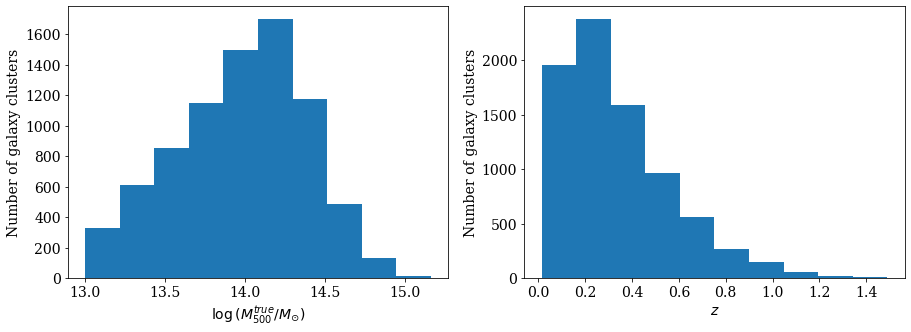
\includegraphics[width=\textwidth]{images/Chapter3/distr_data.png}
\caption{Distribution of the given galaxy cluster data. The mass distribution (\textit{left}) is roughly a normal distribution with a slight shift towards higher masses. The redshift (\textit{right}) is highly shifted towards smaller redshifts, meaning there are way more galaxy clusters with a shorter distance to Earth than clusters with greater distances.} 
\label{fig:data_dist}
\end{figure}

The actual galaxy cluster images do vary quite a bit in appearance. While there are galaxy clusters with a very obvious round or elliptical form (see \autoref{fig:cluster_big}), there are also clusters that are barely distinguishable from the background noise (see \autoref{fig:cluster_small}). In most cases the latter are either very small or far away while the opposite is true for galaxy clusters easily detectable with human-eye.

\begin{figure}[H]
\centering
\begin{subfigure}{.4\textwidth}
  \centering
  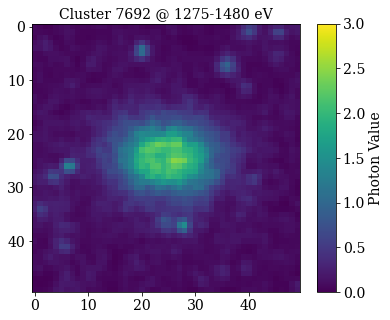
\includegraphics[width=\linewidth]{images/Chapter3/cluster_big.png}
  \caption{Galaxy cluster with a mass of $\log{(M_{500}^{\text{true}}/M_{\odot})} \approx 14.82$ at a redshift of $z \approx 0.12$}
  \label{fig:cluster_big}
\end{subfigure}%
\hspace{3.6em}
\begin{subfigure}{.4\textwidth}
  \centering
  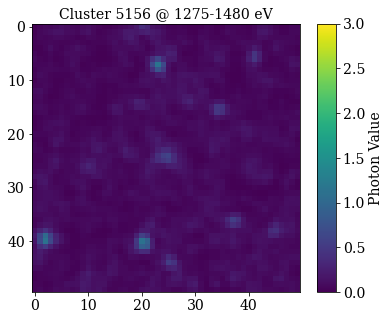
\includegraphics[width=\linewidth]{images/Chapter3/cluster_small.png}
  \caption{Galaxy cluster with a mass of $\log{(M_{500}^{\text{true}}/M_{\odot})} \approx 14.18$ at a redshift of $z \approx 0.3$}
  \label{fig:cluster_small}
\end{subfigure}
\caption{Two very different looking galaxy clusters at the same frequency band of $1275-1480 \text{eV}$ from the eFEDS simulation catalogue. The photon value is capped at three for easier visualisation.} 
\label{fig:cluster_comp}
\end{figure}


\begin{figure}[H]

\subfloat{%
  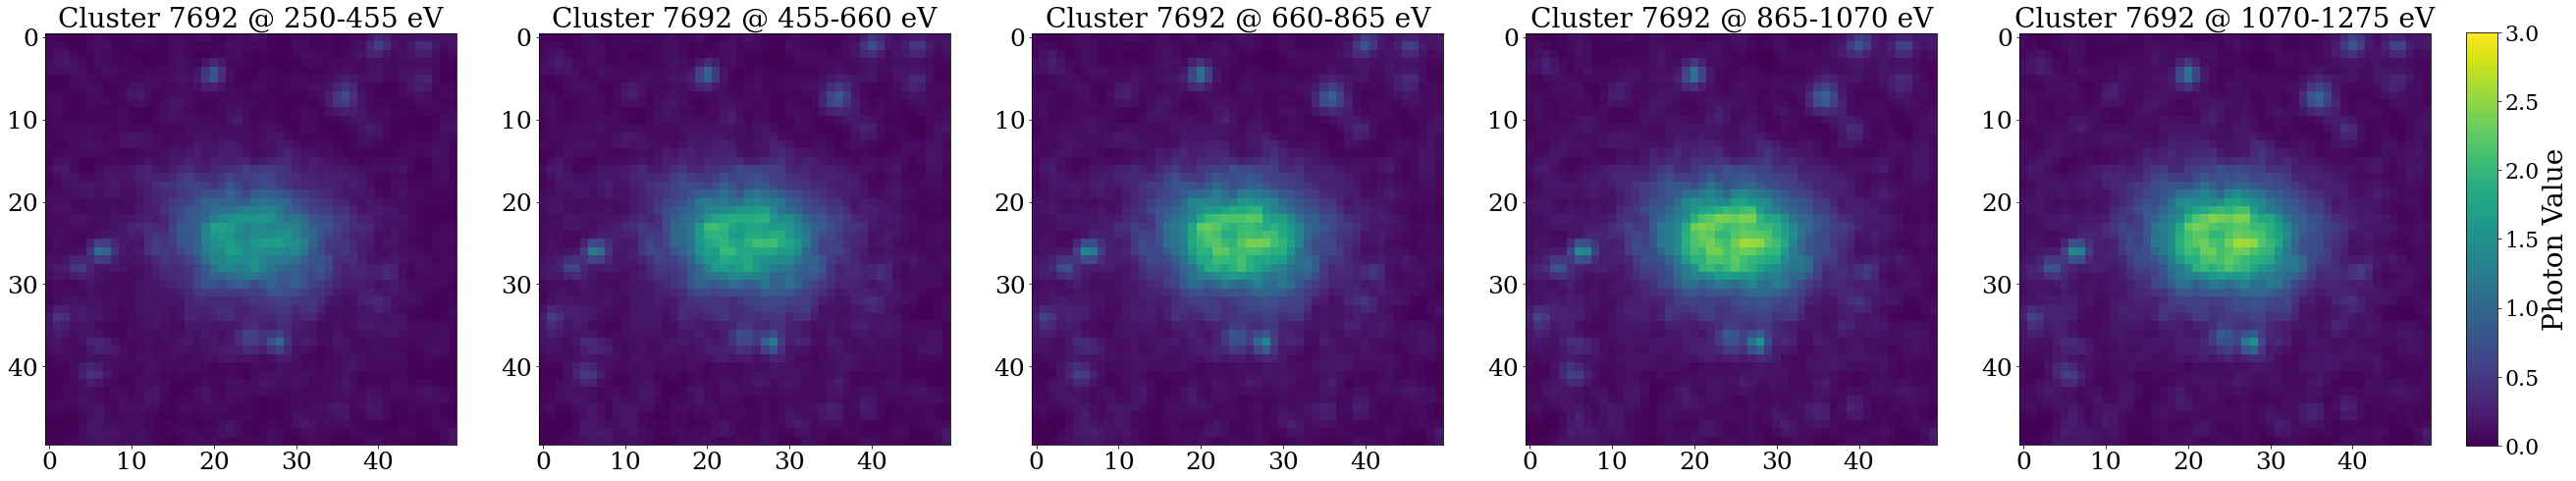
\includegraphics[clip,width=\columnwidth]{images/Chapter3/cluster_7692.png}%
}
\vspace{1em}
\subfloat{%
  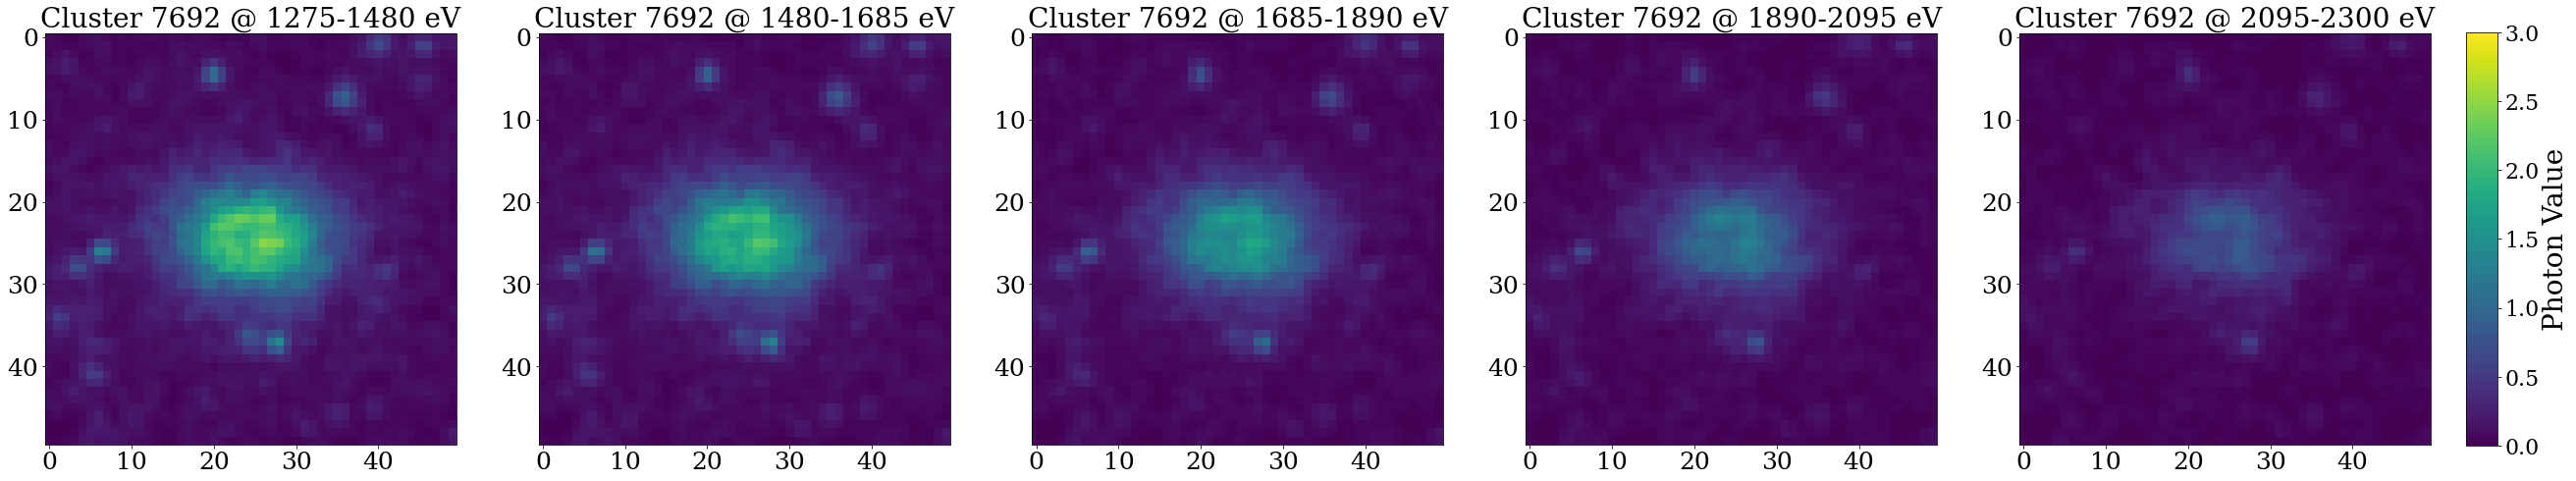
\includegraphics[clip,width=\columnwidth]{images/Chapter3/cluster_7692_II.png}%
}

\caption{All ten frequency bands for the galaxy from \autoref{fig:cluster_big}. Especially for higher frequencies, less photons are captured. Because of this, only frequencies up to $2300\text{eV}$ are being considered for mass estimation.}
\label{fig:cluster_big_freq}

\end{figure}

\subsection{Preparation of the Data}
\label{data_prep}
Before every training, the data must be carefully inspected and in most cases preselected and modified in order to efficiently train a neural network and avoid training issues such as overfitting and divergence.
To address these problems, we first have to split our data into two different sets, the \textit{training set} and \textit{test set}. If we were to use all of our data for training, there would not be a way to estimate whether our predictions are overfitted or not, because the model has already seen all of the data in training. To solve this, it is common to take about ten percent of the dataset as test set without showing it to the neural network during training. If our model is overfitting the training data, meaning only adapting to individual features in the images but not certain features that define the mass of galaxy clusters, the predictions on the test set will be worse than the predictions on the training set. This way we can easily spot any overfitting problems. An even more efficient way to spot overfitting is by also using a \textit{validation set}. This is similar to the test set in that it is not used for training the neural network. The difference to the test set however is, that it is used during training to evaluate the model's performance, meaning we can see how our predictions perform on an unseen dataset. It is possible though not ideal to use the test set as validation set. The only downside of this method is, that if we optimize our network during training by changing parameters in order to increase validation set accuracy, we can run into overfitting again if we don't use separate test and validation sets. In my training I will use $90\%$ of the dataset as training set and the remaining $10\%$ as test set and validation set because I won't change parameters during training. The galaxy clusters are randomly selected for each set to avoid any bias in differing sets. However, to compare model accuracy, the same training and test sets are being used in every training. Otherwise it is possible to have easier or harder test sets for the model to evaluate which makes a comparison difficult.

\begin{table*}[h]
\centering
\begin{tabular}{@{}lr@{}}\toprule
\textbf{Dataset} & \textbf{Entries} \\
\midrule
Complete Set & $7946$ \\
Training Set & $7151$ \\
Test/Validation Set & $795$ \\
\bottomrule
\end{tabular}
\caption{Number of entries for the complete-, training-, test- and validation set of galaxy clusters.}
\label{tab:freq_bands}
\end{table*}

Ready-made models sometimes need a certain input format for training. ResNet for instance needs at least 71x71 pixels of image input to train. Moreover, it is not possible to provide it with more than three frequencies because it was developed to train with color images consisting of three channels, red, green and blue (RGB). To be able to train anyways, some changes to our dataset are needed. Firstly, a padding of 21x21 pixels is added to the images. With this we achieve the desired image size of 71x71 pixels (see \autoref{fig:cluster_comp_padded}). For the sake of comparison, I also provided the basic network with only three frequencies despite it being able to train on all ten (as used in \citet{Krippendorf_2023}). Next, we have to select three of our ten frequency bands to train with. I decided to use the frequency range ($455\text{eV} < \nu < 1070\text{eV}$) because it allowed to see features for both smaller and bigger galaxy clusters. 


\begin{figure}[H]
\centering
\begin{subfigure}{.4\textwidth}
  \centering
  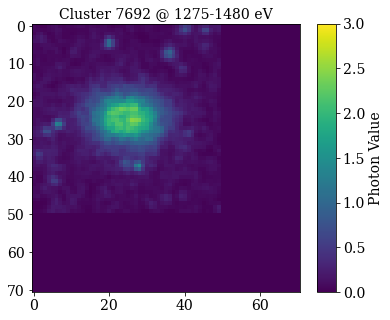
\includegraphics[width=\linewidth]{images/Chapter3/cluster_big_padded.png}
  \label{fig:cluster_big_padded}
\end{subfigure}%
\hspace{3.6em}
\begin{subfigure}{.4\textwidth}
  \centering
  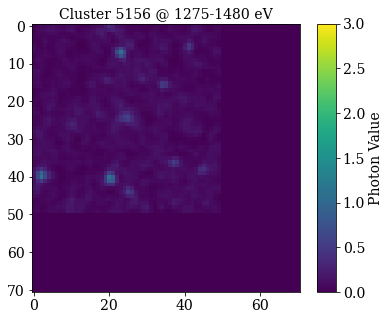
\includegraphics[width=\linewidth]{images/Chapter3/cluster_small_padded.png}
  \label{fig:cluster_small_padded}
\end{subfigure}
\caption{Galaxy clusters from \autoref{fig:cluster_comp} with the added padding of 21x21 pixels for training with deep models.} 
\label{fig:cluster_comp_padded}
\end{figure}

The final step before training is another randomization of our data. This helps to avoid any bias that our dataset already includes. There could be for example a bias in the way the simulation generates galaxy clusters, preferring a certain rotation. Because there is no designated direction in space, we expect galaxy clusters to be randomly rotated. Because of that, a random flip of each galaxy cluster image is performed before training.
This gives us the full data preparation pipeline as seen in \autoref{fig:pipeline}.

\begin{figure}[H]
\centering
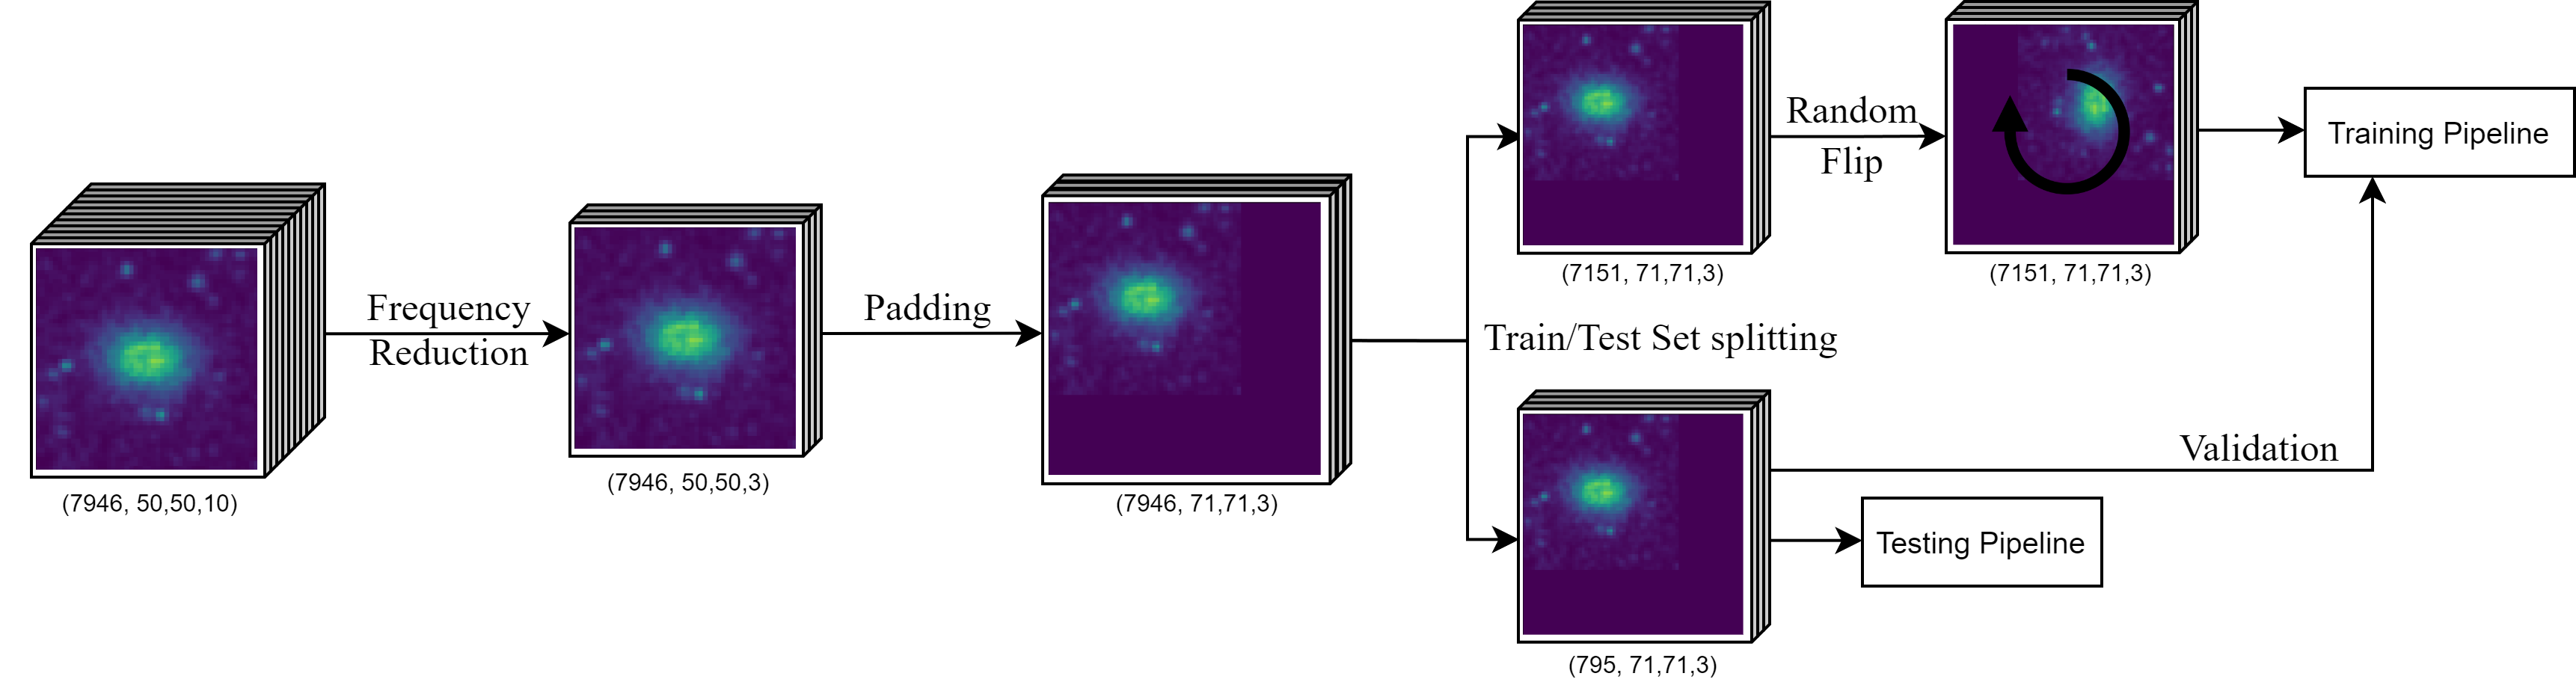
\includegraphics[width=\linewidth]{images/Chapter3/pipeline.png}
\caption{Full data preparation pipeline. The numbers below each step stand for (samples,x-image size,y-image size,frequencies)} 
\label{fig:pipeline}
\end{figure}
\subsection{Training Parameters}
\label{train_params}
To get an idea of the different model depths, consider \autoref{tab:model_params}. The deeper models have considerably more parameters that can be varied in training. As discussed in \cref{basic_cnn}, the neural network performs a gradient descent to minimize the loss function. The more parameters it can vary, the more difficult it is to keep a balance between the learning rate $\alpha$ and problems with overfitting. This means, that the more complex the network gets, the harder it is to optimize it.


\begin{table*}[h]
\centering
\begin{tabular}{@{}ccc@{}}\toprule
Model Name & Parameters $[\text{Million}]$ & Time per Epoch [sec] \\
\midrule
Basic CNN & $0.30$ & $<1$\\
VGG16 & $15.76$ & $6$\\
VGG19 & $21.07$ & $5$\\
ResNet50 & $32.97$ & $7$\\
ResNet50V2 & $32.95$ & $6$\\
ResNet101 & $51.99$ & $12$\\
ResNet101V2 & $51.97$ & $10$\\
ResNet152 & $67.66$ & $17$\\
ResNet152V2 & $67.63$ & $16$\\
EfficientNet-B7 & $21.07$ & $23$\\
\bottomrule
\end{tabular}
\caption{Trainable parameters of the chosen models for training and training time for training on a GPU.}
\label{tab:model_params}
\end{table*}

The first training parameter I want to discuss is the \textit{pretraining}. For the deep models there is an option that allows you to download and use a model that has already been training on different training sets. For example you can choose to use a model already trained on ImageNet images. This has the advantage that you don't have to train the network in order for it to learn helpful filters like edge detection, which can help to increase training efficiency. I decided to choose the imagenet pretraining weights to help with training speeds. The pretrained information are obtained simply by downloading the weights that the model has learned in previous training. \\

As \textit{loss function} I use the mean squared error (MSE) \eqref{MSE}. It is the standard loss function for almost all neural network applications and should work fine with our models.

Next, we have to chose an \textit{optimizer} that will help us perform the gradient decent in an efficient way. I chose the most popular optimizer called Adaptive Moment Estimation (Adam) \citep{kingma2017adam}. Its advantage is, that it tracks the previous steps of the gradient decent for every parameter and then changes the learning rate accordingly for every parameter to reduce overfitting. It's given a baseline stepsize (\textit{learning rate}) to change the gradient decent speed with which it is going towards the minimum. The standard value is $0.001$ and I kept this for every training to maintain comparability. Ideally, one would change this value for every model and see the effects it has on overfitting and overall accuracy. I will further discuss this in the results for the basic CNN in \cref{res_basic_cnn}.\\

While some architectures like VGG use dense networks at the end of the convolutional block, others like ResNet don't. Despite that, after providing the additional redshift information, I always use another dense network to also learn the effect of the redshift combined with the already learned features of the image. For this I use a dense network with $512$ neurons. Only the basic CNN varies with two dense networks with 100 neurons each to stick to the architecture used by \citet{Krippendorf_2023}. As mentioned in \cref{basic_cnn}, dense networks need activation functions for which I chose ReLU for its simplicity and effectiveness.\\

The last very important parameter for training is the amount of cycles the model has to train for. Normally, the data is being fed into the training processes in \textit{batch sizes}, meaning only a certain amount of data at a time. Using thousands of samples, high batch sizes could fill up the computer's memory fairly quickly while small batch sizes would train too slowly. I decided to train with a batch size of 32 which is the standard for neural network training. Each run through a single batch is called iteration. One \textit{epoch} is a full cycle trough all of the data. Choosing a suitable number of epochs is quite difficult because it depends strongly on all the other parameters. If the learning rate is very small, more epochs are needed to reach a certain level of training and vice versa. For the deep models I chose 4000 epochs while the basic CNN is only trained for a few hundred epochs before running into overfitting (see \cref{res_basic_cnn}). I decided to use 4000 epochs as a compromise between training for accuracy and overall training time (see \autoref{tab:model_params}). Especially ResNet sometimes picked up certain features after a few thousand epochs of training (see \cref{res_ResNet}). Because of that, 4000 seemed like a good compromise for it to train well.


\begin{table*}[h]
\centering
\begin{tabular}{@{}cc@{}}\toprule
Parameter & Chosen Setting \\
\midrule
Pretraining* (training catalogue) & Yes (Imagenet) \\
Loss Function & MSE \\
Optimizer & Adam \\
Learning Rate & 0.001 \\
Dense Units* & $512$ \\
Dense Activation & ReLU \\
Batch Size & 32 \\
Training Epochs* & 4000 \\
\bottomrule
\end{tabular}
\caption{Chosen settings for training the different deep models. \\ *There is no pretraining for the basic CNN and the number of dense units is chosen as discussed in \cref{basic_cnn}. The number of epochs for the basic CNN is varied to see the effects of overfitting and different learning rates in \cref{res_basic_cnn}.}
\label{tab:model_settings}
\end{table*}



\newpage

\section{Results}
\label{Results}
Neural network training can sometimes be tedious and often one gets completely different results for the same parameters chosen. To address the randomness of some training successes and failures, I trained every model ten times. Thus I will provide some training insights about what I noticed within these ten runs and more importantly I will show and examine the strongest model of each run in detail. The used graphs and figures are explained in detail for the basic CNN in \cref{res_basic_cnn} in order to explain problems like overfitting and the effect of different learning rates. For the deep models, I will show the exact same graphs for comparison. After the individual results, I will discuss and compare the complete results in \cref{Results}.\\
To evaluate the performance of the model's predictions apart from the plots, I use the standard deviation

\begin{equation}
    \sigma = \sqrt{\frac{\sum_{i=1}^{n}(\|x_i\| - \Tilde{\mu})^2}{n}},
\end{equation}

where $x_i$ is the difference between the model predictions and the true masses

\begin{equation}
    x_i =(\log{(M_{500}^{\text{NN}}/M_{\odot})} - \log{(M_{500}^{\text{true}}/M_{\odot})})_i
\end{equation}

and the expected value

\begin{equation}
    \Tilde{\mu} = \frac{\sum_{i=1}^{n}\|x_i\|}{n},
\end{equation}

where $n$ is the number of predictions.

I use another expected value $\mu$ without the absolute value of the difference between the predicted and the true mass

\begin{equation}
    \mu = \frac{\sum_{i=1}^{n} x_i}{n}.
\end{equation}

This allowes me to not only see the average difference between the two values, but also whether the predictions are too high ($\mu < 0$) or too low ($\mu > 0$).
The standard deviation gives a measure of the spread of the models predictions. A model with a high $\sigma$ has a larger spread in predictions than a model with a small $\sigma$.

\subsection{The Basic CNN (Baseline)}
\label{res_basic_cnn}
\subsubsection*{Training Insights}


As mentioned in \cref{train_params}, I decided to not use 4000 epochs of training for the basic network. To explain why, consider \autoref{fig:basic_cnn_overf}. This plot shows the training history for the basic model and the previously mentioned training parameters. The validation loss has a minimum after just 90 epochs of training and keeps on rising until reaching a steady level for the rest of the training. The training loss though keeps on decreasing for the whole training. This indicates that the model reached a certain amount of accuracy quickly but as training progressed, it started to overfit the individual images and accuracy on the validation set decreased. 

\begin{figure}[H]
\centering
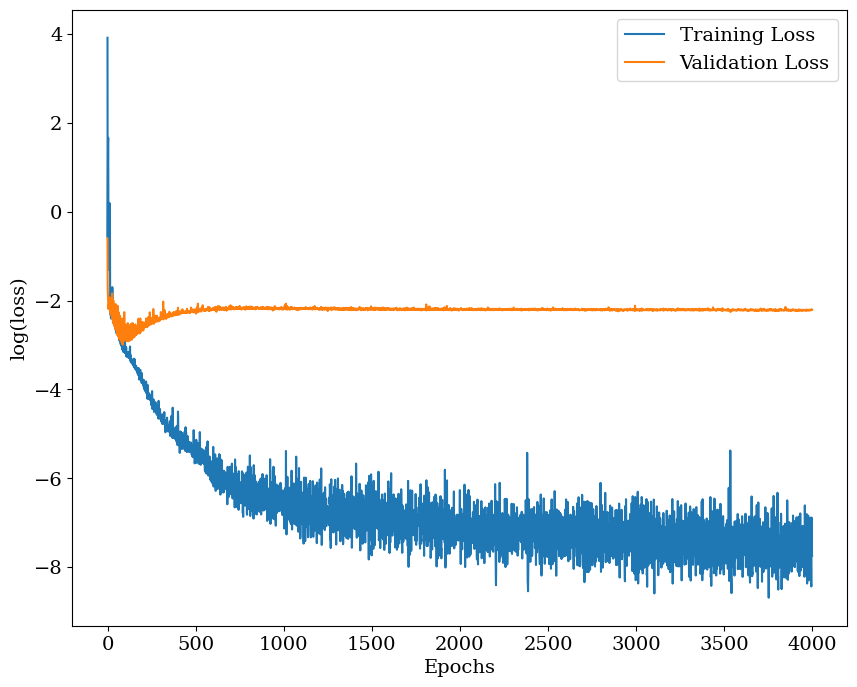
\includegraphics[width=.667\textwidth]{images/Chapter4/Basic CNN/hist_overf.png}
\caption{Training history for the basic CNN model. While the training loss is continuously getting lower, the validation loss reached its minimum after around 100 epochs, indicating overfitting. The validation loss reached a value of 0.130 and the training loss of 0.0006 after 4000 epochs of training.} 
\label{fig:basic_cnn_overf}
\end{figure}

We would expect the predictions on the test set to be way worse than the predictions on the training set. To examine this, consider \autoref{fig:overf_comp} and \ref{fig:overf_comp_hist}.

\begin{figure}[H]
\centering
\begin{subfigure}{.46\textwidth}
  \centering
  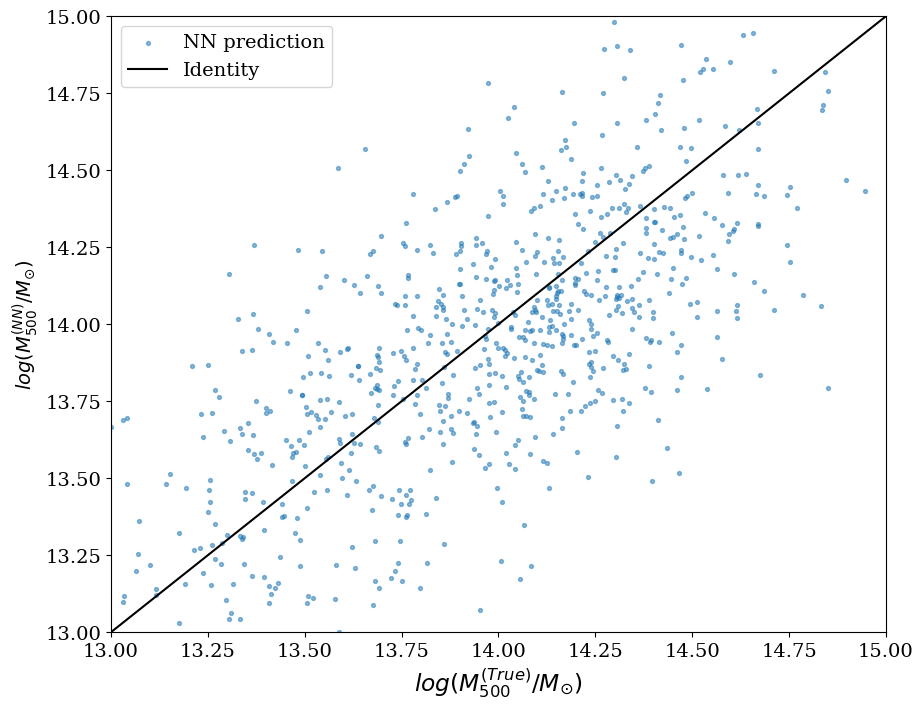
\includegraphics[width=\linewidth]{images/Chapter4/Basic CNN/overf_test_set.png}
  \caption{Model predictions on the test set.}
  \label{fig:overf_comp_test}
\end{subfigure}%
\hspace{.6em}
\begin{subfigure}{.46\textwidth}
  \centering
  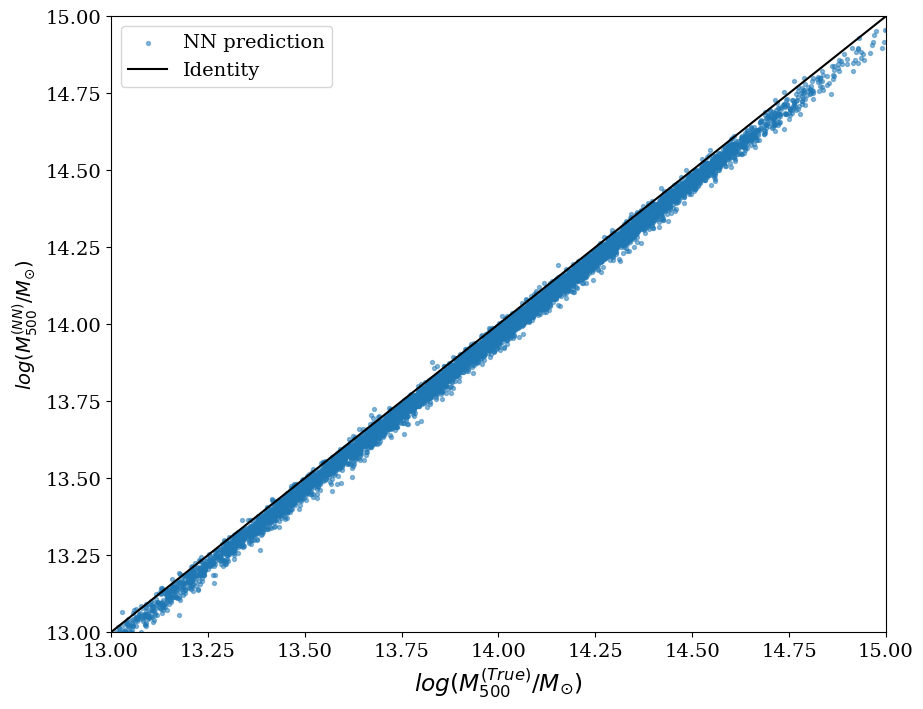
\includegraphics[width=\linewidth]{images/Chapter4/Basic CNN/overf_test_trainset.png}
  \caption{Model predictions on the training set.}
  \label{fig:overf_comp_train}
\end{subfigure}
\caption{Difference between the test and the training predictions of the trained model. The x-axis shows the true mass and the y-axis the predicted mass. The very exact predictions on the training set indicate overfitting which is confirmed by the bad predictions on the test set.} 
\label{fig:overf_comp}
\end{figure}

\begin{figure}[H]
\centering
\begin{subfigure}{.46\textwidth}
  \centering
  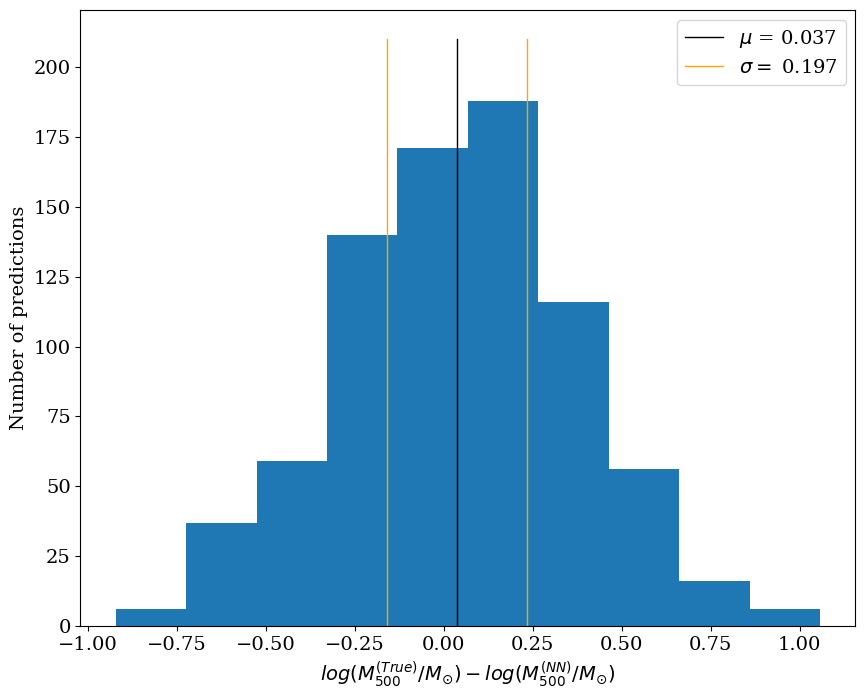
\includegraphics[width=\linewidth]{images/Chapter4/Basic CNN/overf_test_set_hist.png}
  \caption{Histogram of model predictions on the test set.}
  \label{fig:overf_comp_test_hist}
\end{subfigure}%
\hspace{.6em}
\begin{subfigure}{.46\textwidth}
  \centering
  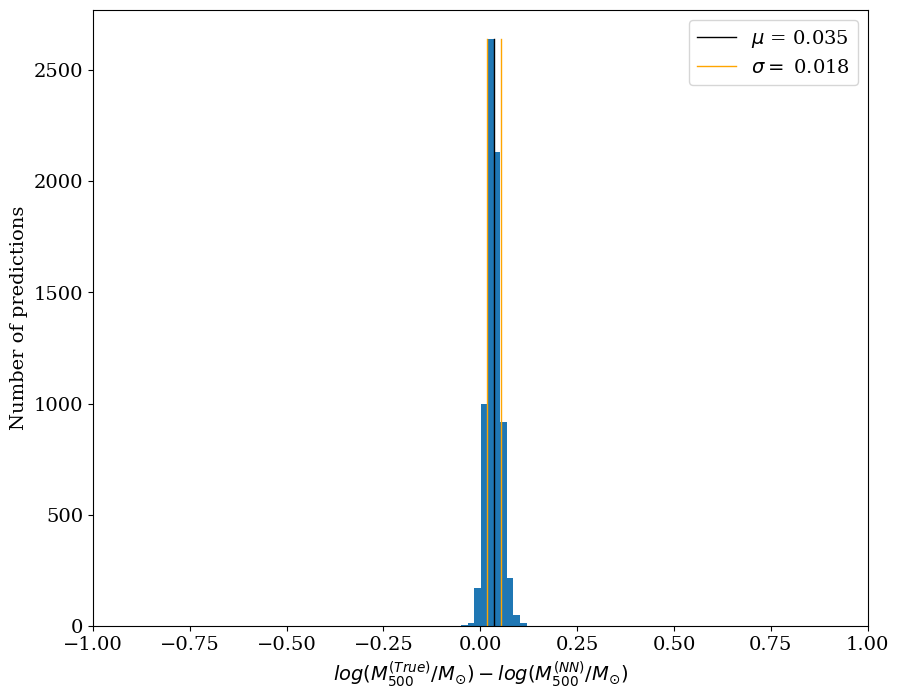
\includegraphics[width=\linewidth]{images/Chapter4/Basic CNN/overf_train_set_hist.png}
  \caption{Histogram of model predictions on the training set.}
  \label{fig:overf_comp_train_hist}
\end{subfigure}
\caption{Looking at the difference between the actual mass an the predicted mass, it is easy to spot the overfitting. It also indicates that the model is predicting somewhat smaller than the actual masses.} 
\label{fig:overf_comp_hist}
\end{figure}

Knowing what overfitting looks like now, we can try to improve our training. There are countless ways to do that. One could stop the training earlier, for example at around 100 epochs where the validation loss was at a minimum. Another way would be to lower the learning rate. This allows the model to train more slowly and maybe find another solution to more accurate predictions that do not encourage overfitting. 

\begin{figure}[H]
\centering
\begin{subfigure}{.46\textwidth}
\centering
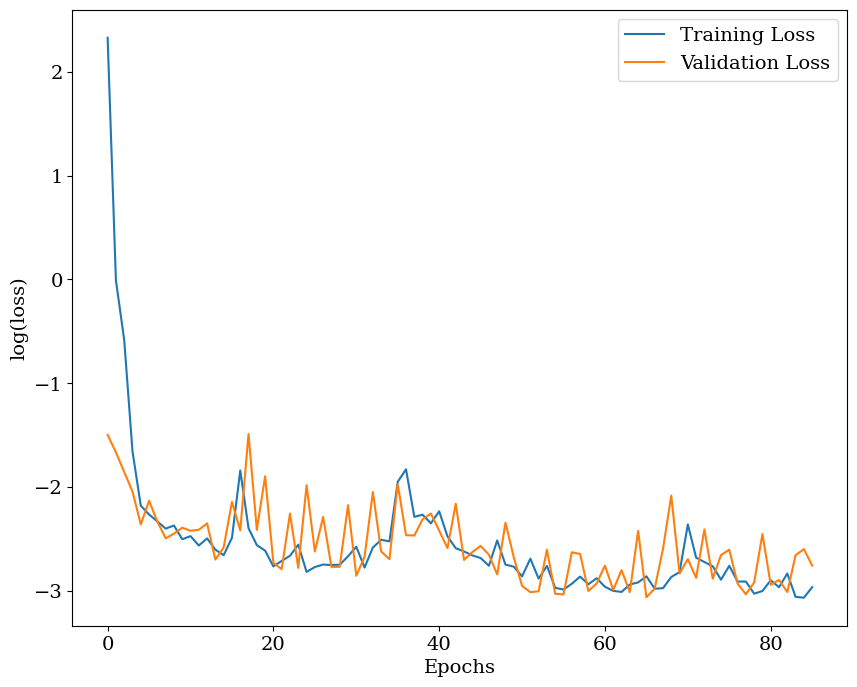
\includegraphics[width=\textwidth]{images/Chapter4/Basic CNN/best_perf_historie.png}
\caption{Training history for the best basic CNN model with a learning rate of 0.001, stopped after around 90 epochs.} 
\label{fig:comp_learning_rates_a}
\end{subfigure}
\hspace{.6em}
\begin{subfigure}{.46\textwidth}
\centering
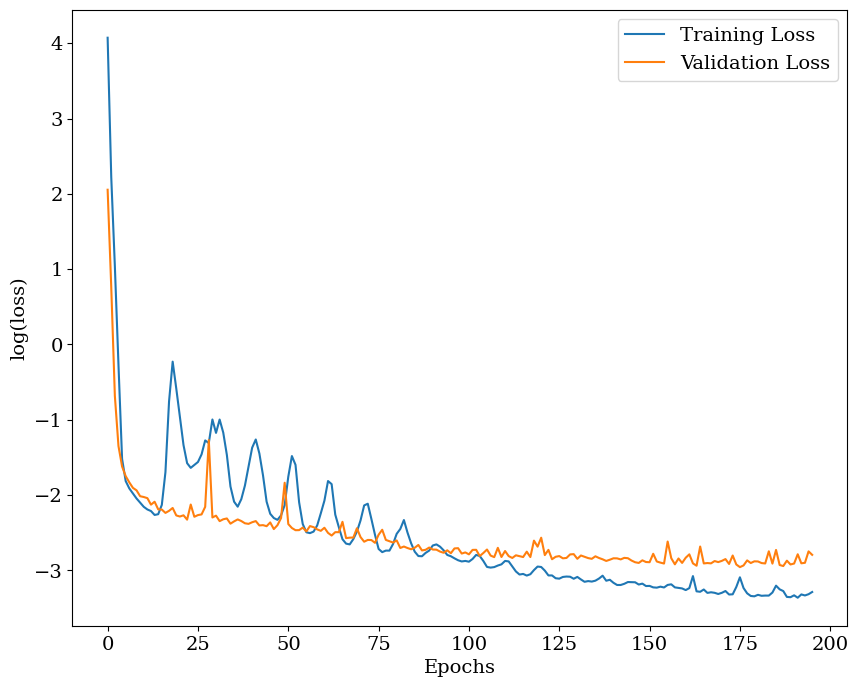
\includegraphics[width=\textwidth]{images/Chapter4/Basic CNN/hist_learning_rate.png}
\caption{Training history for the basic CNN model with a learning rate of 0.0005, stopped after around 190 epochs.} 
\label{fig:comp_learning_rates_b}
\end{subfigure}
\caption{A learning rate of $0.001$ (\textit{left}) compared to a learning rate of $0.0005$ (\textit{right}). The training with a lower learning rate reached its validation loss minimum after around double the epochs of the training with the standard learning rate of $0.001$.}
\label{fig:comp_learning_rates}
\end{figure}

There were no huge differences between these two approaches to prevent overfitting. The two shown trainings (\autoref{fig:comp_learning_rates}) produced similar results, with the standard learning rate (\autoref{fig:comp_learning_rates_a}) being a bit more accurate which could be due to training randomness. In more trainings, the slower learning rate could sometimes beat the standard learning rate. I decided to keep the standard learning rate and use a feature called \textit{early stopping} for the basic CNN. It keeps track of the validation loss and stops training as soon as it does not improve for a given amount of epochs. It is then possible to save the model with the lowest validation loss.

Let's take a look at what the predictions look like for stopping the training earlier:

\begin{figure}[H]
\centering
\begin{subfigure}{.46\textwidth}
  \centering
  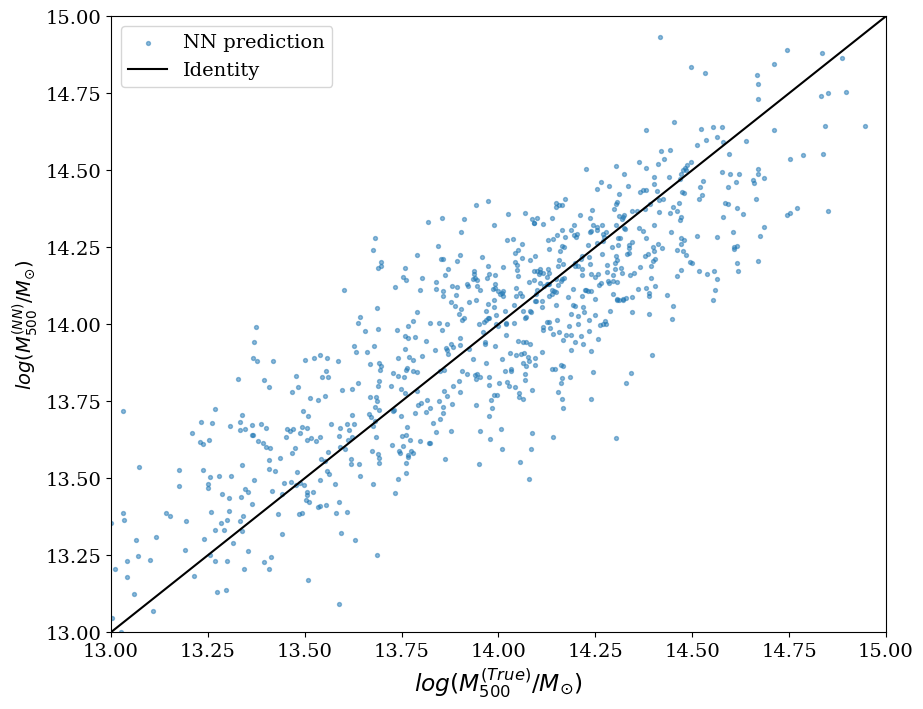
\includegraphics[width=\linewidth]{images/Chapter4/Basic CNN/best_perf_test.png}
  \caption{Model predictions on the test set.}
\end{subfigure}%
\hspace{.6em}
\begin{subfigure}{.46\textwidth}
  \centering
  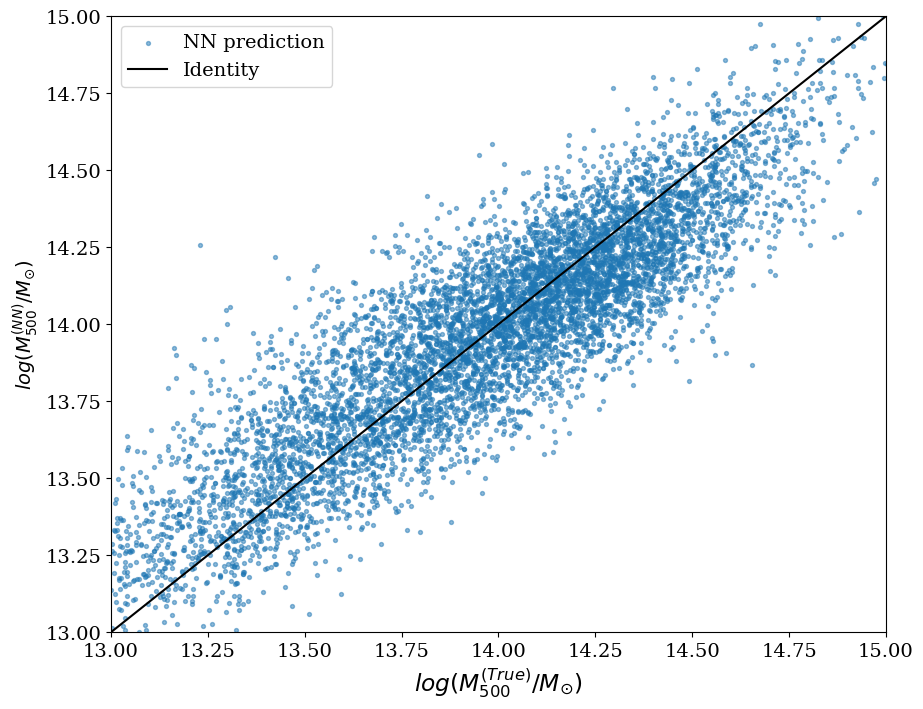
\includegraphics[width=\linewidth]{images/Chapter4/Basic CNN/best_perf_train.png}
  \caption{Model predictions on the training set.}
\end{subfigure}
\caption{Difference between the test and the training predictions of the trained model from \autoref{fig:comp_learning_rates_a}. This time the predictions on the test set are better than before (see \autoref{fig:overf_comp}) while the predictions on the training set are worse which indicates no, or only little overfitting.} 
\label{fig:short_training_comp}
\end{figure}

\begin{figure}[H]
\centering
\begin{subfigure}{.46\textwidth}
  \centering
  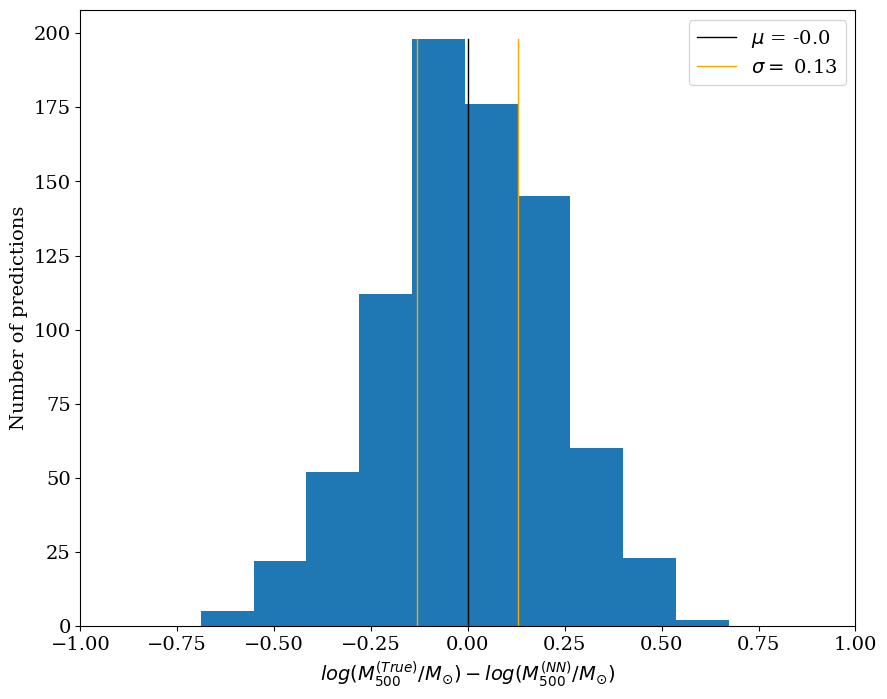
\includegraphics[width=\linewidth]{images/Chapter4/Basic CNN/best_perf_test_hist.png}
  \caption{Histogram of model predictions on the test set.}
\end{subfigure}%
\hspace{.6em}
\begin{subfigure}{.46\textwidth}
  \centering
  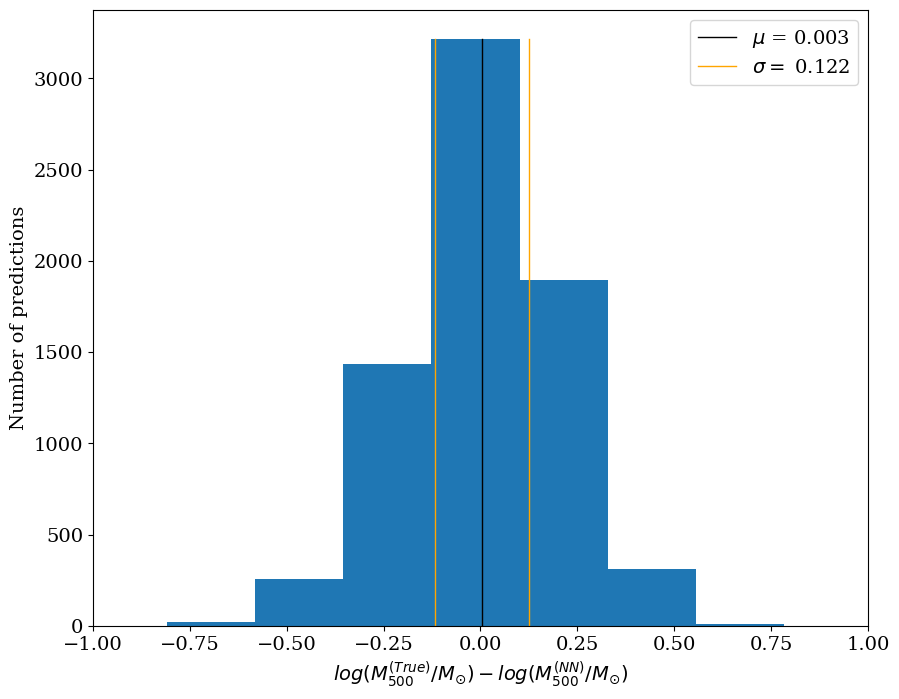
\includegraphics[width=\linewidth]{images/Chapter4/Basic CNN/best_perf_train_hist.png}
  \caption{Histogram of model predictions on the training set.}
\end{subfigure}
\caption{Now the histograms look way more similar to each other, which is exactly what we are looking for. This is also confirmed by the lower standard deviation of the difference between the actual and the predicted mass compared to the overfitted model.} 
\label{fig:short_training_comp_hist}
\end{figure}

For the basic CNN and for the deep models, I made a run of ten trainings each and will discuss their performance in the following sections starting with the best performing basic CNN.

\subsubsection*{Best Performing Model}

The best performing basic CNN reached its validation loss minimum after around 90 epochs of training. Compared to other trainings, it seemed to have picked up a useful filter early on as both the training and validation loss decrease significantly after only a few epochs. The predictions are nicely spread around the identity (see \autoref{fig:short_training_comp}) and consequently the average $\mu$ of the difference between the true and the predicted value is almost zero.\\
It is worth noting that this is already an improved model with an improved number of epochs to avoid overfitting. Moreover, the model's parameters were chosen to work for the given task by \citet{Krippendorf_2023}. For the deep models, the amount of epochs is set to 4000 and no other optimizations is done. \\

Normally, one would try to avoid overfitting where possible. In our case though, it is fine if we will observe overfitting, because we want to investigate whether a model is able to predict galaxy cluster masses in any way. If a model is not even able to make decent predictions on the training set after a few thousand epochs of training, it won't be suitable for our goal while a model that overfits massively after the training is at least able to find features within the images and is worth taking a deeper look at and optimizing later on. Because of that I will solely focus on the training results after 4000 epochs of training without any optimization.



\subsection{VGG}

These are the results for the ten training runs of the two VGG models, VGG16 and VGG19 split up into two parts. The training insights are supposed to give information about certain features I witnessed during training, while the best performing model section takes a closer look at the best model from the ten training runs.

\subsubsection{VGG16}
\label{vgg_16_res}
\subsubsection*{Training Insights}
The VGG16 model seemed to struggle with estimation of the whole mass range. All of the trainings resulted in predictions that are cut of at a mass of around $\log{(M_{500}^{\text{true}}/M_{\odot})} \sim 14.3$. Moreover, some trainings have made good improvements early on but then suddenly made a step in the wrong direction and did not recover (see \autoref{fig:vgg_history}). Maybe a smaller learning rate could improve this in future attempts.

\subsubsection*{Best Performing Model}
\begin{figure}[H]
\centering
\begin{subfigure}{.46\textwidth}
\centering
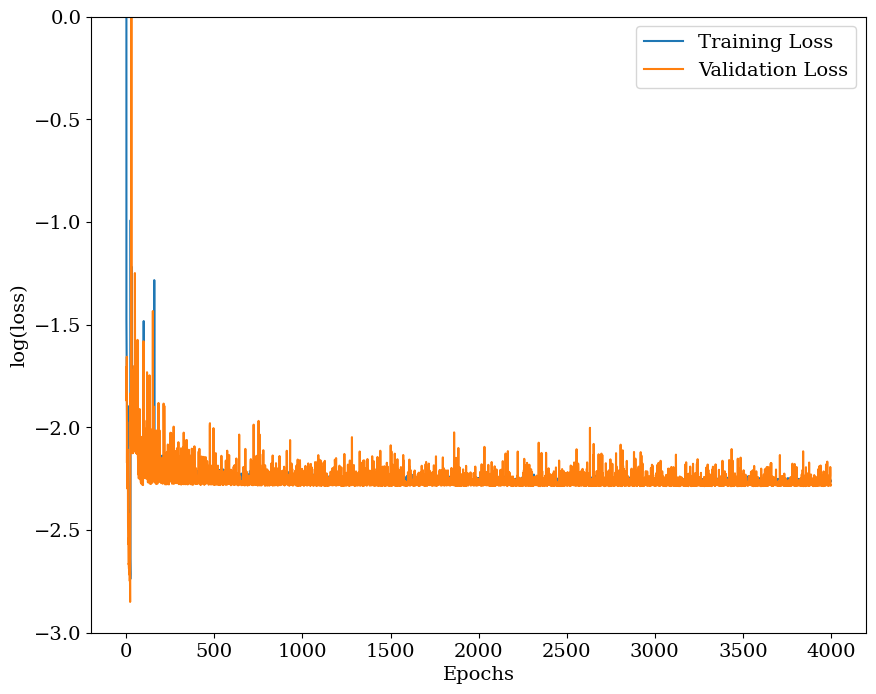
\includegraphics[width=\textwidth]{images/Chapter4/VGG16/vgg_history_full.png}
\caption{Full training history for VGG16 model.} 
\label{fig:vgg_history_a}
\end{subfigure}
\hspace{.6em}
\begin{subfigure}{.46\textwidth}
\centering
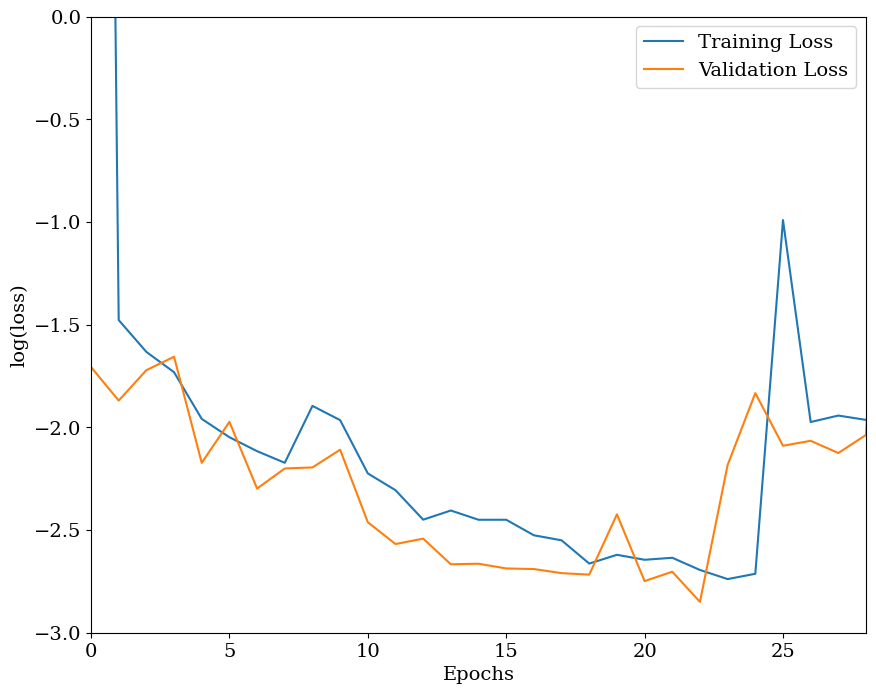
\includegraphics[width=\textwidth]{images/Chapter4/VGG16/vgg_history_zoom.png}
\caption{Zoom on the early dip.} 
\label{fig:vgg_history_b}
\end{subfigure}
\caption{Training history for the best performing VGG16 model. There is a dip very early after which the validation and training loss is considerable higher. In \autoref{fig:vgg_history_b}, a zoom on this dip is shown. The training loss is not developing at all after just a few epochs.}
\label{fig:vgg_history}
\end{figure}

Interestingly, the best performing VGG16 model started very strong by reducing the validation loss rapidly. For some reason tough, after around 25 epochs, the loss for both the validation and training set increased significantly and did not recover until the end of training. This shows that the model has difficulties finding anything useful in the provided images. Which is reflected in the bad predictions as well.

\begin{figure}[H]
\centering
\begin{subfigure}{.46\textwidth}
  \centering
  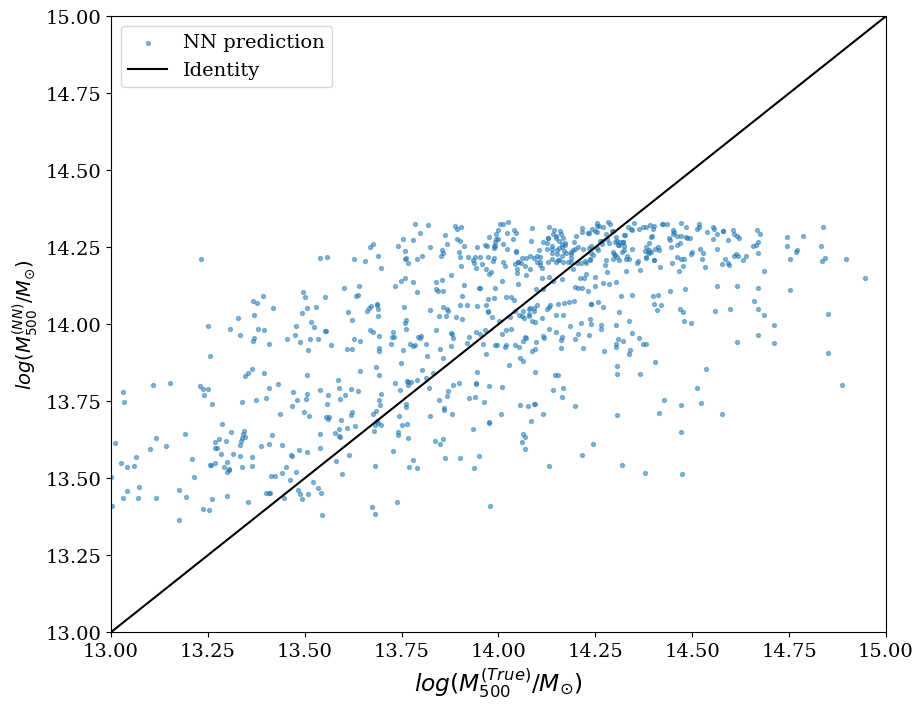
\includegraphics[width=\linewidth]{images/Chapter4/VGG16/vgg_pred_test.png}
  \caption{Model predictions on the test set.}
  \label{fig:best_perf_vgg16_a}
\end{subfigure}%
\hspace{.6em}
\begin{subfigure}{.46\textwidth}
  \centering
  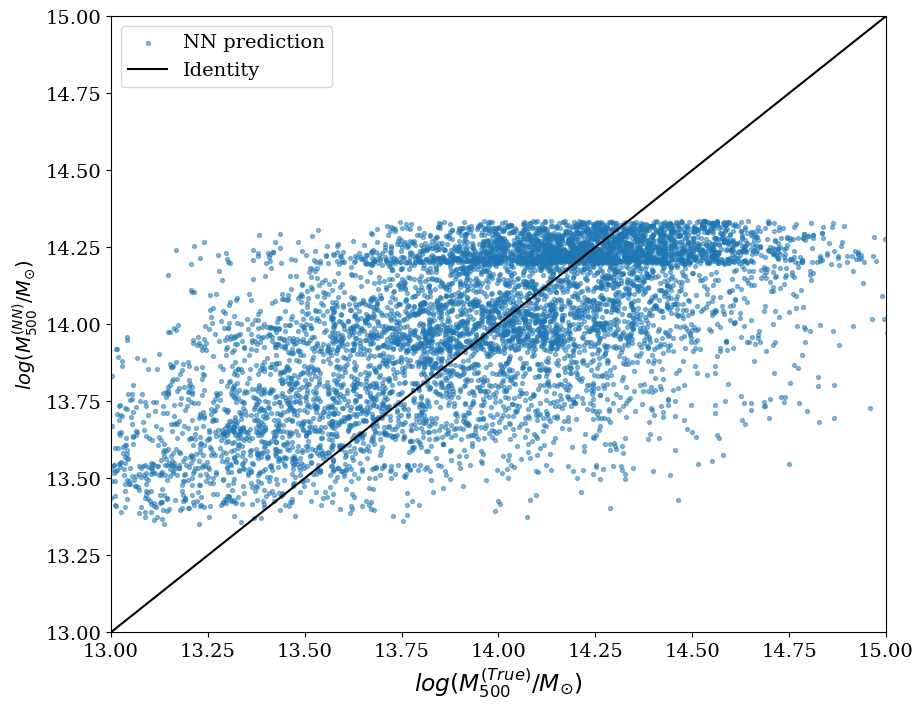
\includegraphics[width=\linewidth]{images/Chapter4/VGG16/vgg_pred_train.png}
  \caption{Model predictions on the training set.}
  \label{fig:best_perf_vgg16_b}
\end{subfigure}
\begin{subfigure}{.46\textwidth}
  \centering
  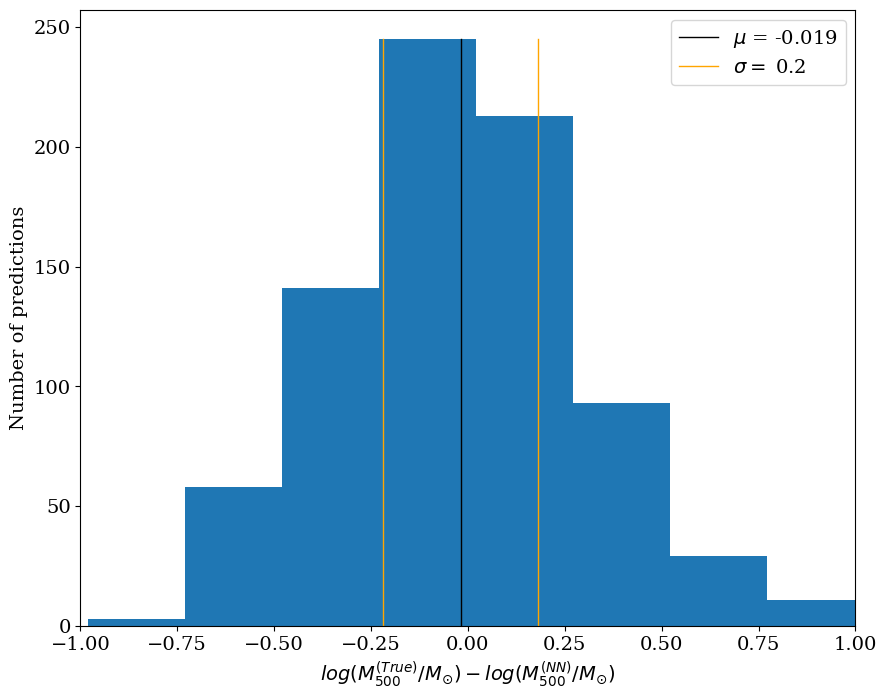
\includegraphics[width=\linewidth]{images/Chapter4/VGG16/vgg_pred_test_hist.png}
  \caption{Histogram of model predictions on the test set.}
  \label{fig:best_perf_vgg16_c}
\end{subfigure}%
\hspace{.6em}
\begin{subfigure}{.46\textwidth}
  \centering
  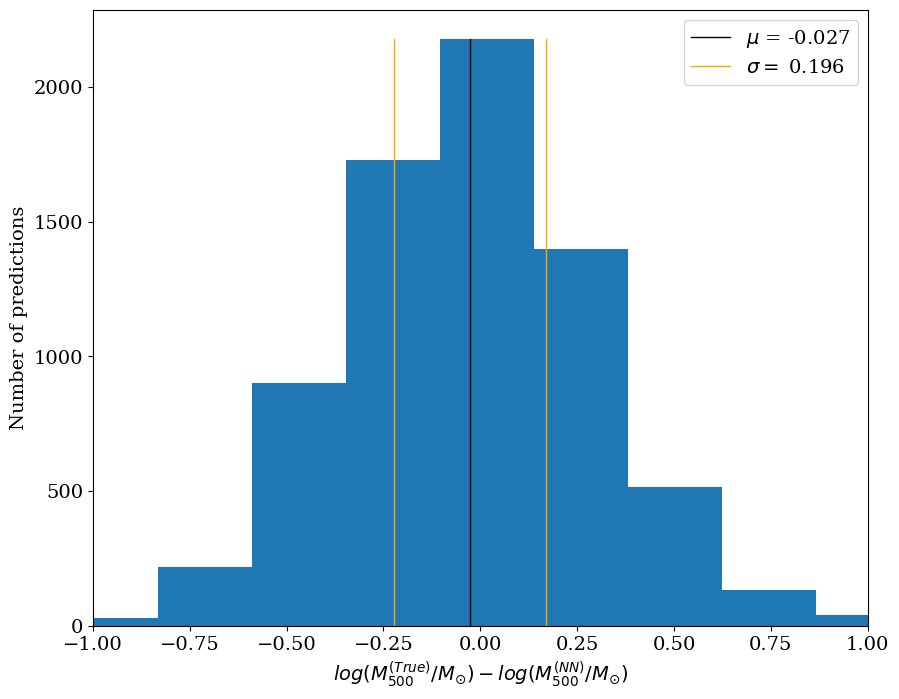
\includegraphics[width=\linewidth]{images/Chapter4/VGG16/vgg_pred_train_hist.png}
  \caption{Histogram of model predictions on the training set.}
  \label{fig:best_perf_vgg16_d}
\end{subfigure}
\caption{Prediction analysis for VGG16 model. This model struggled to achive good predictions. It did not predict any value above a mass of $\log{(M_{500}^{\text{true}}/M_{\odot})} \sim 14.4$. } 
\label{fig:best_perf_vgg16}
\end{figure}

The best model does not seem to overfit the training data. Nevertheless, the predictions are widely spread and there are even some horizontal lines visible within the predictions where the model seemed to predict a certain value for many different galaxy clusters (e.g. at masses around $\log{(M_{500}^{\text{true}}/M_{\odot})} = 13.9$ and $\log{(M_{500}^{\text{true}}/M_{\odot})} = 14.25$). I have seen this behaviour from all trained VGG16 models and do not yet understand the origin of this.


\subsubsection{VGG19}
\subsubsection*{Training Insights}
Training the VGG19 model was not very different from the VGG16 model. It also struggled to predict values above a mass of $\log{(M_{500}^{\text{true}}/M_{\odot})} \sim 14.3$ and the predictions are widely spread throughout the mass range. Even the best model did not produce useful predictions for galaxy mass estimations.


\subsubsection*{Best Performing Model}
The best performing VGG19 model did not perform very well. Its results are very similar to the ones from the best performing VGG16 model with similar $\sigma$ and $\mu$ values on both the test and training set.

\begin{figure}[h]
\centering
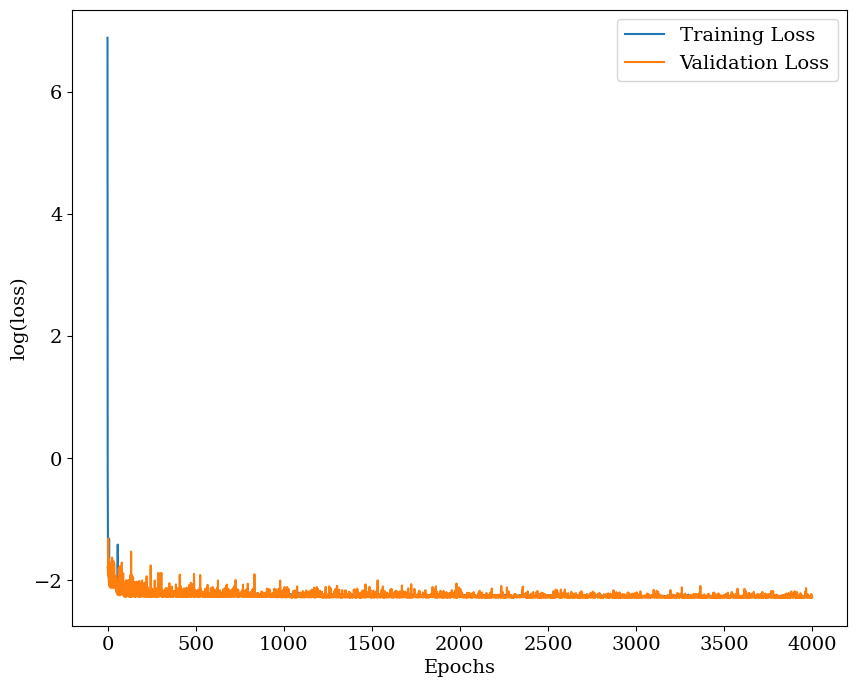
\includegraphics[width=.667\textwidth]{images/Chapter4/VGG19/vgg19_history.png}
\caption{As with VGG16, VGG19 is not able to learn in any way. Training and validation loss are close to each other throughout the whole training, indicating no overfitting but also no improvement in accuracy. } 
\label{fig:vgg19_best_history}
\end{figure}


Over all ten trainings, VGG19 was not able to give accurate predictions on neither the test nor the training set. As mentioned in \cref{vgg_16_res}, I do not know the core of this problem. It is possible though, that the model struggles to find any useful filters in training the convolutions, so that it is not able to detect any features. All it learned then was how to spread the galaxy clusters evenly to achieve the best possible loss without recognizing any galaxy cluster features. This would explain why the model only predicts values between $\log{(M_{500}^{\text{true}}/M_{\odot})} = 13.4$ and $\log{(M_{500}^{\text{true}}/M_{\odot})} = 14.4$, because the most clusters are within this mass range (see \autoref{fig:data_dist}).
All in all, VGG models seem to be difficult to train with galaxy cluster data and optimization would be needed to get useful results. A smaller learning rate could help to avoid the brought up issues.


\begin{figure}[H]
\centering
\begin{subfigure}{.46\textwidth}
  \centering
  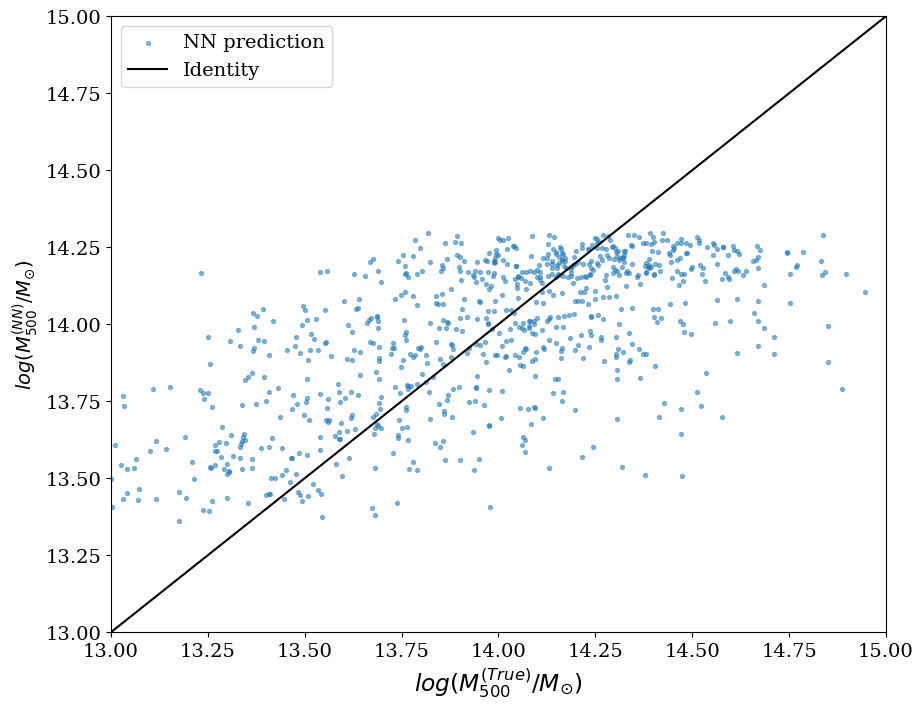
\includegraphics[width=\linewidth]{images/Chapter4/VGG19/vgg19_test.png}
  \caption{Model predictions on the test set.}
  \label{fig:best_perf_vgg19_a}
\end{subfigure}%
\hspace{.6em}
\begin{subfigure}{.46\textwidth}
  \centering
  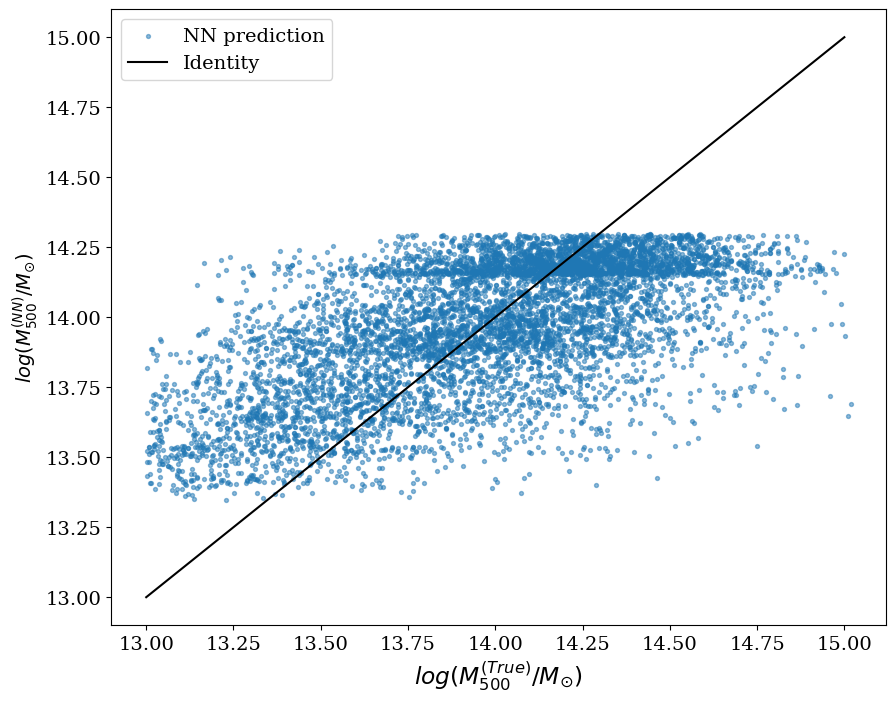
\includegraphics[width=\linewidth]{images/Chapter4/VGG19/vgg19_train.png}
  \caption{Model predictions on the training set.}
  \label{fig:best_perf_vgg19_b}
\end{subfigure}
\begin{subfigure}{.46\textwidth}
  \centering
  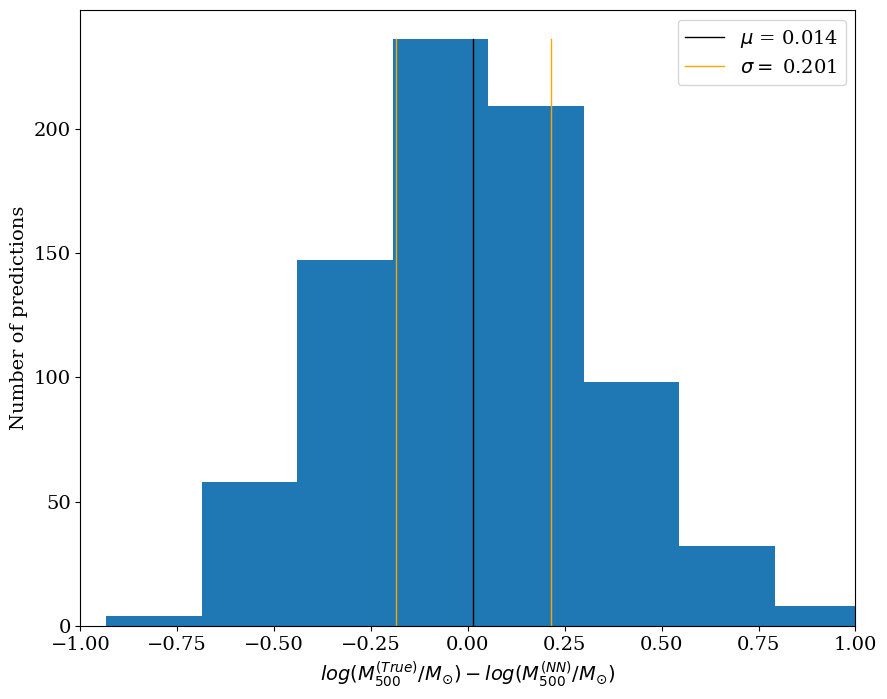
\includegraphics[width=\linewidth]{images/Chapter4/VGG19/vgg19_test_hist.png}
  \caption{Histogram of model predictions on the test set.}
  \label{fig:best_perf_vgg19_c}
\end{subfigure}%
\hspace{.6em}
\begin{subfigure}{.46\textwidth}
  \centering
  \includegraphics[width=\linewidth]{images/Chapter4/VGG19/vgg19_train_hist.png}
  \caption{Histogram of model predictions on the training set.}
  \label{fig:best_perf_vgg19_d}
\end{subfigure}
\caption{VGG19 is not able to predict accurately even on the training set. The results look similar to the predictions from VGG16} 
\label{fig:best_perf_vgg19}
\end{figure}



\subsection{ResNet}
ResNet is amongst the favorite deep neural networks in image recognition. Because of that, I chose three different models with increasing complexity and with an improved version, indicated by the \textit{V2} after the model's name. These are the training results.
\label{res_ResNet}

\subsubsection{ResNet50}
\subsubsection*{Training Insights}
ResNet training came with a lot of randomness over all different models. This is reflected in many trainings that could not perform well at all.
Some runs for example suffered from overfitting (see \autoref{fig:resnet50_bad_training}) while others weren't able to pick up any useful features and validation loss kept on spiking up every other epoch (see \autoref{fig:resnet50_best_history} between epoch 1000 and 1500).

\begin{figure}[H]
\centering
\includegraphics[width=.667\textwidth]{images/Chapter4/ResNet50/res50_bad_history.png}
\caption{ResNet50 with a bad training run. It occasionally reached lower validation loss values but in the end it started to overfit massively after a few thousand epochs of training, indicated by the increase of validation loss and simultaneous decrease of training loss.} 
\label{fig:resnet50_bad_training}
\end{figure}

Many trainings reached good estimations of a galaxy cluster masses relative to its other predictions but under-predicting all values. This is indicated by a smaller $\sigma$ with a high $\mu$ value.

\begin{figure}[H]
\centering
\begin{subfigure}{.46\textwidth}
\centering
\includegraphics[width=\textwidth]{images/Chapter4/ResNet50/best_but_not_pred.png}
\caption{Predictions from a ResNet50 model with good $\sigma$ but bad $\mu$. The model has difficulties with masses higher than $\log{(M_{500}^{\text{true}}/M_{\odot})} \sim 14$} 
\label{fig:bad_mu}
\end{subfigure}
\hspace{.6em}
\begin{subfigure}{.46\textwidth}
\centering
\includegraphics[width=\textwidth]{images/Chapter4/ResNet50/best_but_not.png}
\caption{Histogram of ResNet50 model predictions with good $\sigma$ but bad $\mu$. The whole histogram is shifted towards the right, caused by the positive $\mu$ value.} 
\label{fig:bad_mu_hist}
\end{subfigure}
\caption{A ResNet50 model that was able to get a good sense of the cluster mass in relation to other clusters but under-predicting almost all values, especially at masses higher than $\log{(M_{500}^{\text{true}}/M_{\odot})} \sim 14$.}
\label{fig:bad_mu_comp}
\end{figure}




\subsubsection*{Best Performing Model}
Because of the problems I mentioned before, I did not chose the model with the lowest $\sigma$ on the test set to be the best model because its average mass difference $\mu$ is quite big with $0.18$. Moreover, it had some massive over estimations on the training set. This makes the $\sigma$ and $\mu$ explode on this set. Because of that I went with a training that had a higher $\sigma$ on the test set with $\sigma = 0.185$ (rather than the $0.171$) but was more evenly spread around the identity with a $\mu$ of $0.035$.

\begin{figure}[H]
\centering
\includegraphics[width=.667\textwidth]{images/Chapter4/ResNet50/res50_best_history.png}
\caption{Best performing ResNet50 model after ten training runs. After more spikes in validation loss at the beginning, as the training loss kept on decreasing the validation loss settled at around $0.01$. A slightly lower validation loss after around $200$ epochs might be an indication for overfitting.} 
\label{fig:resnet50_best_history}
\end{figure}


\begin{figure}[H]
\centering
\begin{subfigure}{.46\textwidth}
  \centering
  \includegraphics[width=\linewidth]{images/Chapter4/ResNet50/res50_best_test.png}
  \caption{Model predictions on the test set.}
  \label{fig:best_perf_resnet50_a}
\end{subfigure}%
\hspace{.6em}
\begin{subfigure}{.46\textwidth}
  \centering
  \includegraphics[width=\linewidth]{images/Chapter4/ResNet50/res50_best_train.png}
  \caption{Model predictions on the training set.}
  \label{fig:best_perf_resnet50_b}
\end{subfigure}
\begin{subfigure}{.46\textwidth}
  \centering
  \includegraphics[width=\linewidth]{images/Chapter4/ResNet50/res50_best_test_hist.png}
  \caption{Histogram of model predictions on the test set.}
  \label{fig:best_perf_resnet50_c}
\end{subfigure}%
\hspace{.6em}
\begin{subfigure}{.46\textwidth}
  \centering
  \includegraphics[width=\linewidth]{images/Chapter4/ResNet50/res50_best_train_hist.png}
  \caption{Histogram of model predictions on the training set.}
  \label{fig:best_perf_resnet50_d}
\end{subfigure}
\caption{Prediction analysis for ResNet50 model. Predictions on the training set indicate overfitting.} 
\label{fig:best_perf_resnet50}
\end{figure}

On the test set the predictions are too high for smaller galaxy clusters, and too low for bigger galaxy clusters. All in all they are widely spread and are considerably worse than the basic CNN's best model.
The predictions on the training set look very similar to the predictions received in \autoref{fig:overf_comp_train}, indicating overfitting. This was also seen in the training history (see \autoref{fig:resnet50_best_history}), where the validation loss had its minimum after $200$ epochs. This shows that the model might be capable of accurate mass estimations after optimization. To improve the ResNet50 model, adjustments in training speed might yield better results.

\subsubsection{ResNet50V2}
\subsubsection*{Training Insights}
ResNet50V2 training was very similar to the other ResNets with some trainings yielding good results but also many trainings that were not able to pick up useful information from the images. Interestingly, nine out of the ten trainings ended up predicting masses lower than the actual masses, indicated by a positive $\mu$ value. Overall, ResNet50V2 was able to perform quite well on multiple training runs with a $\sigma < 0.15$ on three occasions.

\subsubsection*{Best Performing Model}
The best performing ResNet50V2 model was the second best performing deep learning model overall with a $\sigma < 0.14$. Despite the good sense for the relative masses, the model still predicted lower masses throughout the mass range resulting in a $\mu$ of $0.087$. The training itself did not seem to produce a good performing model at all with high validation losses until almost the end of training. Somehow, the model seemed to detect useful features just before the end of training, resulting in a good performance.

\begin{figure}[H]
\centering
\includegraphics[width=.667\textwidth]{images/Chapter4/Res50V2/resnet50V2_history.png}
\caption{Best performing ResNet50V2 model after ten training runs. Astonishingly, the training was quite poor until the training loss rapidly decreased from epoch 3600 on. The validation loss only settled to a low value just a few hundred epochs before the end of the training. } 
\label{fig:resnet50v2_best_history}
\end{figure}


\begin{figure}[H]
\centering
\begin{subfigure}{.46\textwidth}
  \centering
  \includegraphics[width=\linewidth]{images/Chapter4/Res50V2/resnet50v2_test.png}
  \caption{Model predictions on the test set.}
  \label{fig:best_perf_resnet50v2_a}
\end{subfigure}%
\hspace{.6em}
\begin{subfigure}{.46\textwidth}
  \centering
  \includegraphics[width=\linewidth]{images/Chapter4/Res50V2/resnet50v2_training.png}
  \caption{Model predictions on the training set.}
  \label{fig:best_perf_resnet50v2_b}
\end{subfigure}
\begin{subfigure}{.46\textwidth}
  \centering
  \includegraphics[width=\linewidth]{images/Chapter4/Res50V2/resnet50v2_test_hist.png}
  \caption{Histogram of model predictions on the test set.}
  \label{fig:best_perf_resnet50v2_c}
\end{subfigure}%
\hspace{.6em}
\begin{subfigure}{.46\textwidth}
  \centering
  \includegraphics[width=\linewidth]{images/Chapter4/Res50V2/resnet50v2_training_hist.png}
  \caption{Histogram of model predictions on the training set.}
  \label{fig:best_perf_resnet50v2_d}
\end{subfigure}
\caption{Prediction on the test and training set look similar. The standard deviation $\sigma$ on the training set is slightly lower which could be a sign for little overfitting.} 
\label{fig:best_perf_resnet50v2}
\end{figure}

The ResNet50V2 model seems to be quite good at galaxy cluster estimation. It comes close to the basic CNN ($\sigma \sim 0.13$) with a standard deviation of $\sigma \sim 0.14$. With some optimization in training speed, the number of epochs or the input image resolution, I can see this model outperforming the basic CNN in the future. 

\subsubsection{ResNet101}
\subsubsection*{Training Insights}
ResNet101 training was also similar to the other ResNet model's training. Many trainings did not produce good predictions and either suffered from too low mass estimations or other problems due to overfitting. 


\subsubsection*{Best Performing Model}

\begin{figure}[H]
\centering
\includegraphics[width=.667\textwidth]{images/Chapter4/Res101/res101_history.png}
\caption{Training history of the best performing ResNet101 model.} 
\label{fig:resnet101_best_history}
\end{figure}

The best ResNet101's training did not have as many spikes in validation loss as many of the other model's training had. The validation loss kept steady after about 1700 epochs of training. After just a few hundred epochs it was at a minimum after which it went up again. This is an indicator for overfitting because the training loss kept on decreasing afterwards. 

\begin{figure}[H]
\centering
\begin{subfigure}{.46\textwidth}
  \centering
  \includegraphics[width=\linewidth]{images/Chapter4/Res101/res101_test.png}
  \caption{Model predictions on the test set.}
  \label{fig:best_perf_resnet101_a}
\end{subfigure}%
\hspace{.6em}
\begin{subfigure}{.46\textwidth}
  \centering
  \includegraphics[width=\linewidth]{images/Chapter4/Res101/res101_train.png}
  \caption{Model predictions on the training set.}
  \label{fig:best_perf_resnet101_b}
\end{subfigure}
\begin{subfigure}{.46\textwidth}
  \centering
  \includegraphics[width=\linewidth]{images/Chapter4/Res101/res101_test_hist.png}
  \caption{Histogram of model predictions on the test set.}
  \label{fig:best_perf_resnet101_c}
\end{subfigure}%
\hspace{.6em}
\begin{subfigure}{.46\textwidth}
  \centering
  \includegraphics[width=\linewidth]{images/Chapter4/Res101/res101_train_hist.png}
  \caption{Histogram of model predictions on the training set.}
  \label{fig:best_perf_resnet101_d}
\end{subfigure}
\caption{Predictions on the training set are way better than the predictions on the test set which is a result of overfitting.} 
\label{fig:best_perf_resnet101}
\end{figure}

The overfitting can also be seen in \autoref{fig:best_perf_resnet101_a} and \autoref{fig:best_perf_resnet101_b} where the predictions on the test set are way worse than the predictions on the training set. On the other hand though, it was able to predict masses within the correct mass range, shown by the small $\mu$ compared to ResNet50V2 for instance. Overall, the performance of the ResNet101 model was not as good as other ResNet models such as ResNet50V2 and ResNet152V2 because the standard deviation of the difference between the predicted and the true mass was too high ($\sigma = 0.185$). The high variance in training also indicates that this model might not be ideal for galaxy cluster estimation, at least not without any optimization.


\subsubsection{ResNet101V2}
\subsubsection*{Training Insights}
Most ResNet101V2 trainings were not successful with only two trainings scoring a $\sigma < 0.18$. Apart from the models that massively over- or underestimated some galaxy masses, most models made smaller predictions resulting in a positive $\mu$. This behaviour was seen with most ResNet models. Especially for higher true masses, the difference between true and predicted mass was greater.


\subsubsection*{Best Performing Model}

\begin{figure}[H]
\centering
\includegraphics[width=.667\textwidth]{images/Chapter4/Res101V2/res101v2_history.png}
\caption{Training history of the best performing ResNet101V2 model.} 
\label{fig:resnet101v2_best_history}
\end{figure}

Despite the problems in training, the best performing ResNet101V2 model did quite well compared to the other models. With a $\sigma = 0.148$ it was the third best deep model of the ones I trained. Regardless of that, With a $\mu$ of $0.092$ it was the training that had the biggest difference between the predictions and the true masses of all trained models.


\begin{figure}[H]
\centering
\begin{subfigure}{.46\textwidth}
  \centering
  \includegraphics[width=\linewidth]{images/Chapter4/Res101V2/res101v2_test.png}
  \caption{Model predictions on the test set.}
  \label{fig:best_perf_resnet101v2_a}
\end{subfigure}%
\hspace{.6em}
\begin{subfigure}{.46\textwidth}
  \centering
  \includegraphics[width=\linewidth]{images/Chapter4/Res101V2/res101v2_training.png}
  \caption{Model predictions on the training set.}
  \label{fig:best_perf_resnet101v2_b}
\end{subfigure}
\begin{subfigure}{.46\textwidth}
  \centering
  \includegraphics[width=\linewidth]{images/Chapter4/Res101V2/res101v2_test_hist.png}
  \caption{Histogram of model predictions on the test set.}
  \label{fig:best_perf_resnet101v2_c}
\end{subfigure}%
\hspace{.6em}
\begin{subfigure}{.46\textwidth}
  \centering
  \includegraphics[width=\linewidth]{images/Chapter4/Res101V2/res101v2_training_hist.png}
  \caption{Histogram of model predictions on the training set.}
  \label{fig:best_perf_resnet101v2_d}
\end{subfigure}
\caption{Predictions on the training set had some very bad predictions, resulting in a very high $\sigma$ of $0.993$. Apart from that, the training set does not seem to be overfitted.} 
\label{fig:best_perf_resnet101v2}
\end{figure}

Interestingly, the model struggled with some of the training data by estimating a few values way too high or too low. This can be seen by the $\sigma$ of almost one. These estimations are not shown on \autoref{fig:best_perf_resnet101v2_b} and \autoref{fig:best_perf_resnet101v2_c} because they would make the important part of these plots unreadable. It is fascinating that in spite of these bad predictions, the model was still able to perform quite well.

\subsubsection{ResNet152}
\subsubsection*{Training Insights}
Not a single ResNet152 training managed to produce a model that is able to predict with a $\sigma < 2$. In combination with the long training times (see \autoref{tab:model_params}), this makes ResNet152 the least efficient ResNet model. Many models were not able to keep the predictions within the correct mass range and thus three trainings reached $\sigma$ values of over $10^4$.

\begin{figure}[H]
\centering
\begin{subfigure}{.46\textwidth}
\centering
\includegraphics[width=\textwidth]{images/Chapter4/Res152/res152_bad_1.png}
\caption{} 
\label{fig:res152_bad_a}
\end{subfigure}
\hspace{.6em}
\begin{subfigure}{.46\textwidth}
\centering
\includegraphics[width=\textwidth]{images/Chapter4/Res152/res152_bad_2.png}
\caption{} 
\label{fig:res152_bad_b}
\end{subfigure}
\caption{Two of the three very bad trainings of ResNet152. Validation loss kept on spiking up at many epochs. In \autoref{fig:res152_bad_b}, validation loss was steadily low for a few hundred epochs but spiked up again before the end of training.}
\label{fig:res152_bad}
\end{figure}


\subsubsection*{Best Performing Model}
The best ResNet152 model did not suffer from the spikes seen in \autoref{fig:res152_bad}. Nevertheless, predictions are not that accurate compared to the other models and considering the lower $\sigma$ at the training predictions, overfitting might be the cause of this.


\begin{figure}[H]
\centering
\includegraphics[width=.667\textwidth]{images/Chapter4/Res152/res152_history.png}
\caption{Training history of the best performing ResNet152 model.} 
\label{fig:resnet152_best_history}
\end{figure}

As seen in multiple other ResNet trainings, the model tends to estimate smaller galaxy clusters ($\log{(M_{500}^{\text{true}}/M_{\odot})} < 14$) too high and bigger galaxy clusters ($\log{(M_{500}^{\text{true}}/M_{\odot})} > 14$) too low. This feature can be seen in both the training and the test predictions. As a result of this, the overall $\mu$ value is close to zero.


\begin{figure}[H]
\centering
\begin{subfigure}{.46\textwidth}
  \centering
  \includegraphics[width=\linewidth]{images/Chapter4/Res152/res152_test.png}
  \caption{Model predictions on the test set.}
  \label{fig:best_perf_resnet152_a}
\end{subfigure}%
\hspace{.6em}
\begin{subfigure}{.46\textwidth}
  \centering
  \includegraphics[width=\linewidth]{images/Chapter4/Res152/res152_train.png}
  \caption{Model predictions on the training set.}
  \label{fig:best_perf_resnet152_b}
\end{subfigure}
\begin{subfigure}{.46\textwidth}
  \centering
  \includegraphics[width=\linewidth]{images/Chapter4/Res152/res152_test_hist.png}
  \caption{Histogram of model predictions on the test set.}
  \label{fig:best_perf_resnet152_c}
\end{subfigure}%
\hspace{.6em}
\begin{subfigure}{.46\textwidth}
  \centering
  \includegraphics[width=\linewidth]{images/Chapter4/Res152/res152_train_hist.png}
  \caption{Histogram of model predictions on the training set.}
  \label{fig:best_perf_resnet152_d}
\end{subfigure}
\caption{ResNet152 training results are worse than all the other ResNet models trained. The better training predictions could be explained by overfitting.} 
\label{fig:best_perf_resnet152}
\end{figure}

\subsubsection{ResNet152V2}
\subsubsection*{Training Insights}
ResNet152V2 was amongst the most successful of all models trained. It achieved a standard deviation of $ \sigma \le 1.8$ on five occasions. As seen in the best performing model (see \autoref{fig:resnet152v2_best_history}), many trainings began with only modest progress but after a few thousand epochs the training was able to make huge improvements and training loss decreased rapidly. This also allowed the validation loss to settle after repeated outbursts. The ability to find useful features after long training and to be able to continue training without overfitting is one of the key advantages I witnessed during training.   
\subsubsection*{Best Performing Model}
ResNet152V2 was able to make the best predictions out of all nine trained models. With a $\sigma$ of $1.34$ it was only marginally worse than the basic CNN with a standard deviation of $\sigma \sim 1.30$. As brought up before, ResNet152V2 training was able to make rapid improvements after around 1800 epochs and both training and validation loss was able to improve because of that. Moreover, there is no visible overfitting going on which is indicated by the steady validation loss and the training predictions (see \autoref{fig:best_perf_resnet152v2_b}).

\begin{figure}[H]
\centering
\includegraphics[width=.667\textwidth]{images/Chapter4/Res152V2/res152v2_history.png}
\caption{Training history of the best performing ResNet152V2 model.} 
\label{fig:resnet152v2_best_history}
\end{figure}

As seen with other ResNet models, this model also overestimated smaller galaxy clusters and underestimates the masses of bigger galaxy clusters with an overall trend on underestimating ($\mu = 0.055$). Especially in a mass range between $\log{(M_{500}^{\text{true}}/M_{\odot})} = 14$ and $\log{(M_{500}^{\text{true}}/M_{\odot})} = 14.5$ the predictions seem to be even better which could mean that it is easier for the model to estimate the masses of larger galaxy clusters.

\begin{figure}[H]
\centering
\begin{subfigure}{.46\textwidth}
  \centering
  \includegraphics[width=\linewidth]{images/Chapter4/Res152V2/res152v2_test.png}
  \caption{Model predictions on the test set.}
  \label{fig:best_perf_resnet152v2_a}
\end{subfigure}%
\hspace{.6em}
\begin{subfigure}{.46\textwidth}
  \centering
  \includegraphics[width=\linewidth]{images/Chapter4/Res152V2/res152v2_train.png}
  \caption{Model predictions on the training set.}
  \label{fig:best_perf_resnet152v2_b}
\end{subfigure}
\begin{subfigure}{.46\textwidth}
  \centering
  \includegraphics[width=\linewidth]{images/Chapter4/Res152V2/res152v2_test_hist.png}
  \caption{Histogram of model predictions on the test set.}
  \label{fig:best_perf_resnet152v2_c}
\end{subfigure}%
\hspace{.6em}
\begin{subfigure}{.46\textwidth}
  \centering
  \includegraphics[width=\linewidth]{images/Chapter4/Res152V2/res152v2_train_hist.png}
  \caption{Histogram of model predictions on the training set.}
  \label{fig:best_perf_resnet152v2_d}
\end{subfigure}
\caption{Results of the best overall performing deep network. $\sigma$ is quite high at the training set as a result of a few very bad predictions outside of the mass range. } 
\label{fig:best_perf_resnet152v2}
\end{figure}

One thing worth noting with the training predictions is that the model put a few galaxy clusters on masses that are outside of the mass range. This results in the standard deviation of the training set being way higher ($\sigma = 0.319$) than the standard deviation of the test set. This makes it a bit harder to spot overfitting but considering the prediction's spread in \autoref{fig:best_perf_resnet152v2_b} the model is most likely not overfitting. Finding improvements to this model might not be so easy but as with the other deep models a smaller learning rate could help to improve prediction accuracy.

\subsection{EfficientNet}
The final architecture that I want to test is also the most recently developed model. It uses machine learning to optimize the model's architecture to reach higher accuracies with lower parameters.

\subsubsection{EfficientNet-B7}
\subsubsection*{Training Insights}
EfficientNet did not produce useful predictions on any of the ten training runs. Even the best model struggled to estimate galaxy cluster masses precisely. Especially with lower mass clusters, the model was not able to get close to the true values as seen in \autoref{fig:best_perf_EffB7_a} and \ref{fig:best_perf_EffB7_b}. The predictions look somewhat similar to the VGG predictions, in that they are cut off at a certain value, in this case at around $\log{(M_{500}^{\text{true}}/M_{\odot})} \sim 13.5$.

\subsubsection*{Best Performing Model}
The best performing EfficientNetB7 model suffered from the same problems as the other EfficientNetB7 models trained. Its predictions are cut of at the lower end and on the training predictions, two lines are visible where the model seemed to prefer two mass areas for its predictions.

\begin{figure}[H]
\centering
\includegraphics[width=.667\textwidth]{images/Chapter4/EffB7/eff_history.png}
\caption{Training history of the best performing EfficientNetB7 model. The spiking validation loss indicates that the training did not produce good results.} 
\label{fig:EffB7_best_history}
\end{figure}
While the training loss kept decreasing, the validation loss was spiking at many epochs during training. The model seemed to have problems finding anything useful to improve validation accuracy. As seen in the model's predictions, the model was not even able to make predictions in the correct mass range.


\begin{figure}[H]
\centering
\begin{subfigure}{.46\textwidth}
  \centering
  \includegraphics[width=\linewidth]{images/Chapter4/EffB7/eff_test.png}
  \caption{Model predictions on the test set.}
  \label{fig:best_perf_EffB7_a}
\end{subfigure}%
\hspace{.6em}
\begin{subfigure}{.46\textwidth}
  \centering
  \includegraphics[width=\linewidth]{images/Chapter4/EffB7/eff_train.png}
  \caption{Model predictions on the training set.}
  \label{fig:best_perf_EffB7_b}
\end{subfigure}
\begin{subfigure}{.46\textwidth}
  \centering
  \includegraphics[width=\linewidth]{images/Chapter4/EffB7/eff_test_hist.png}
  \caption{Histogram of model predictions on the test set.}
  \label{fig:best_perf_EffB7_c}
\end{subfigure}%
\hspace{.6em}
\begin{subfigure}{.46\textwidth}
  \centering
  \includegraphics[width=\linewidth]{images/Chapter4/EffB7/eff_train_hist.png}
  \caption{Histogram of model predictions on the training set.}
  \label{fig:best_perf_EffB7_d}
\end{subfigure}
\caption{Results of the best EfficientNetB7 model.} 
\label{fig:best_perf_EffB7}
\end{figure}

Because of these problems, the overall prediction accuracy is not close to the best ResNets or the basic CNN with a $\sigma$ of $0.183$ on the test set. Astonishingly, despite the low training loss, the predictions on the training set are not overfitted or anywhere near the identity (see \autoref{fig:best_perf_EffB7_b}). Considering the enormous training time for this model and its lacking accuracy, I would not recommend further investigation of this model for galaxy cluster mass estimation.

\newpage
\subsection{Full Results}
\label{Results}
To evaluate how the different models were able to perform, I prepared the resulting data in a few different ways. First, I will compare the training histories for the training and validation loss in \autoref{fig:history_all}. Afterwards I will inspect the most accurate of all deep models ResNet152V2 and compare it with the basic CNN and its predictions. At the end, in \autoref{tab:results_table} I set side by side all key metrics of the best performing models.

\subsubsection{Training History Comparison}

Training resulted in many different outcomes depending on the model. To help compare the training history of all models consider \autoref{fig:history_all}. The training history of both the training and validation loss is shown in one plot each for easy comparison. Because of the many spikes seen in training, the losses are smoothed using the simple moving average (SME) \eqref{rol_mean} with $k = 100$ entries taken into account for smoothing a single value.

\begin{figure}[H]
\begin{subfigure}{.5\textwidth}
    \centering
    \includegraphics[width=\linewidth]{images/Chapter4/Results/tr_loss_hist.png}
    \caption{Training loss for all models}
    \label{fig:history_all_training_loss}
\end{subfigure}
\begin{subfigure}{.5\textwidth}
    \centering
    \includegraphics[width=\linewidth]{images/Chapter4/Results/val_loss_hist.png}
    \caption{Validation loss for all models}
    \label{fig:history_all_validation_loss}
\end{subfigure}
\caption{Training loss history for all deep models gives a good comparison of different learning outcomes. The VGG models were not able to predict accurately and thus their training loss could not improve over the 4000 epochs. The other models either improved very quickly at the beginning or were able to find helpful features later in training. For the validation loss (\textit{right}) only the best seven models are shown for easier comparison. Remember that the basic CNN shown in this graphic is not the best performing model because it only trained for around 100 epochs. Instead the overfitted model from \autoref{fig:basic_cnn_overf} is shown to compare it to the deep models. The training and validation loss histories are smoothed using the simple moving average (SMA) \eqref{rol_mean} with $k = 100$ entries taken for smoothing.}
\label{fig:history_all}
\end{figure}

Especially the two best performing deep models ResNet50V2 and ResNet152V2 are clearly separated from the other models in validation loss (see \autoref{fig:history_all_validation_loss}) with values around $-2.9$. One thing I don't yet understand is that the training loss of the overfitted baseline network is considerably higher ($\sim -7$) than the training loss of the other deep models ($< -8 $) considering the way more accurate predictions on the training set for the baseline model. I do not know where this discrepancy comes from but it would be very interesting to investigate this further. 

\subsubsection{Best Performing Deep CNN vs. Basic CNN}
ResNet152V2 was able to get closest to the basic CNN in terms of validation loss and standard deviation on the test set with $\sigma = 0.134$. The biggest difference between these two models is in the expected value $\mu$, where the basic CNN was able to perform really well with $\mu \sim 0$. ResNet152V2 struggled a little bit with predicting smaller values than the true masses which resulted in a $\mu$ value of $0.055$. Obviously, the deep model is no way near as efficient as the basic CNN with a training time of roughly one day for each run of 4000 epochs while the basic CNN only takes minutes to get more accurate predictions. 

\begin{figure}[H]
\begin{subfigure}{.5\textwidth}
    \centering
    \includegraphics[width=\linewidth]{images/Chapter4/Results/test_ResNet152V2_scatter.png}
    \label{fig:test_ResNet152V2_scatter}
\end{subfigure}
\begin{subfigure}{.5\textwidth}
    \centering
    \includegraphics[width=\linewidth]{images/Chapter4/Results/test_ResNet152V2_hist.png}
    \label{fig:test_ResNet152V2_hist}
\end{subfigure}
\label{fig:res52v2_all}
\caption{ResNet152V2 was able to predict almost as accurately as the basic CNN. The deep model's predictions are slightly smaller than the true masses resulting in a positive $\mu$. The basic CNN was able to perform a little bit better in this regard with a $\mu$ of almost zero.}
\end{figure}

\begin{figure}[H]
\begin{subfigure}{.5\textwidth}
    \centering
    \includegraphics[width=\linewidth]{images/Chapter4/Results/training_ResNet152V2_scatter.png}
    \label{fig:training_ResNet152V2_scatter}
\end{subfigure}
\begin{subfigure}{.5\textwidth}
    \centering
    \includegraphics[width=\linewidth]{images/Chapter4/Results/training_ResNet152V2_hist.png}
    \label{fig:training_ResNet152V2_hist}
\end{subfigure}
\label{fig:res52v2_all_training}
\caption{Predictions on the training set look similar too. ResNet152V2 again predicted slightly lower masses than the baseline CNN. The standard deviation $\sigma$ is way bigger for the deep model because of a few very bad fits outside the mass range.}
\end{figure}

All comparison plots between the deep models and the baseline can be found in \cref{app}.\\

Another aspect worth mentioning is the training randomness especially with deep models. I had very different results for ResNet152V2 (and all ResNet models) for every single training run where only one was able to get this close to the basic CNN. The baseline however was able to make accurate predictions in almost every training run with way less randomness and exploding validation losses. This could be caused by the deep model's complexity with over 200 times more trainable parameters (see \autoref{tab:model_params}). This problem could be solved with a careful selection of the learning rate. Even features like a variable learning rate, where the learning rate is changed depending on the model's training, could improve training efficiency for the deep models. This is only one of many ways though to help increase the effectiveness of these long training runs. I will discuss how one could continue with optimization of deep models for galaxy cluster estimation in the conclusion in \cref{conclusion}.

\subsubsection{Table}
For the results of all best performing models consider \autoref{tab:results_table}.
\begin{table*}[h]
\centering
\begin{tabular}{@{}ccccccc@{}}\toprule
Model Name & Training Loss* & Validation Loss* & $\sigma^{\text{test}}$ & $\mu^{\text{test}}$ & $\sigma^{\text{train}}$ & $\mu^{\text{train}}$ \\
\midrule
Basic CNN & $0.046^{\dag}$ & $0.047^{\dag}$ & $0.13$ & $0$ & $0.122$ & $0.003$\\
VGG16 & $0.104$ & $0.102$ & $0.2$ & $-0.019$ & $0.196$ & $-0.027$\\
VGG19 & $0.103$ & $0.102$ & $0.201$ & $0.014$ & $0.195$ & $0.006$ \\
ResNet50 & $0.001$ & $0.09$ & $0.185$ & $-0.035$ & $0.147$& $0.04$\\
ResNet50V2 & $0.0001$ & $0.056$ & $0.14$ & $0.087$ & $0.127$ & $0.087$\\
ResNet101 & $0.0001$ & $0.093$ & $0.182$ & $0.056$ & $0.142$ & $0.055$\\
ResNet101V2 & $0.0001$  &  $0.064$ & $0.148$ & $0.092$ & $0.993$ & $0.092$\\
ResNet152 & $0.0002$ & $0.114$ & $0.201$ & $0.001$ & $0.150$ & $0.017$\\
ResNet152V2 & $0.0001$  & $0.052$ & $0.134$ & $0.055$ & $0.319$ & $0.056$  \\
EfficientNet-B7 &  $0.0002$ & $0.101$ & $0.183$ & $0.037$ & $0.190$ & $0.045$ \\
\bottomrule
\end{tabular}
\caption{Complete training results for the best performing models. It shows how the improved ResNet versions were able to perform better than their predecessors. The VGG and EfficientNet models did not produce accurate results.  *After the last epoch, $^{\dag}$training and validation loss for the epoch with the lowest validation loss value, 15 epochs before the training ended.}
\label{tab:results_table}
\end{table*}









\newpage
\section{Conclusion}
\label{conclusion}
From the three different architectures tested in my thesis, ResNet came out as clear winner, being able to make predictions almost as accurate as the baseline network. This is a great starting point for future attempts to optimize the deep models further and clearly shows that it is possible to use more complex neural networks for X-ray astronomy. The pipeline I built for training and testing a deep neural network was made in such a way that it is easy to rerun the training with different parameters such as different learning rates, custom weights, validation loss monitoring to spot overfitting earlier during training and many more. This allows to further investigate which parameters can help to improve accuracy to beat the baseline CNN. It is even possible to try different neural network models apart from VGG, ResNet and EfficientNet to see if there might be other architectures that work for galaxy cluster mass estimation. For future attempts at improving these deep models, I would suggest to start with ResNet50V2 instead of the more accurate ResNet152V2 because it was almost as accurate as the complex model but with way less training time. Because of the similarities of the two models, I expect the same optimizations to work on both models which makes it unnecessarily more complicated to try to find them for the bigger model first. It would be very interesting to see if a neural network powered hyperparameter tuning would help to find better results in the future. \\
One thing that I find especially interesting is if there is a big difference in accuracy with no pretraining of the deep neural networks. I can imagine that the pretraining might limit the possible outcomes of the training and thus training without it could improve accuracy. Unfortunately, the time frame for a Bachelor's Thesis was not enough to test all of this.\\
Another very interesting investigation would be to see whether the model excels at certain galaxy cluster features such as big or small masses or specific redshifts. One could also use a way bigger dataset for training because it is possible to simulate any number of galaxy clusters and see the outcomes of this. Also changing the resolution of the input images or the frequency bands used could have interesting outcomes. \\ 

Astronomy in particular is driven by enormous amounts of data that is simply not possible to be scanned through by humans and machine learning is able to not only detect features on a human level of accuracy, but way better. Because most of astronomy's data is in the form of images, CNNs will play a key role in future discoveries because they proved to be exceptionally good at extracting features. With the rate of improvement seen over the last years, even better models and faster GPUs will accelerate the trend of using CNNs in astronomy and science in general.  \\

After over 40 days of total training time I have gained a lot of insight into the training of neural networks and especially the problems that come with it. Although not reflected in this paper, most of this thesis work was put into figuring out how to solve never ending programming problems in order to get the models to train. But once the training pipeline was built, it was possible to train multiple models at a time. I hope this pipeline will help future development and optimization of deep neural networks in order to improve galaxy mass estimation. 
\newpage

% ------------------------------------------------------------------------------
% APPENDIX ---------------------------------------------------------------------
% ------------------------------------------------------------------------------
    
\pagenumbering{Roman}

\setcounter{page}{1} % CHANGE

\appendix

\section{Appendix}
\label{app}
\subsection{Additional Equations}

Simple moving mean:

\begin{equation}
    \text{SMA}_k = \frac{p_{n-k+1}+p_{n-k+2}+\cdots+p_n}{k} = \frac{1}{k}\sum_{i=n-k+1}^np_i,
    \label{rol_mean}
\end{equation}

where $p_i$ is a data point, $n$ the number of total data points and $k$ the number of entries taken into account.

\subsection{Additional Plots}
Some plots did not fit into the main thesis either because of their format or their content but I think they are still worth showing. The first shows a comparison between ImageNet images with their label and the galaxy cluster images I used for training with their label. It is supposed to show the similarity in task between classification for the ILSVRC and classification of galaxy cluster masses.

\begin{figure}[H]
 \centering
 \includegraphics[width=0.8\textwidth]{images/Chapter2/imagenet_clusters.png}
 \caption{(\textit{Left}) images from ImageNet catalogue with labels (credit: ImageNet). (\textit{Right}) galaxy clusters from eFEDS simulation with mass and redshift as labels.}
 \label{fig:imagenet_clusters}
\end{figure}

The next plot shows the architectures of VGG19 and the shallower ResNet34 residual neural network.


\begin{figure}[H]
\centering
\includegraphics[width=.55\textwidth]{images/Chapter2/4-Figure3-1.png}
\caption{Comparison between VGG16's and ResNet's architecture.} 
\label{fig:Res34}
\end{figure} 

Finally, here are all the comparing results of the best deep models with the baseline model on the test and training set.


\begin{figure}[H]
\centering
\begin{subfigure}{.325\textwidth}
    \centering
    \includegraphics[width=\linewidth]{images/Chapter4/Results/test_VGG16_scatter.png}
    \label{fig:test_VGG16_scatter}
    \caption{VGG16}
\end{subfigure}
\begin{subfigure}{.325\textwidth}
    \centering
    \includegraphics[width=\linewidth]{images/Chapter4/Results/test_VGG19_scatter.png}
    \label{fig:test_VGG19_scatter}
    \caption{VGG19}
\end{subfigure}
\begin{subfigure}{.325\textwidth}
    \centering
    \includegraphics[width=\linewidth]{images/Chapter4/Results/test_ResNet50_scatter.png}
    \label{fig:test_ResNet50_scatter}
    \caption{ResNet50}
\end{subfigure}
\begin{subfigure}{.325\textwidth}
    \centering
    \includegraphics[width=\linewidth]{images/Chapter4/Results/test_ResNet50V2_scatter.png}
    \label{fig:test_ResNet50V2_scatter}
    \caption{ResNet50V2}
\end{subfigure}
\begin{subfigure}{.325\textwidth}
    \centering
    \includegraphics[width=\linewidth]{images/Chapter4/Results/test_ResNet101_scatter.png}
    \label{fig:test_ResNet101_scatter}
    \caption{ResNet101}
\end{subfigure}
\begin{subfigure}{.325\textwidth}
    \centering
    \includegraphics[width=\linewidth]{images/Chapter4/Results/test_ResNet101V2_scatter.png}
    \label{fig:test_ResNet101V2_scatter}
    \caption{ResNet101V2}
\end{subfigure}
\begin{subfigure}{.325\textwidth}
    \centering
    \includegraphics[width=\linewidth]{images/Chapter4/Results/test_ResNet152_scatter.png}
    \label{fig:test_ResNet152_scatter}
    \caption{ResNet152}
\end{subfigure}
\begin{subfigure}{.325\textwidth}
    \centering
    \includegraphics[width=\linewidth]{images/Chapter4/Results/test_ResNet152V2_scatter.png}
    \label{fig:test_ResNet152V2_scatter}
    \caption{ResNet152V2}
\end{subfigure}
\begin{subfigure}{.325\textwidth}
    \centering
    \includegraphics[width=\linewidth]{images/Chapter4/Results/test_EfficientNetB7_scatter.png}
    \label{fig:test_EfficientNetB7_scatter}
    \caption{EfficientNetB7}
\end{subfigure}
\caption{Comparison between each deep model's best predictions (\textit{blue}) and the best predictions from the basic CNN (\textit{grey}) in the test set.}
\end{figure}

\begin{figure}[H]
\centering
\begin{subfigure}{.325\textwidth}
    \centering
    \includegraphics[width=\linewidth]{images/Chapter4/Results/test_VGG16_hist.png}
    \label{fig:test_VGG16_hist}
    \caption{VGG16}
\end{subfigure}
\begin{subfigure}{.325\textwidth}
    \centering
    \includegraphics[width=\linewidth]{images/Chapter4/Results/test_VGG19_hist.png}
    \label{fig:test_VGG19_hist}
    \caption{VGG19}
\end{subfigure}
\begin{subfigure}{.325\textwidth}
    \centering
    \includegraphics[width=\linewidth]{images/Chapter4/Results/test_ResNet50_hist.png}
    \label{fig:test_ResNet50_hist}
    \caption{ResNet50}
\end{subfigure}
\begin{subfigure}{.325\textwidth}
    \centering
    \includegraphics[width=\linewidth]{images/Chapter4/Results/test_ResNet50V2_hist.png}
    \label{fig:test_ResNet50V2_hist}
    \caption{ResNet50V2}
\end{subfigure}
\begin{subfigure}{.325\textwidth}
    \centering
    \includegraphics[width=\linewidth]{images/Chapter4/Results/test_ResNet101_hist.png}
    \label{fig:test_ResNet101_hist}
    \caption{ResNet101}
\end{subfigure}
\begin{subfigure}{.325\textwidth}
    \centering
    \includegraphics[width=\linewidth]{images/Chapter4/Results/test_ResNet101V2_hist.png}
    \label{fig:test_ResNet101V2_hist}
    \caption{ResNet101V2}
\end{subfigure}
\begin{subfigure}{.325\textwidth}
    \centering
    \includegraphics[width=\linewidth]{images/Chapter4/Results/test_ResNet152_hist.png}
    \label{fig:test_ResNet152_hist}
    \caption{ResNet152}
\end{subfigure}
\begin{subfigure}{.325\textwidth}
    \centering
    \includegraphics[width=\linewidth]{images/Chapter4/Results/test_ResNet152V2_hist.png}
    \label{fig:test_ResNet152V2_hist}
    \caption{ResNet152V2}
\end{subfigure}
\begin{subfigure}{.325\textwidth}
    \centering
    \includegraphics[width=\linewidth]{images/Chapter4/Results/test_EfficientNetB7_hist.png}
    \label{fig:test_EfficientNetB7_hist}
    \caption{EfficientNetB7}
\end{subfigure}
\caption{Comparison histograms between each deep model's best predictions (\textit{blue}) and the best predictions from the basic CNN (\textit{grey}) on the test set.}
\end{figure}





\begin{figure}[H]
\centering
\begin{subfigure}{.325\textwidth}
    \centering
    \includegraphics[width=\linewidth]{images/Chapter4/Results/training_VGG16_scatter.png}
    \label{fig:training_VGG16_scatter}
    \caption{VGG16}
\end{subfigure}
\begin{subfigure}{.325\textwidth}
    \centering
    \includegraphics[width=\linewidth]{images/Chapter4/Results/training_VGG19_scatter.png}
    \label{fig:training_VGG19_scatter}
    \caption{VGG19}
\end{subfigure}
\begin{subfigure}{.325\textwidth}
    \centering
    \includegraphics[width=\linewidth]{images/Chapter4/Results/training_ResNet50_scatter.png}
    \label{fig:training_ResNet50_scatter}
    \caption{ResNet50}
\end{subfigure}
\begin{subfigure}{.325\textwidth}
    \centering
    \includegraphics[width=\linewidth]{images/Chapter4/Results/training_ResNet50V2_scatter.png}
    \label{fig:training_ResNet50V2_scatter}
    \caption{ResNet50V2}
\end{subfigure}
\begin{subfigure}{.325\textwidth}
    \centering
    \includegraphics[width=\linewidth]{images/Chapter4/Results/training_ResNet101_scatter.png}
    \label{fig:training_ResNet101_scatter}
    \caption{ResNet101}
\end{subfigure}
\begin{subfigure}{.325\textwidth}
    \centering
    \includegraphics[width=\linewidth]{images/Chapter4/Results/training_ResNet101V2_scatter.png}
    \label{fig:training_ResNet101V2_scatter}
    \caption{ResNet101V2}
\end{subfigure}
\begin{subfigure}{.325\textwidth}
    \centering
    \includegraphics[width=\linewidth]{images/Chapter4/Results/training_ResNet152_scatter.png}
    \label{fig:training_ResNet152_scatter}
    \caption{ResNet152}
\end{subfigure}
\begin{subfigure}{.325\textwidth}
    \centering
    \includegraphics[width=\linewidth]{images/Chapter4/Results/training_ResNet152V2_scatter.png}
    \label{fig:training_ResNet152V2_scatter}
    \caption{ResNet152V2}
\end{subfigure}
\begin{subfigure}{.325\textwidth}
    \centering
    \includegraphics[width=\linewidth]{images/Chapter4/Results/training_EfficientNetB7_scatter.png}
    \label{fig:training_EfficientNetB7_scatter}
    \caption{EfficientNetB7}
\end{subfigure}
\caption{Comparison between each deep model's best predictions (\textit{blue}) and the best predictions from the basic CNN (\textit{grey}) on the training set.}
\end{figure}

\begin{figure}[H]
\centering
\begin{subfigure}{.325\textwidth}
    \centering
    \includegraphics[width=\linewidth]{images/Chapter4/Results/training_VGG16_hist.png}
    \label{fig:training_VGG16_hist}
    \caption{VGG16}
\end{subfigure}
\begin{subfigure}{.325\textwidth}
    \centering
    \includegraphics[width=\linewidth]{images/Chapter4/Results/training_VGG19_hist.png}
    \label{fig:training_VGG19_hist}
    \caption{VGG19}
\end{subfigure}
\begin{subfigure}{.325\textwidth}
    \centering
    \includegraphics[width=\linewidth]{images/Chapter4/Results/training_ResNet50_hist.png}
    \label{fig:training_ResNet50_hist}
    \caption{ResNet50}
\end{subfigure}
\begin{subfigure}{.325\textwidth}
    \centering
    \includegraphics[width=\linewidth]{images/Chapter4/Results/training_ResNet50V2_hist.png}
    \label{fig:training_ResNet50V2_hist}
    \caption{ResNet50V2}
\end{subfigure}
\begin{subfigure}{.325\textwidth}
    \centering
    \includegraphics[width=\linewidth]{images/Chapter4/Results/training_ResNet101_hist.png}
    \label{fig:training_ResNet101_hist}
    \caption{ResNet101}
\end{subfigure}
\begin{subfigure}{.325\textwidth}
    \centering
    \includegraphics[width=\linewidth]{images/Chapter4/Results/training_ResNet101V2_hist.png}
    \label{fig:training_ResNet101V2_hist}
    \caption{ResNet101V2}
\end{subfigure}
\begin{subfigure}{.325\textwidth}
    \centering
    \includegraphics[width=\linewidth]{images/Chapter4/Results/training_ResNet152_hist.png}
    \label{fig:training_ResNet152_hist}
    \caption{ResNet152}
\end{subfigure}
\begin{subfigure}{.325\textwidth}
    \centering
    \includegraphics[width=\linewidth]{images/Chapter4/Results/training_ResNet152V2_hist.png}
    \label{fig:training_ResNet152V2_hist}
    \caption{ResNet152V2}
\end{subfigure}
\begin{subfigure}{.325\textwidth}
    \centering
    \includegraphics[width=\linewidth]{images/Chapter4/Results/training_EfficientNetB7_hist.png}
    \label{fig:training_EfficientNetB7_hist}
    \caption{EfficientNetB7}
\end{subfigure}
\caption{Comparison histograms between each deep model's best predictions (\textit{blue}) and the best predictions from the basic CNN (\textit{grey}) on the training set.}
\end{figure}
\newpage

\section{Electronic appendix}
\label{el_app}

All of the code used and developed during this work is available on my gitlab project at:

\url{https://gitlab.physik.uni-muenchen.de/krippendorf-lab/bachelor-ml-cluster-masses}\\

Please note that the code is not publicly available because it is subject to ongoing scientific research. Please contact Dr. Sven Krippendorf for access to my code and the data used to train the neural networks.

\newpage
    
% ------------------------------------------------------------------------------
% BIBLIOGRAPHY -----------------------------------------------------------------
% ------------------------------------------------------------------------------
\nocite{*}
\RaggedRight
\bibliography{bibliography}
\bibliographystyle{dcu}
\newpage

% ------------------------------------------------------------------------------
% DECLARATION OF AUTHORSHIP-----------------------------------------------------
% ------------------------------------------------------------------------------

\Large
\noindent
\textbf{Declaration of authorship} 
\vspace{0.5cm}
\noindent
\normalsize

I hereby declare that the report submitted is my own unaided work. All direct 
or indirect sources used are acknowledged as references. I am aware that the 
Thesis in digital form can be examined for the use of unauthorized aid and in 
order to determine whether the report as a whole or parts incorporated in it may 
be deemed as plagiarism. For the comparison of my work with existing sources I 
agree that it shall be entered in a database where it shall also remain after 
examination, to enable comparison with future Theses submitted. Further rights 
of reproduction and usage, however, are not granted here. This paper was not 
previously presented to another examination board and has not been published.
\\

\vspace{1cm}
\textcolor{orange}{Munich, 13\textsuperscript{th} of September, 2023} \\

\vspace{3cm}

\noindent\rule{0.5\textwidth}{0.4pt} \\

\textcolor{orange}{Matthias Heim}

% ------------------------------------------------------------------------------

\end{document}
